\section{Spectrum Estimation}

\subsection{Discrete Fourier Transform Basics}\label{sec:dft_basics}

\noindent{}a. The ideal Fourier (magnitude) spectrum of a 20 Hz sine wave and the theoretical continuous frequency DTFT (magnitude) spectrum for a windowed sine wave at 20 Hz are shown below. Since a sine wave is a real periodic signal, we expect the ideal magnitude spectrum to be an even discrete function consisting of only dirac delta functions. The magnitude spectrum of the rectangular window used is a \textit{sinc} function. The ideal magnitude spectrum is convoluted with the \textit{sinc} function to produce the theoretical continuous magnitude spectrum; it is clear that the window has caused smearing and leaked the ideal spectrum.

\begin{figure}[H]
\centering{}
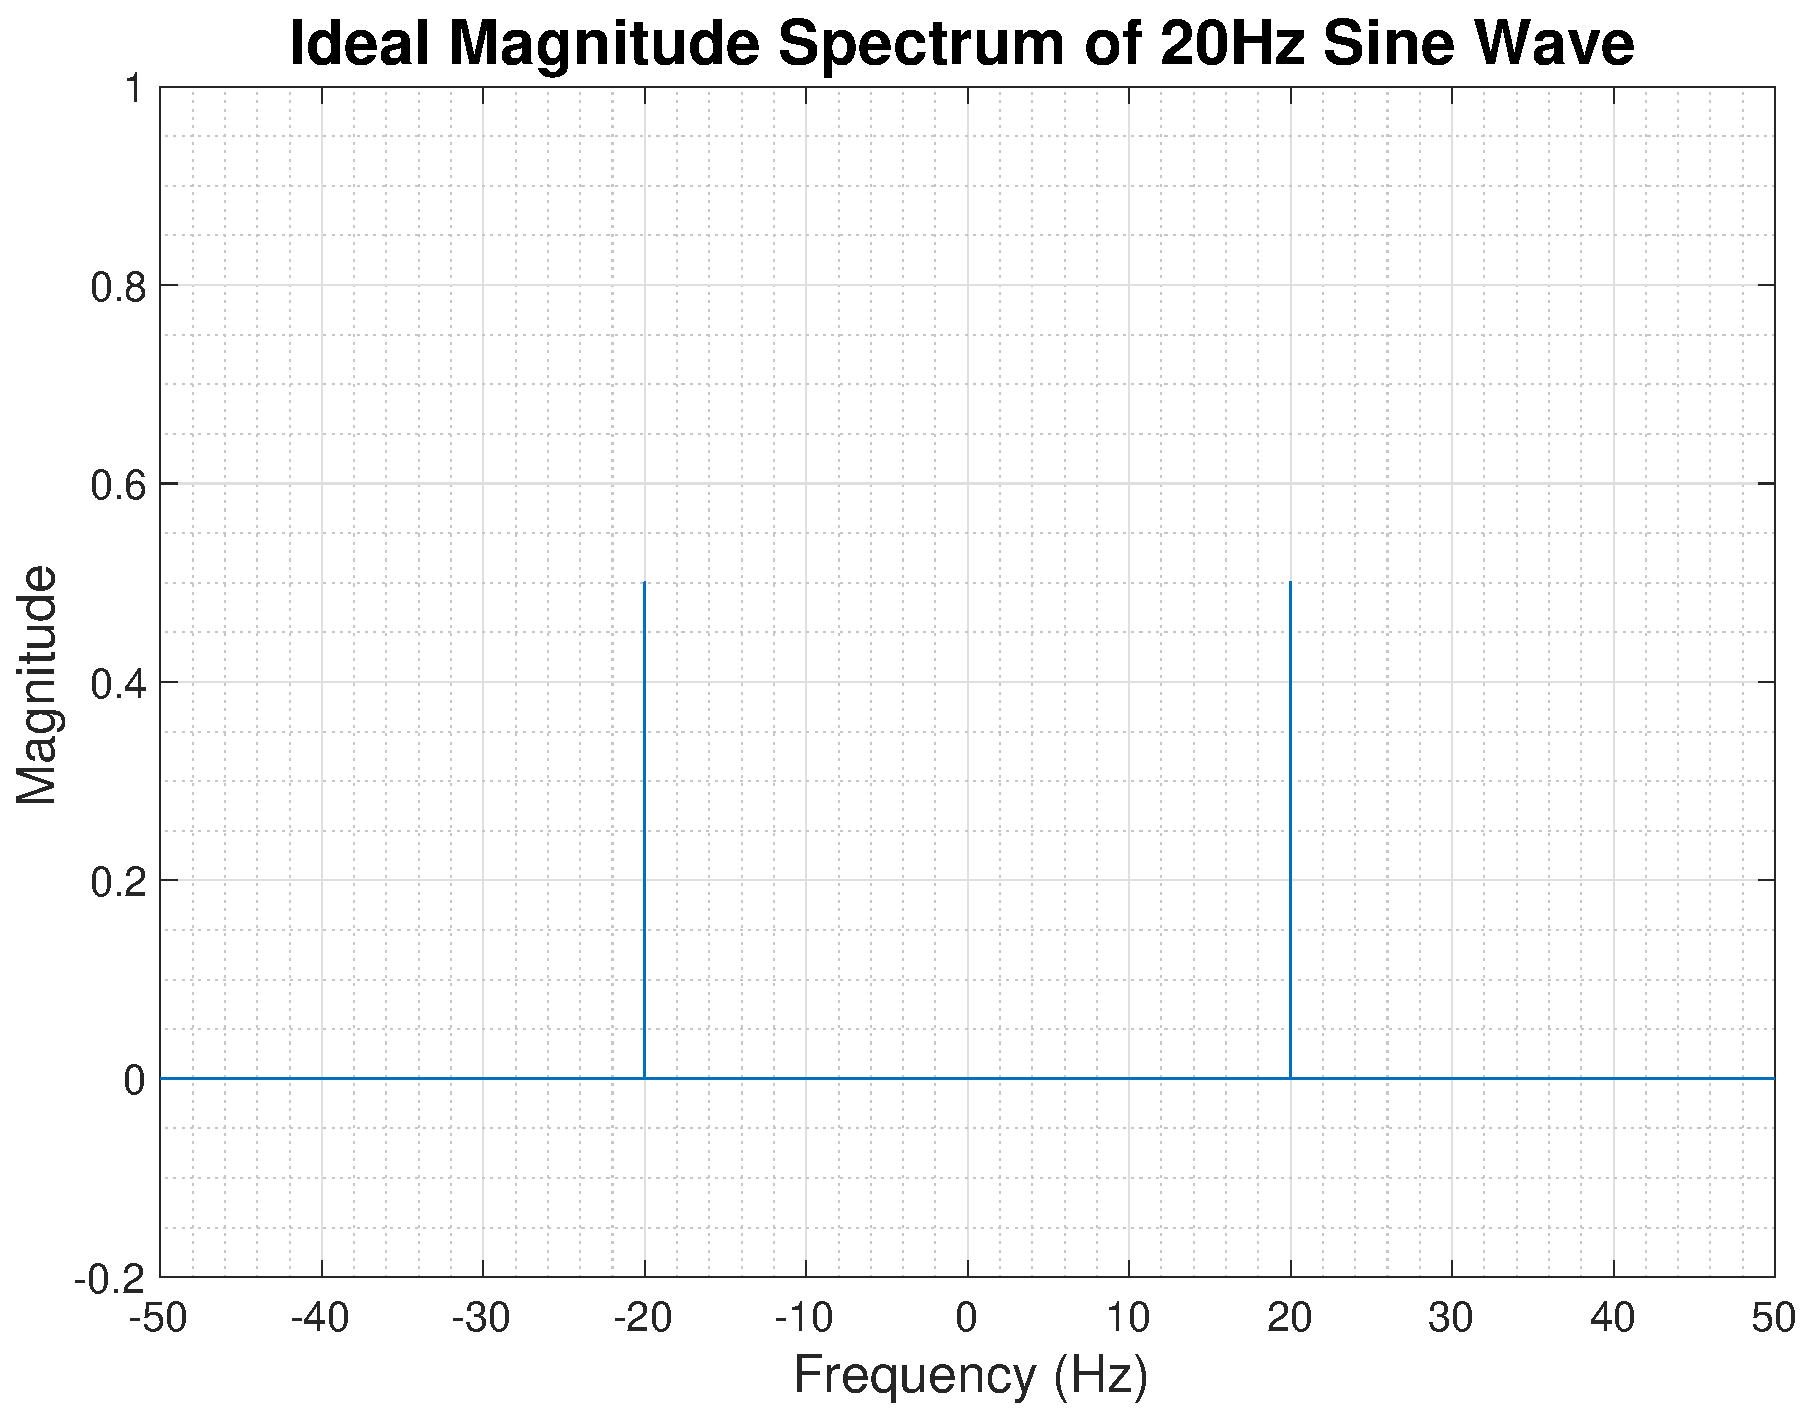
\includegraphics[width=0.32\textwidth]{part1/ideal_magnitude_spectrum_20hz_sine_wave}
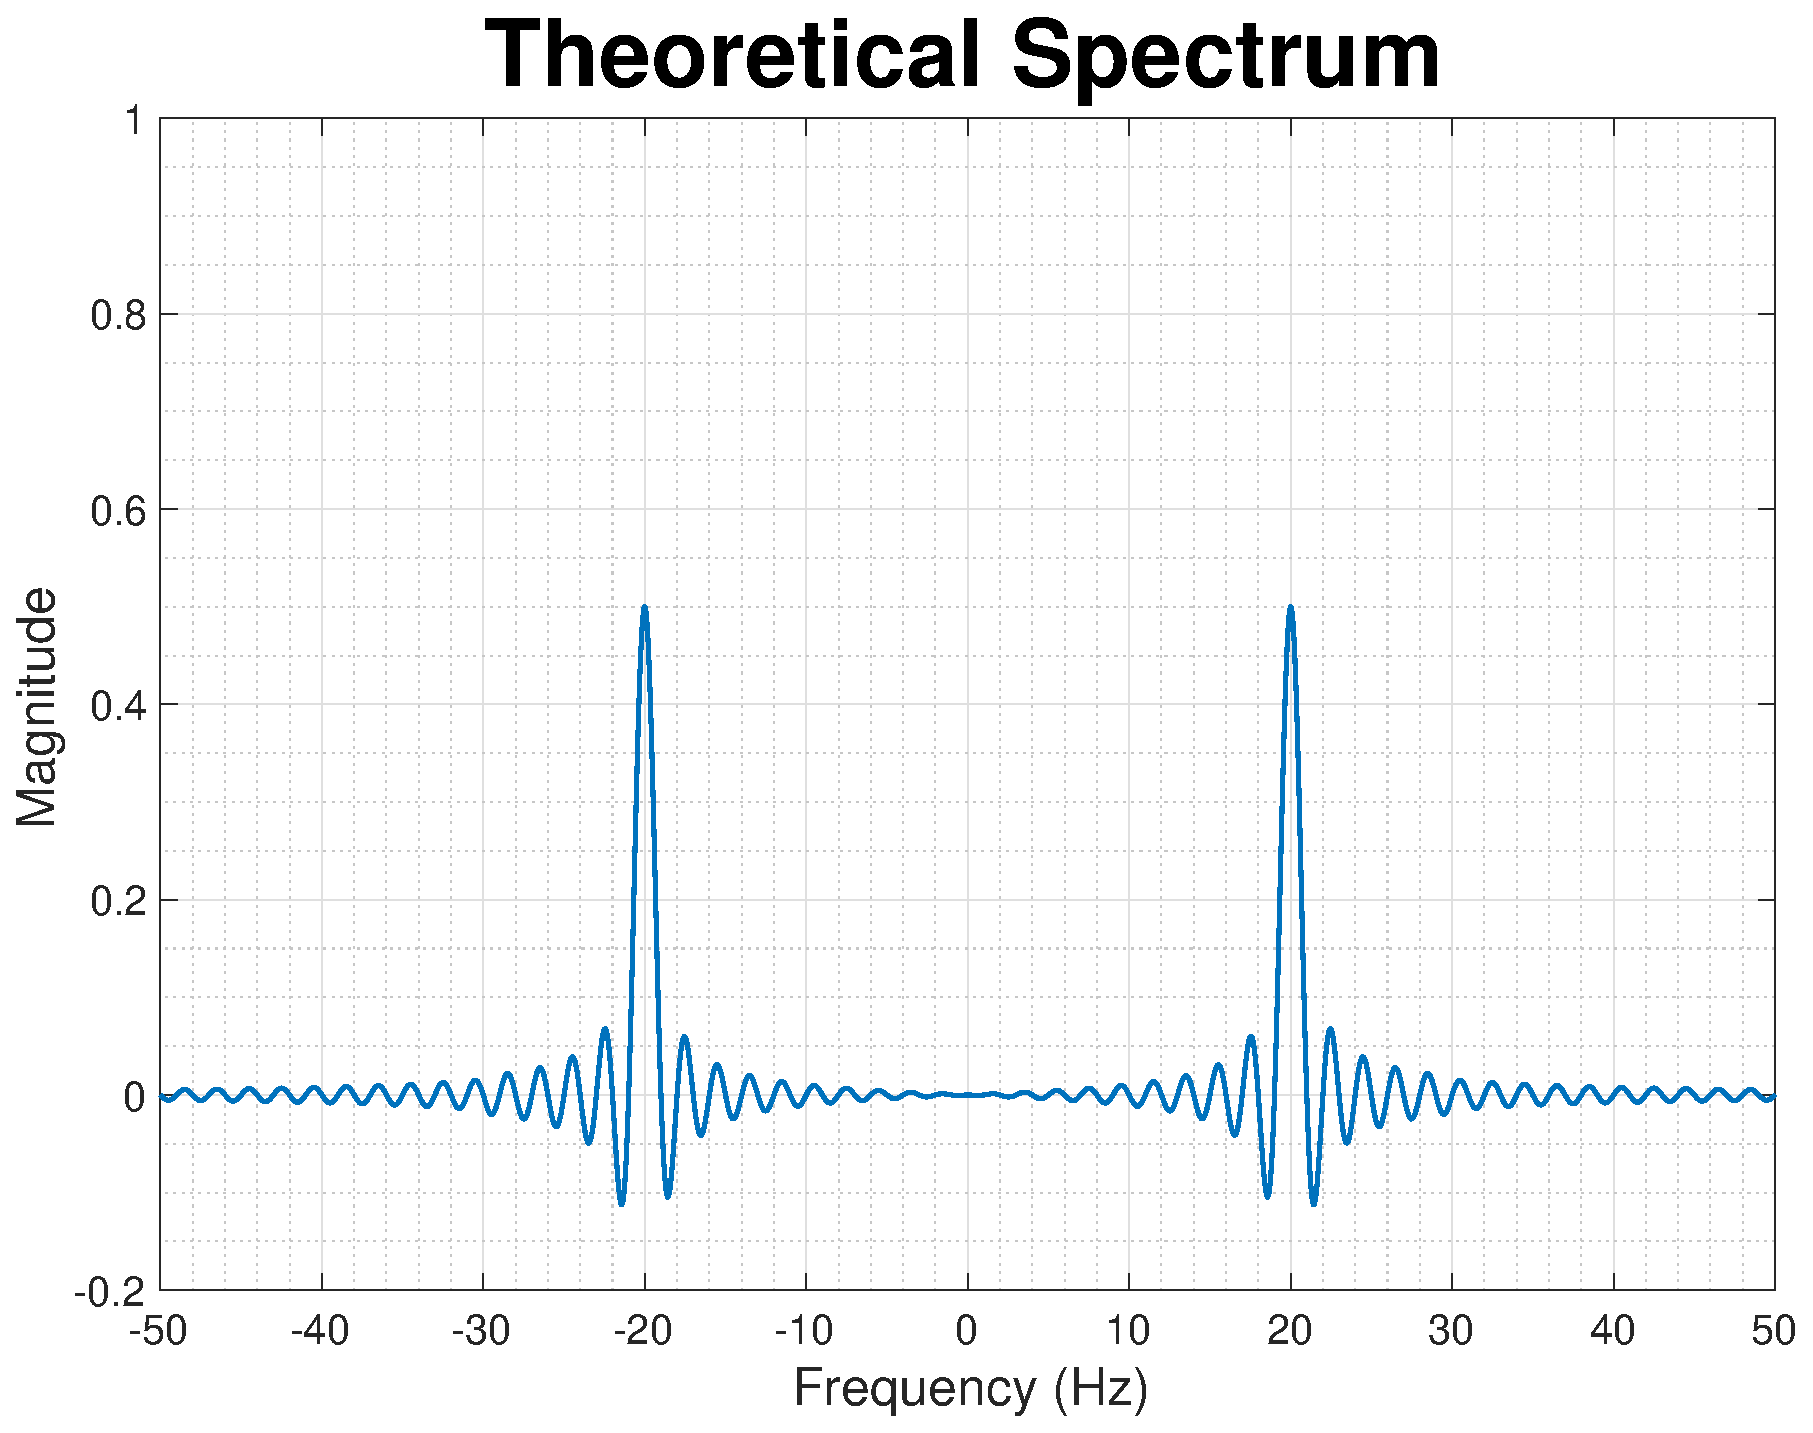
\includegraphics[width=0.32\textwidth]{part1/theoretical_magnitude_spectrum_windowed_20hz_sine_wave}
\caption{Ideal magnitude spectrum and Theoretical Continuous DTFT of 20 Hz sine wave}
\label{fig:ideal_and_theoretical_spectra_f_20}
\end{figure}

\noindent{}b. At first sight, it looks like the DFT spectrum on the left in Figure \ref{fig:dft_spectra_f_20} is exactly the same as ideal spectrum of a 20 Hz sine wave. However, we know that this cannot be the case. The ideal spectrum is derived from a continuous infinite duration sine wave whereas the spectra presented below are both derived from finite duration discrete-time sine waves. In fact, both the spectra below are sampled versions of the theoretical continuous magnitude spectrum shown in Figure \ref{fig:ideal_and_theoretical_spectra_f_20}. The resemblance described above comes from the fact that \textbf{coherent sampling} was performed. The rectangular window used to limit is signal is 0.1 s long and thus the \textit{sinc} function will have intercepts at integer interval of $f=\frac{1}{0.1}=10 Hz$. 100 samples are evenly divided across an axis that is 1000 Hz long and thus, each sample is separated by 10 Hz and exactly corresponds to frequencies at which the \textit{sinc} function is 0, expect of course at $\pm 20$ Hz. The spectral smearing and leakage artifacts that come about from time limiting the signal with a rectangular window become evident when more points from the continuous spectrum are sampled. This is clear by studying the graph on the right in Figure \ref{fig:dft_spectra_f_20}.

\begin{figure}[H]
\centering{}
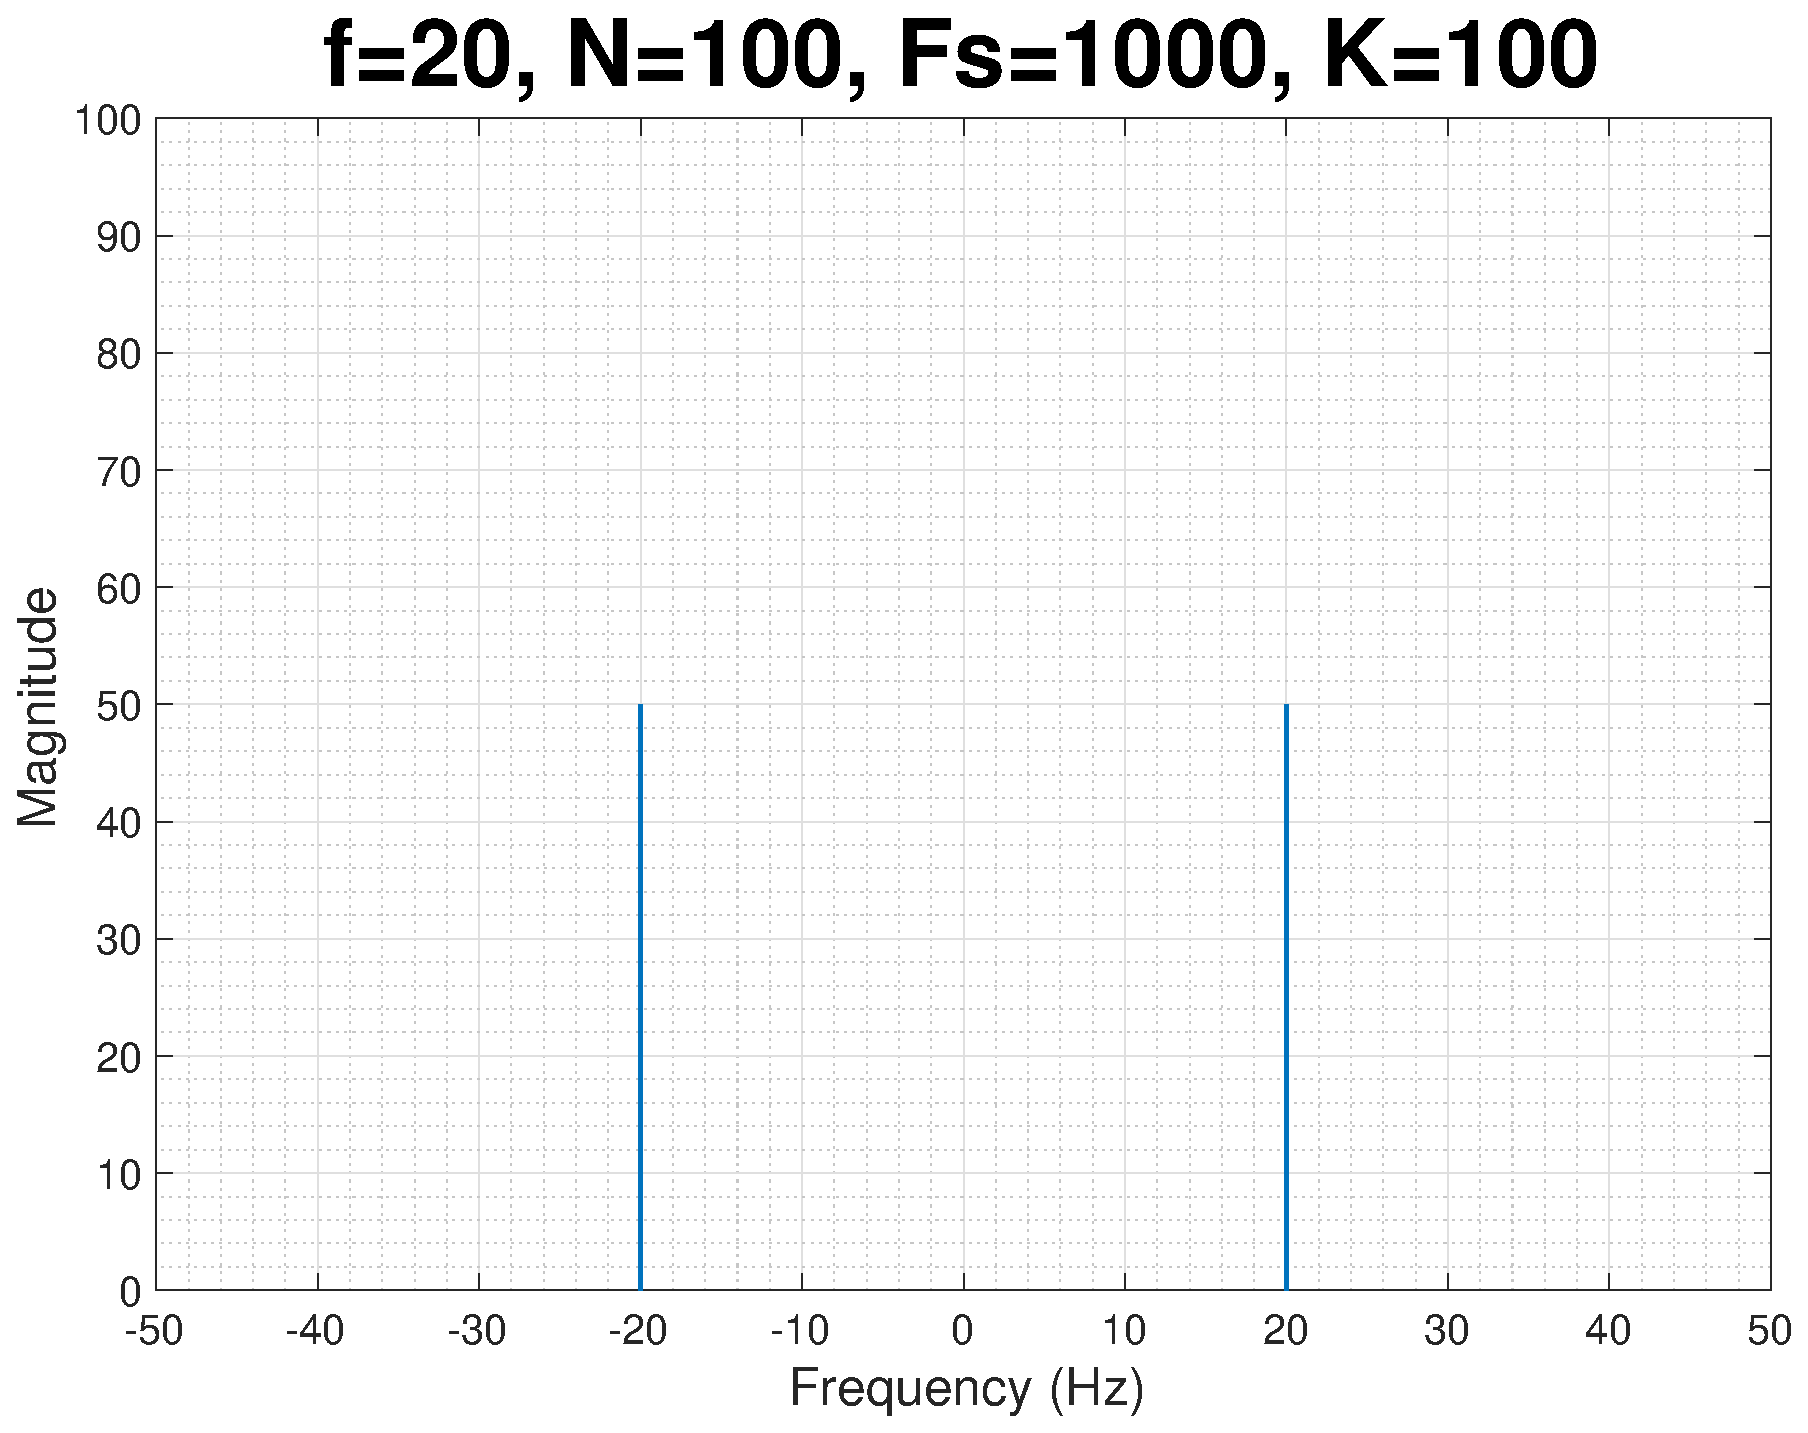
\includegraphics[width=0.32\textwidth]{part1/dft_spectra_f_20_n_100_Fs_1000_k_100}
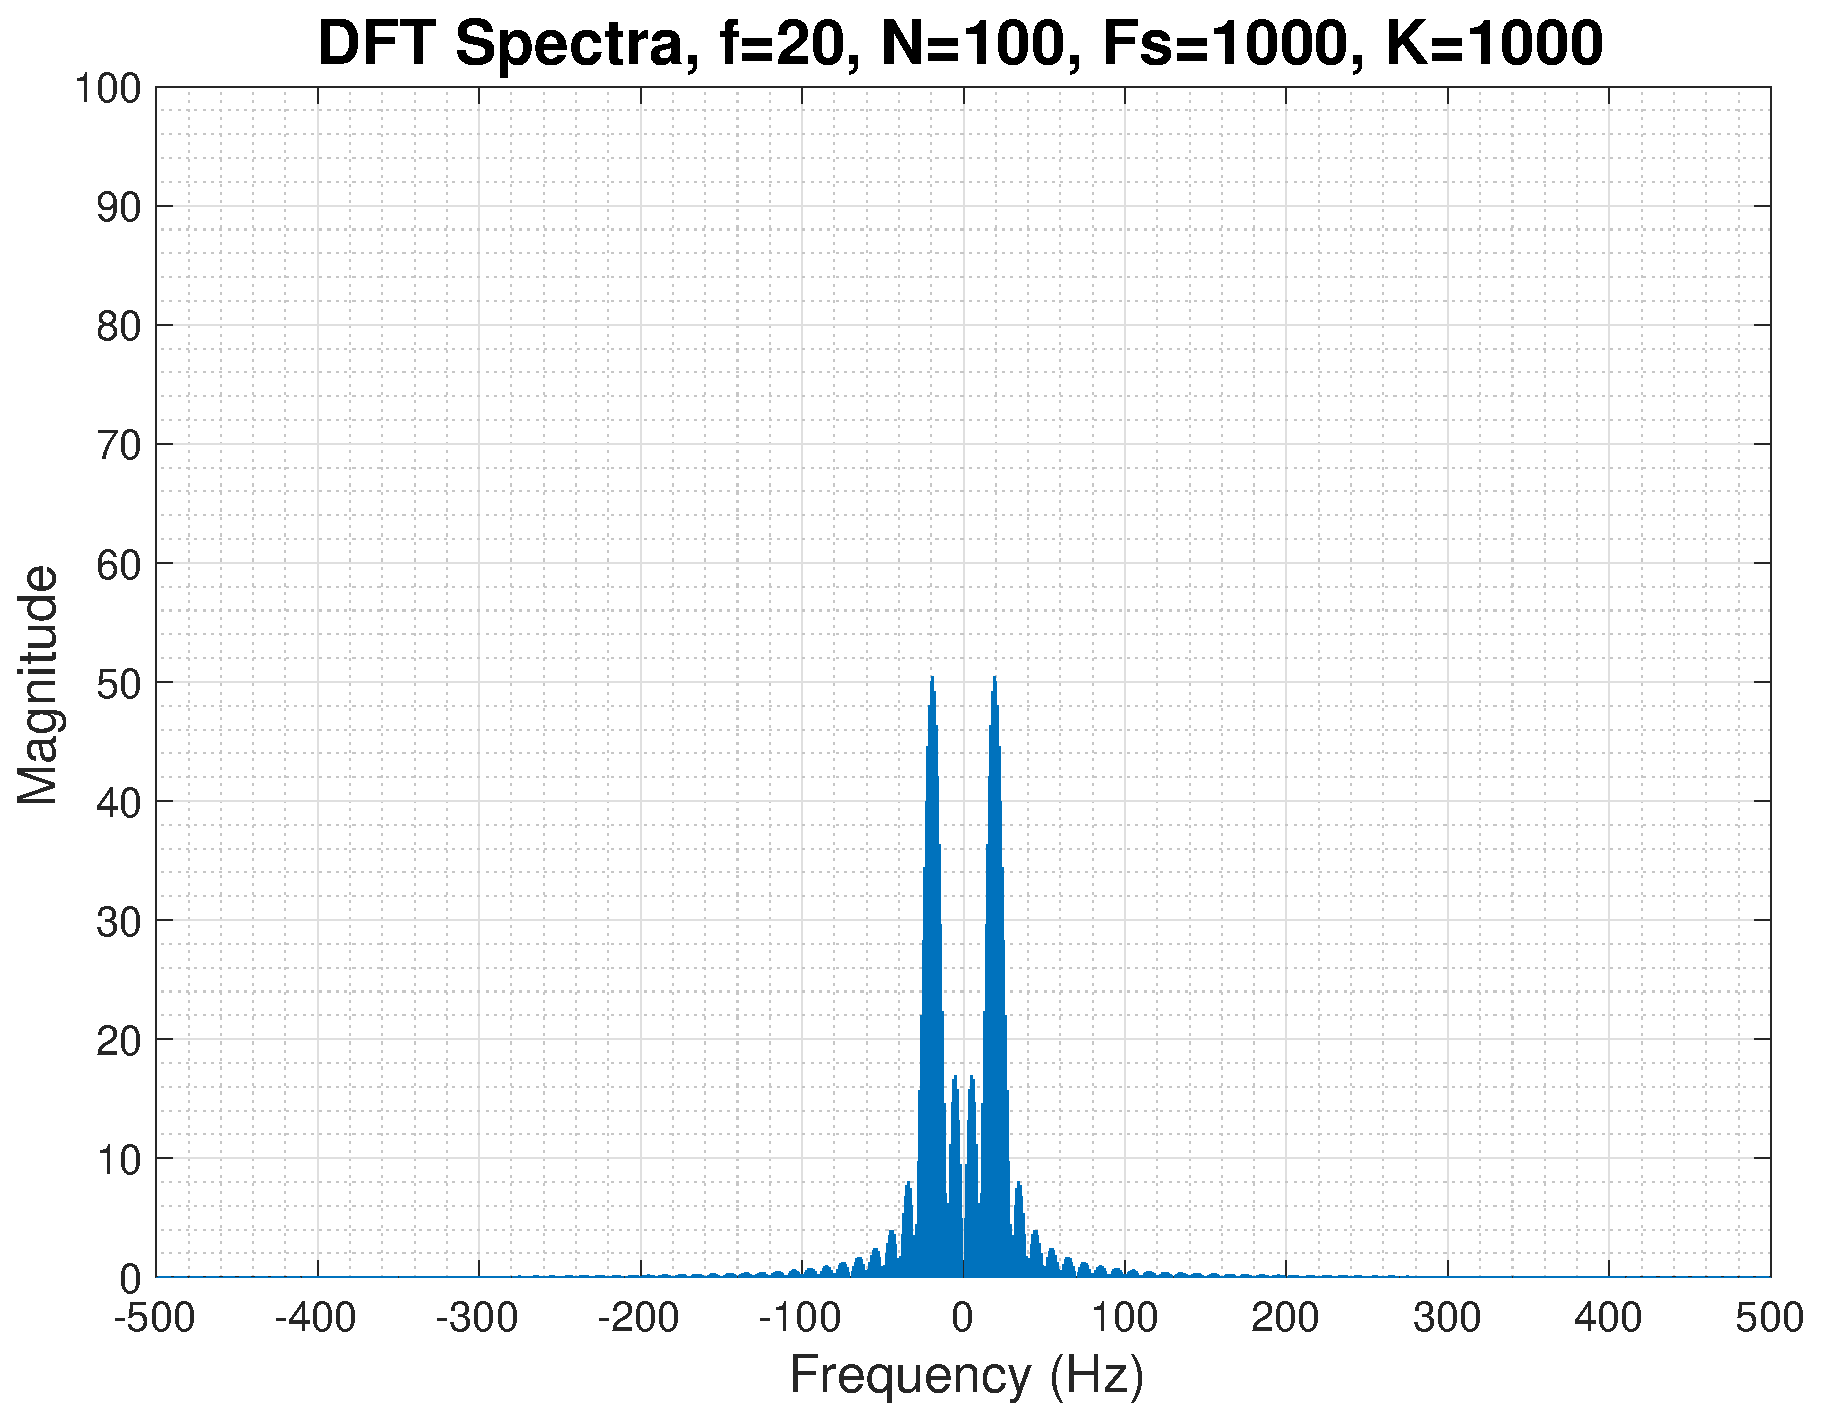
\includegraphics[width=0.32\textwidth]{part1/dft_spectra_f_20_n_100_Fs_1000_k_1000}
\caption{100 and 100 Point DFT Spectra of 20 Hz Sine Wave}
\label{fig:dft_spectra_f_20}
\end{figure}

\noindent{}c. The graphs in Figure \ref{fig:incoherent_sampling} show the K-point DFT spectra for $K=100$ and $K=2^{16}$; the graph on the right was generated using the \texttt{plot} function rather than the \texttt{stem} function since the theoretical spectra has been sampled so densely that it can be interpreted as effectively continuous. The graphs below illustrate the effects of sampling the continuous DTFT sparsely; the true peaks are not correctly identified. In fact, the peaks occur at bin $\frac{f_{R}}{f_{s}}=\frac{f x N}{f_{s}}=\frac{24*100}{1000}=2.4$; since this bin does not exist in the 100-point DFT spectrum, the peak at 24 Hz cannot be identified. Increasing the value of K can be used to solve the incoherent sampling problem. This is easily obtained by zero-padding the signal.

\begin{figure}[H]
\centering{}
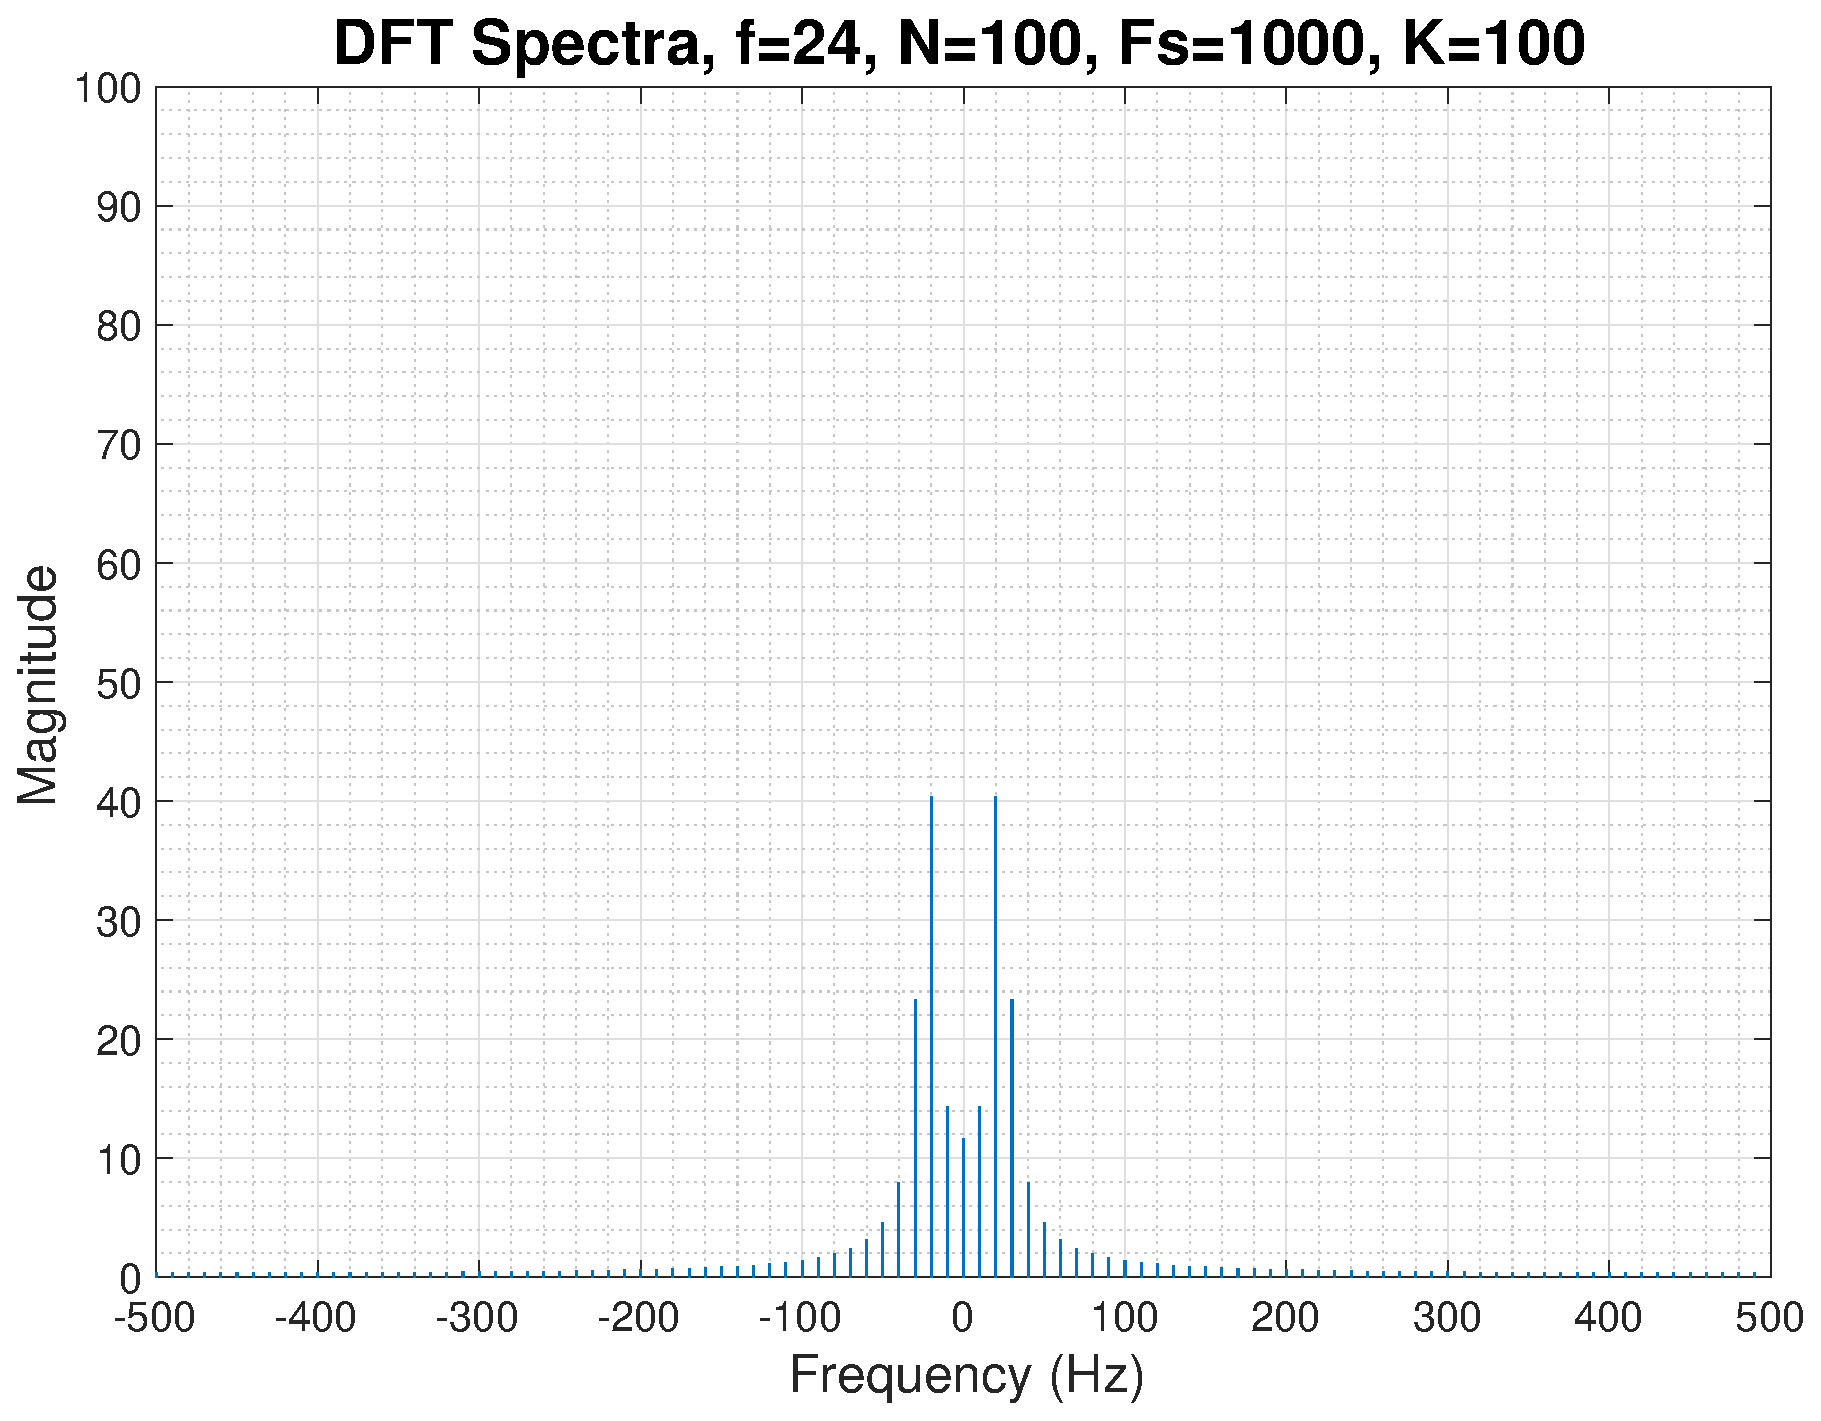
\includegraphics[width=0.32\textwidth]{part1/dft_spectra_f_24_n_100_Fs_1000_k_100}
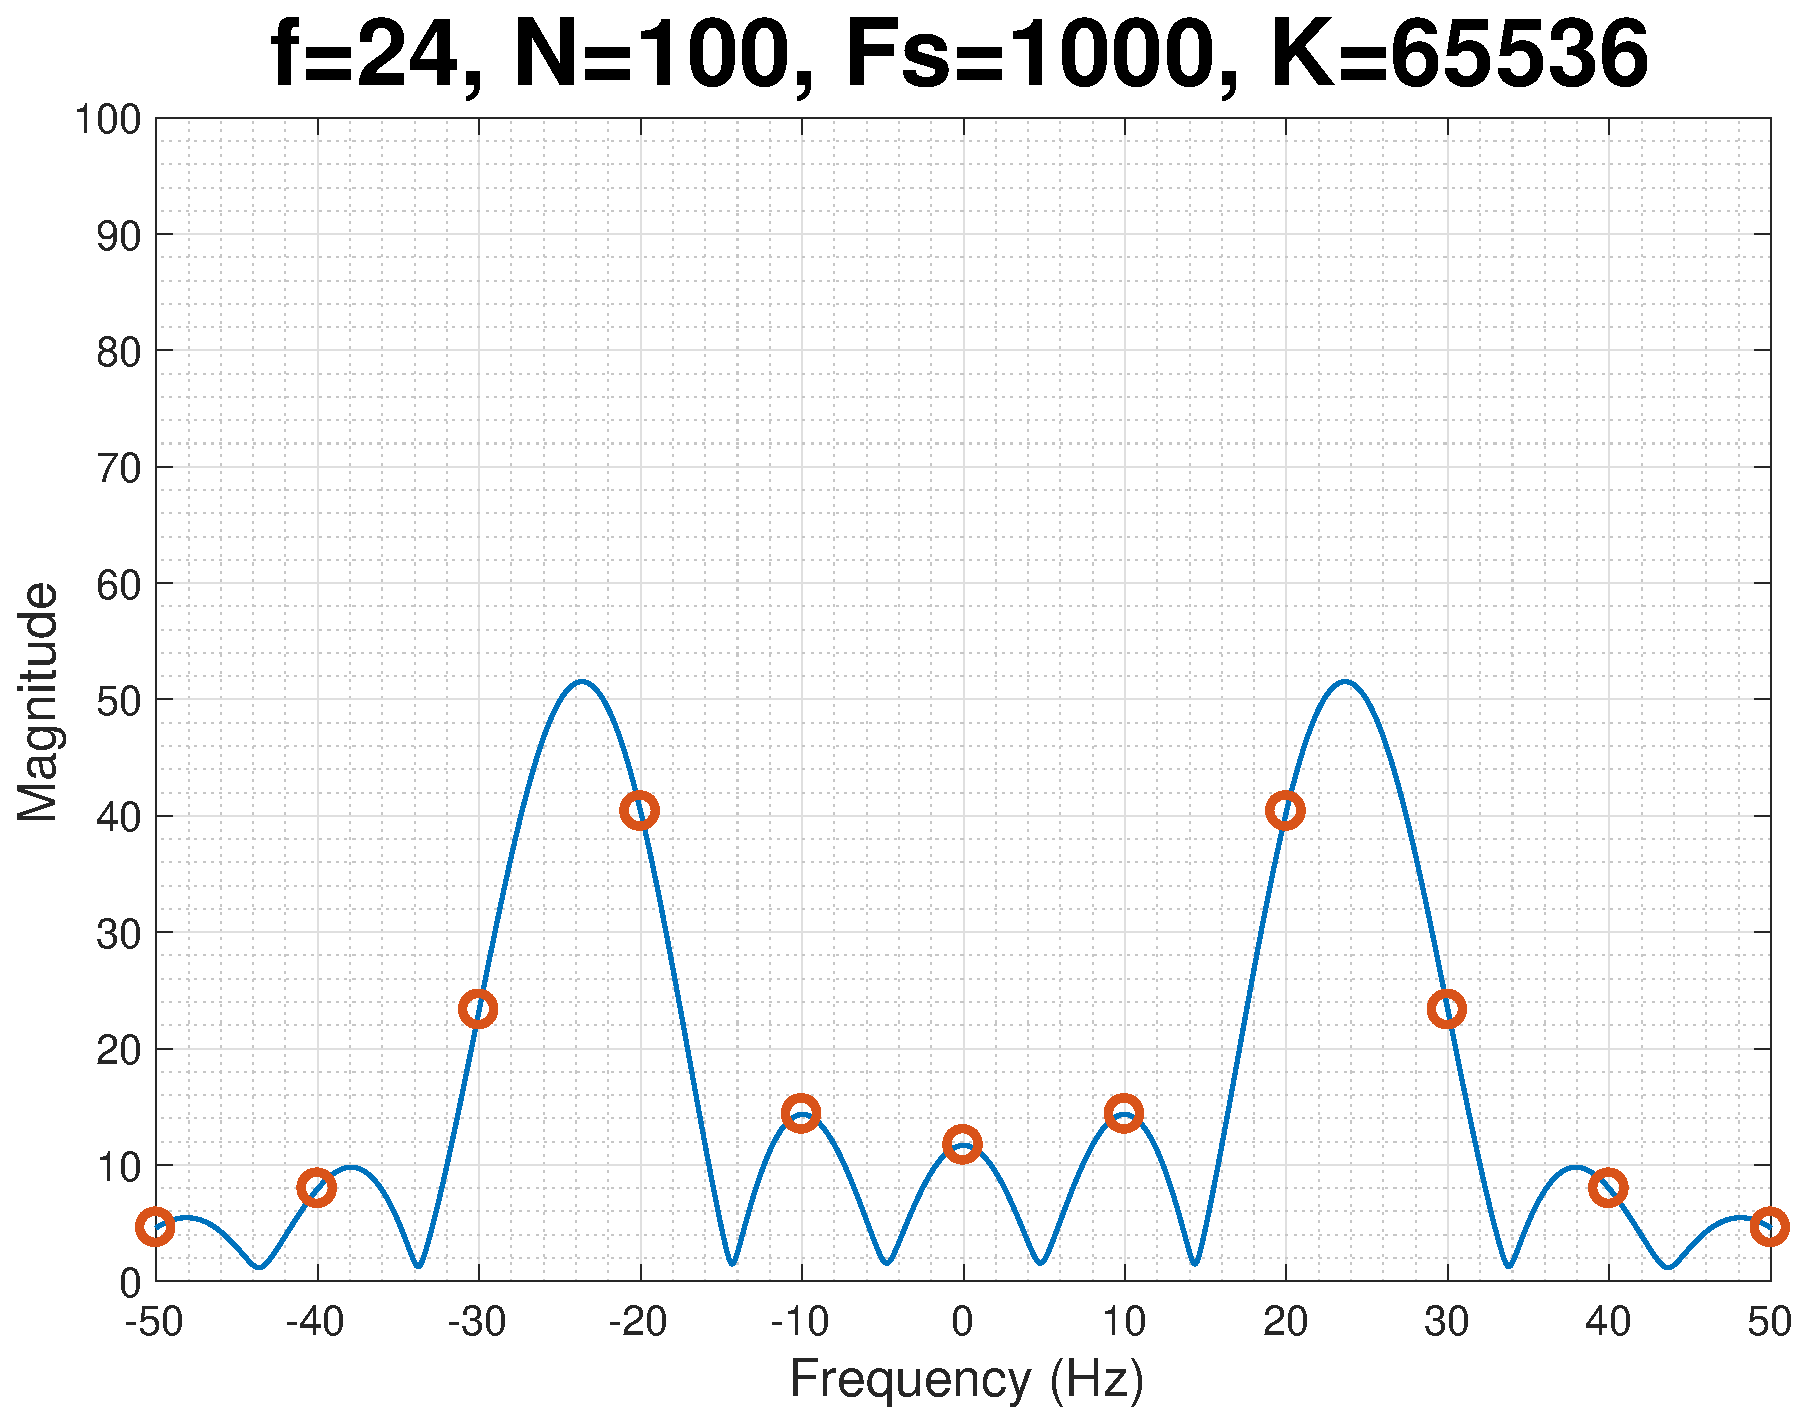
\includegraphics[width=0.32\textwidth]{part1/dft_spectra_f_24_n_100_Fs_1000_k_2_to_16}
\caption{DFT Spectra Illustrating the Effects of Incoherent Sampling}
\label{fig:incoherent_sampling}
\end{figure}

\subsection{Properties of Power Spectral Density (PSD)}

\subsubsection*{Approximation in the definition of PSD}

\noindent{}To show the equivalence of the two equations I shall start with (\ref{eq:psd_expectation}).

\begin{align}
P(\omega)	&=\lim_{N \to \infty} E \Bigg\{ \frac{1}{N} \Bigg\lvert\sum_{n=0}^{N-1} x(n)e^{-jn\omega}\Bigg\rvert^{2} \Bigg\} \label{eq:psd_expectation} \\
			&=\lim_{N \to \infty} E \Bigg\{ \frac{1}{N} \sum_{m=0}^{N-1} x(m)e^{-jm\omega}\sum_{n=0}^{N-1} x^{*}(n)e^{jn\omega} \Bigg\} \nonumber \\
			&=\lim_{N \to \infty} \frac{1}{N} \sum_{m=0}^{N-1} \sum_{n=0}^{N-1} E \Bigg\{x(m)x^{*}(n)\Bigg\} e^{-jm\omega}e^{jn\omega} \nonumber \\
			&=\lim_{N \to \infty} \frac{1}{N} \sum_{m=0}^{N-1} \sum_{n=0}^{N-1} r_{xx}(m-n) e^{-j(m-n)\omega} \nonumber			
\end{align}

\noindent{}Substituting $\tau=m-n$ and incorporating the double summation into one summation, we get:

\begin{align}
P(\omega)	&=\lim_{N \to \infty} \frac{1}{N} \sum_{\tau=-N+1}^{N-1}  (N-\lvert \tau \rvert) r_{xx}(\tau) e^{-j\tau\omega} \nonumber \\
			&=\sum_{\tau=-\infty}^{\infty}r(\tau)e^{-j\tau\omega} - \lim_{N \to \infty} \frac{1}{N} \sum_{\tau=-N+1}^{N-1} \lvert \tau \rvert r(\tau) e^{j\tau\omega} \nonumber
\end{align}

\noindent{}And thus under the mild assumption that the covariance sequence $r(k)$ decays rapidly we have shown that (\ref{eq:psd_expectation}) is equivalent to (\ref{eq:psd_dtft_acf}), which is simply the continuous DTFT of the Autocovariance Function (ACF).

\begin{align}
P(\omega)	&= \sum_{\tau=-\infty}^{\infty}r(\tau)e^{-j\tau\omega} \label{eq:psd_dtft_acf}
\end{align}  

\noindent{}a. The Fourier Transform (FT) of a real symmetrical signal will also be real and symmetrical; the symmetry in the FT is due to the signal being real whereas the fact that the imaginary component of the FT is zero is due to the symmetrical nature of the signal. Matlab's FFT algorithm assumes that the incoming signal is wrapped and thus the specific structure of $\textbf{x}$, described in the coursework, is necessary. In contrast to the zero-padding performed in Section \ref{sec:dft_basics}, here we pad zeros to the middle of the vector $\textbf{x}$ to preserve symmetry. It is important to note that in this specific scenario, zero-padding is actually the same as extending the duration for which we observe the signal; this is because for $|k|\geq M$, the autocovariance function is $0$. As such, zero-padding is increasing the frequency resolution of $P(\omega_{k})$. In contrast, zero-padding is usually used to increase the number of points for the which the continuous DTFT is sampled and the frequency resolution depends solely on the size of the rectangular window used to restrict the signal from an infinite duration to a finite duration. The graphs below clearly illustrate this point. It is interesting to note that the autocovariance function described in the coursework is actually the ACF of the rectangular window. As $M$ is increased from $10$ to $128$, the width of the mainlobe decreases; this is exactly what we expect. Smearing of the spectra is inversely proportional to the width of the rectangular window.

\begin{figure}[H]
\centering{}
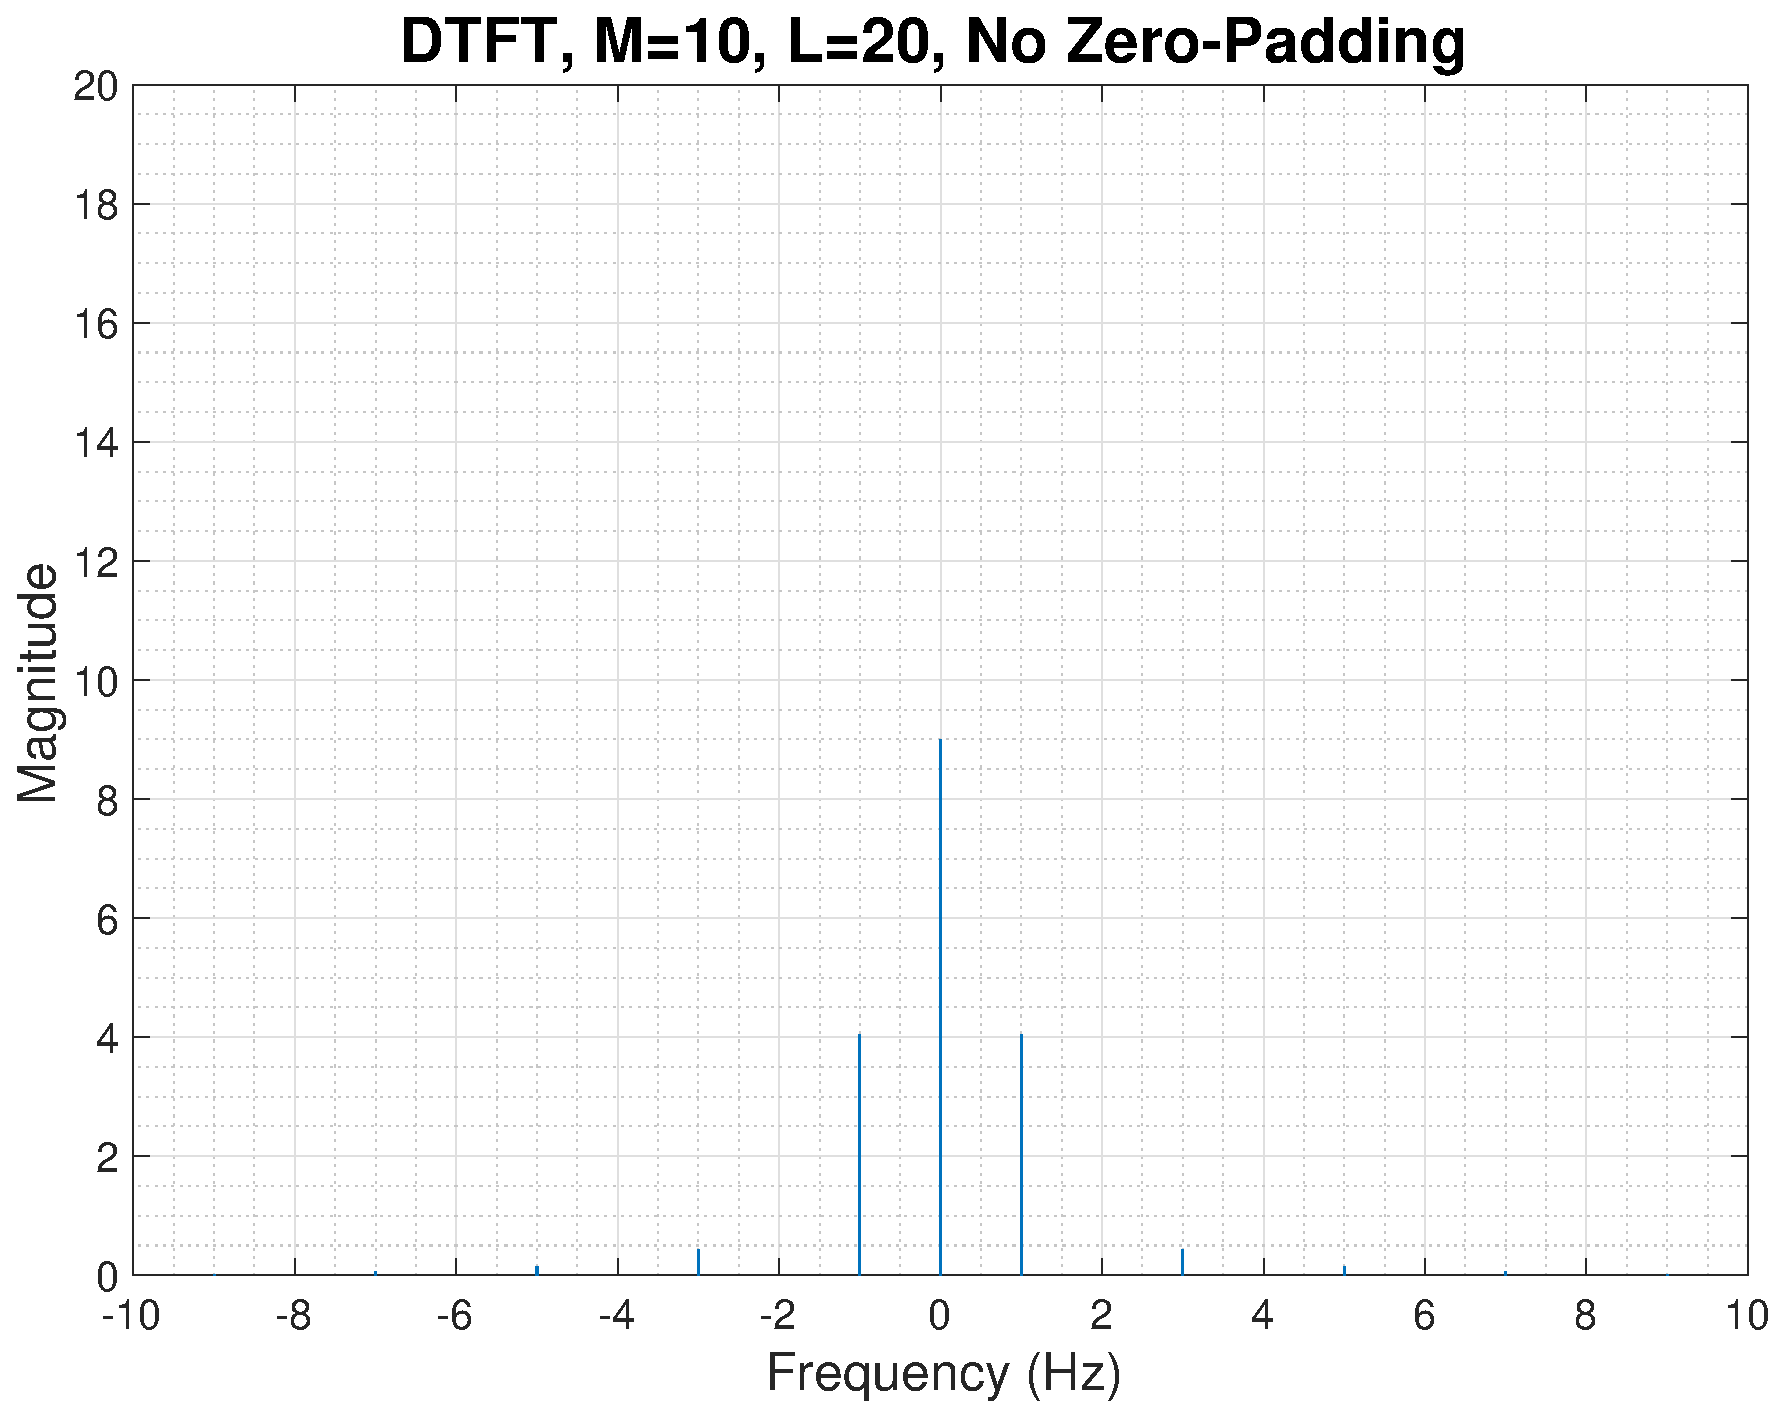
\includegraphics[width=0.32\textwidth]{part1/dft_spectra_acf_m_10_l_20}
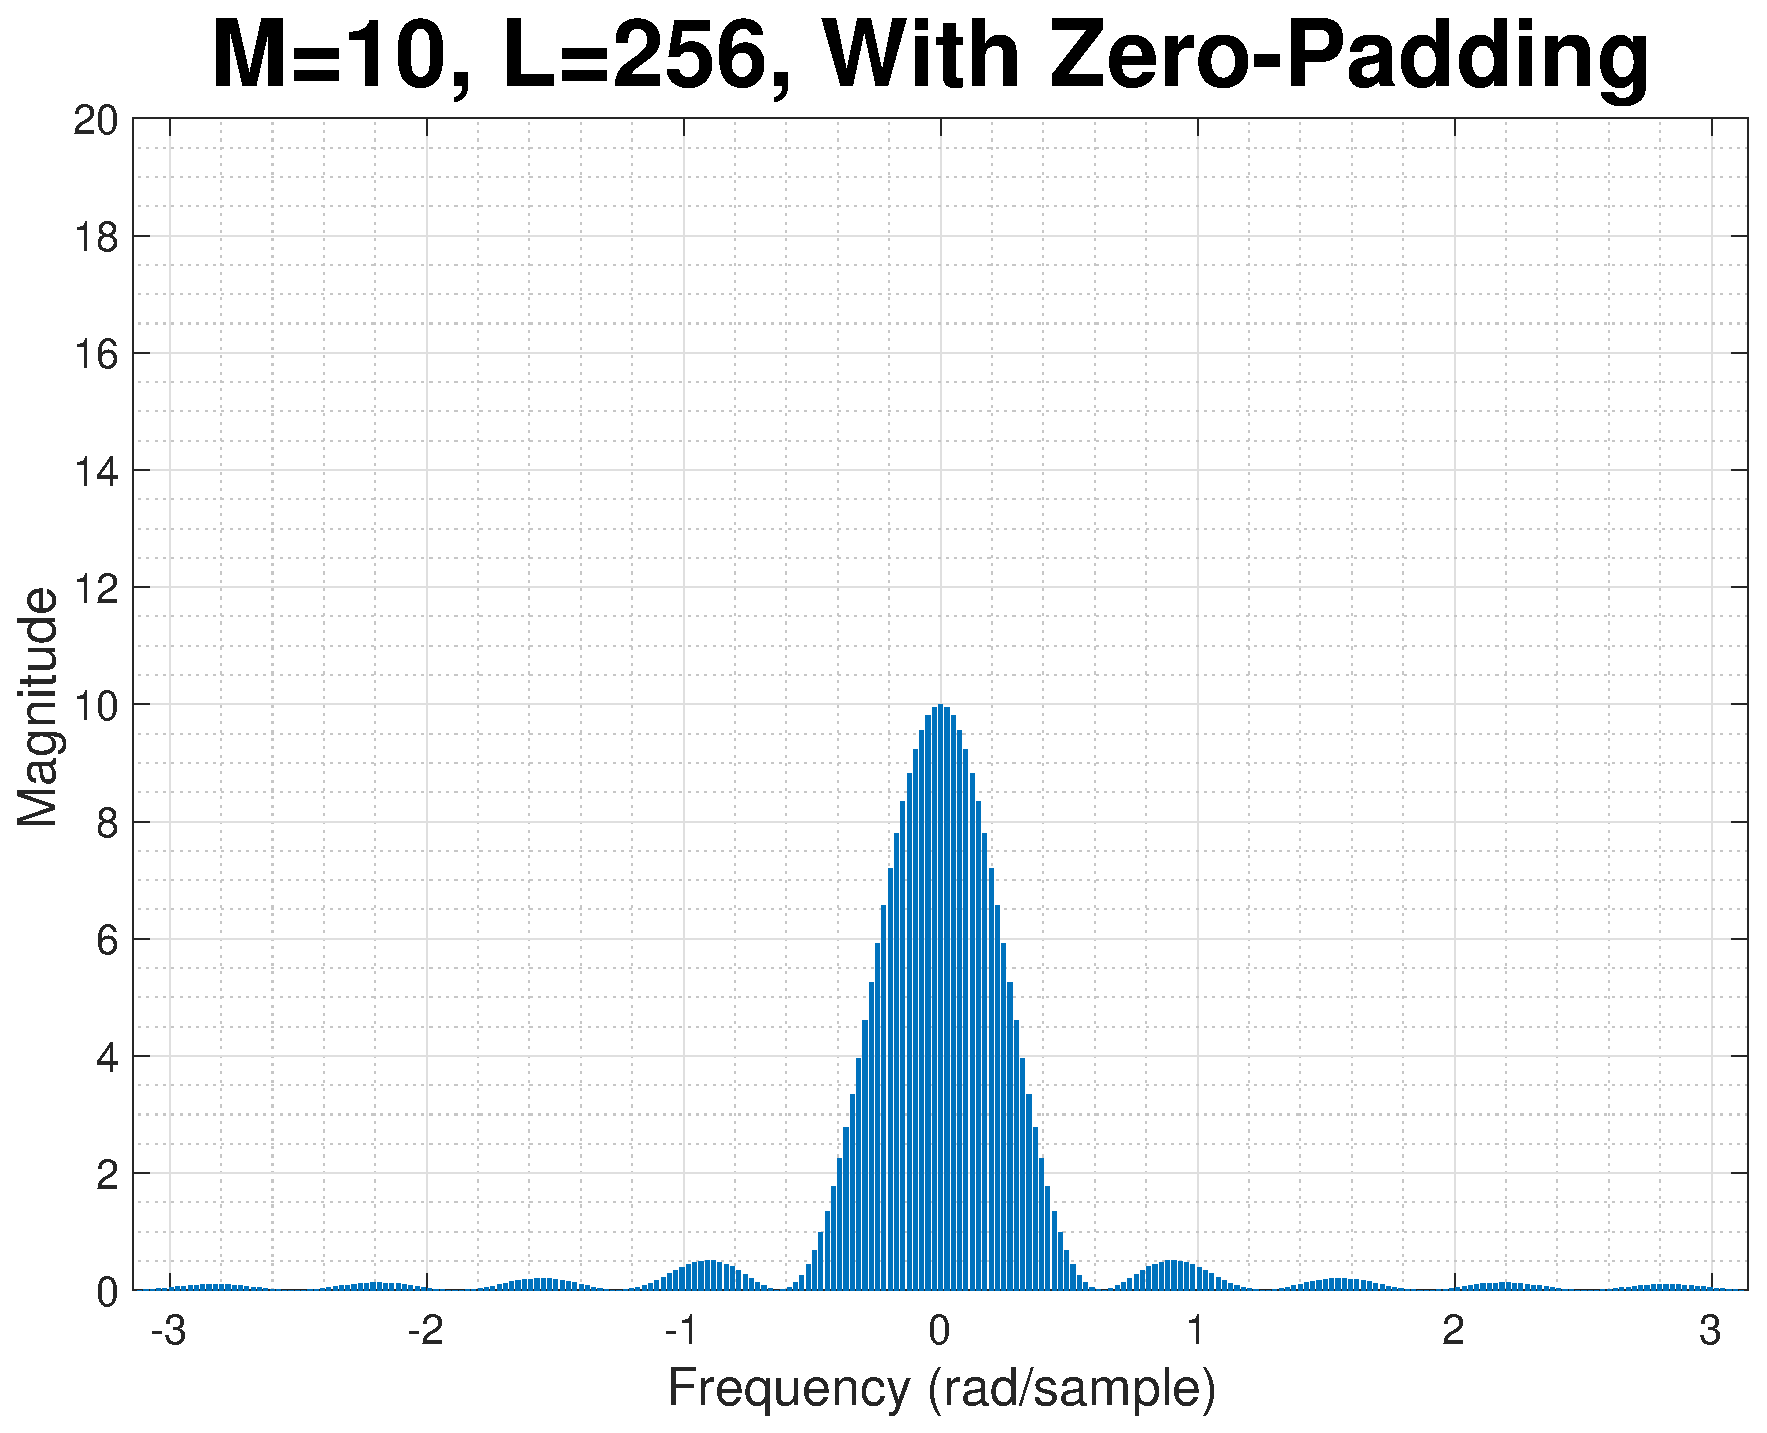
\includegraphics[width=0.32\textwidth]{part1/dft_spectra_acf_m_10_l_256} \\
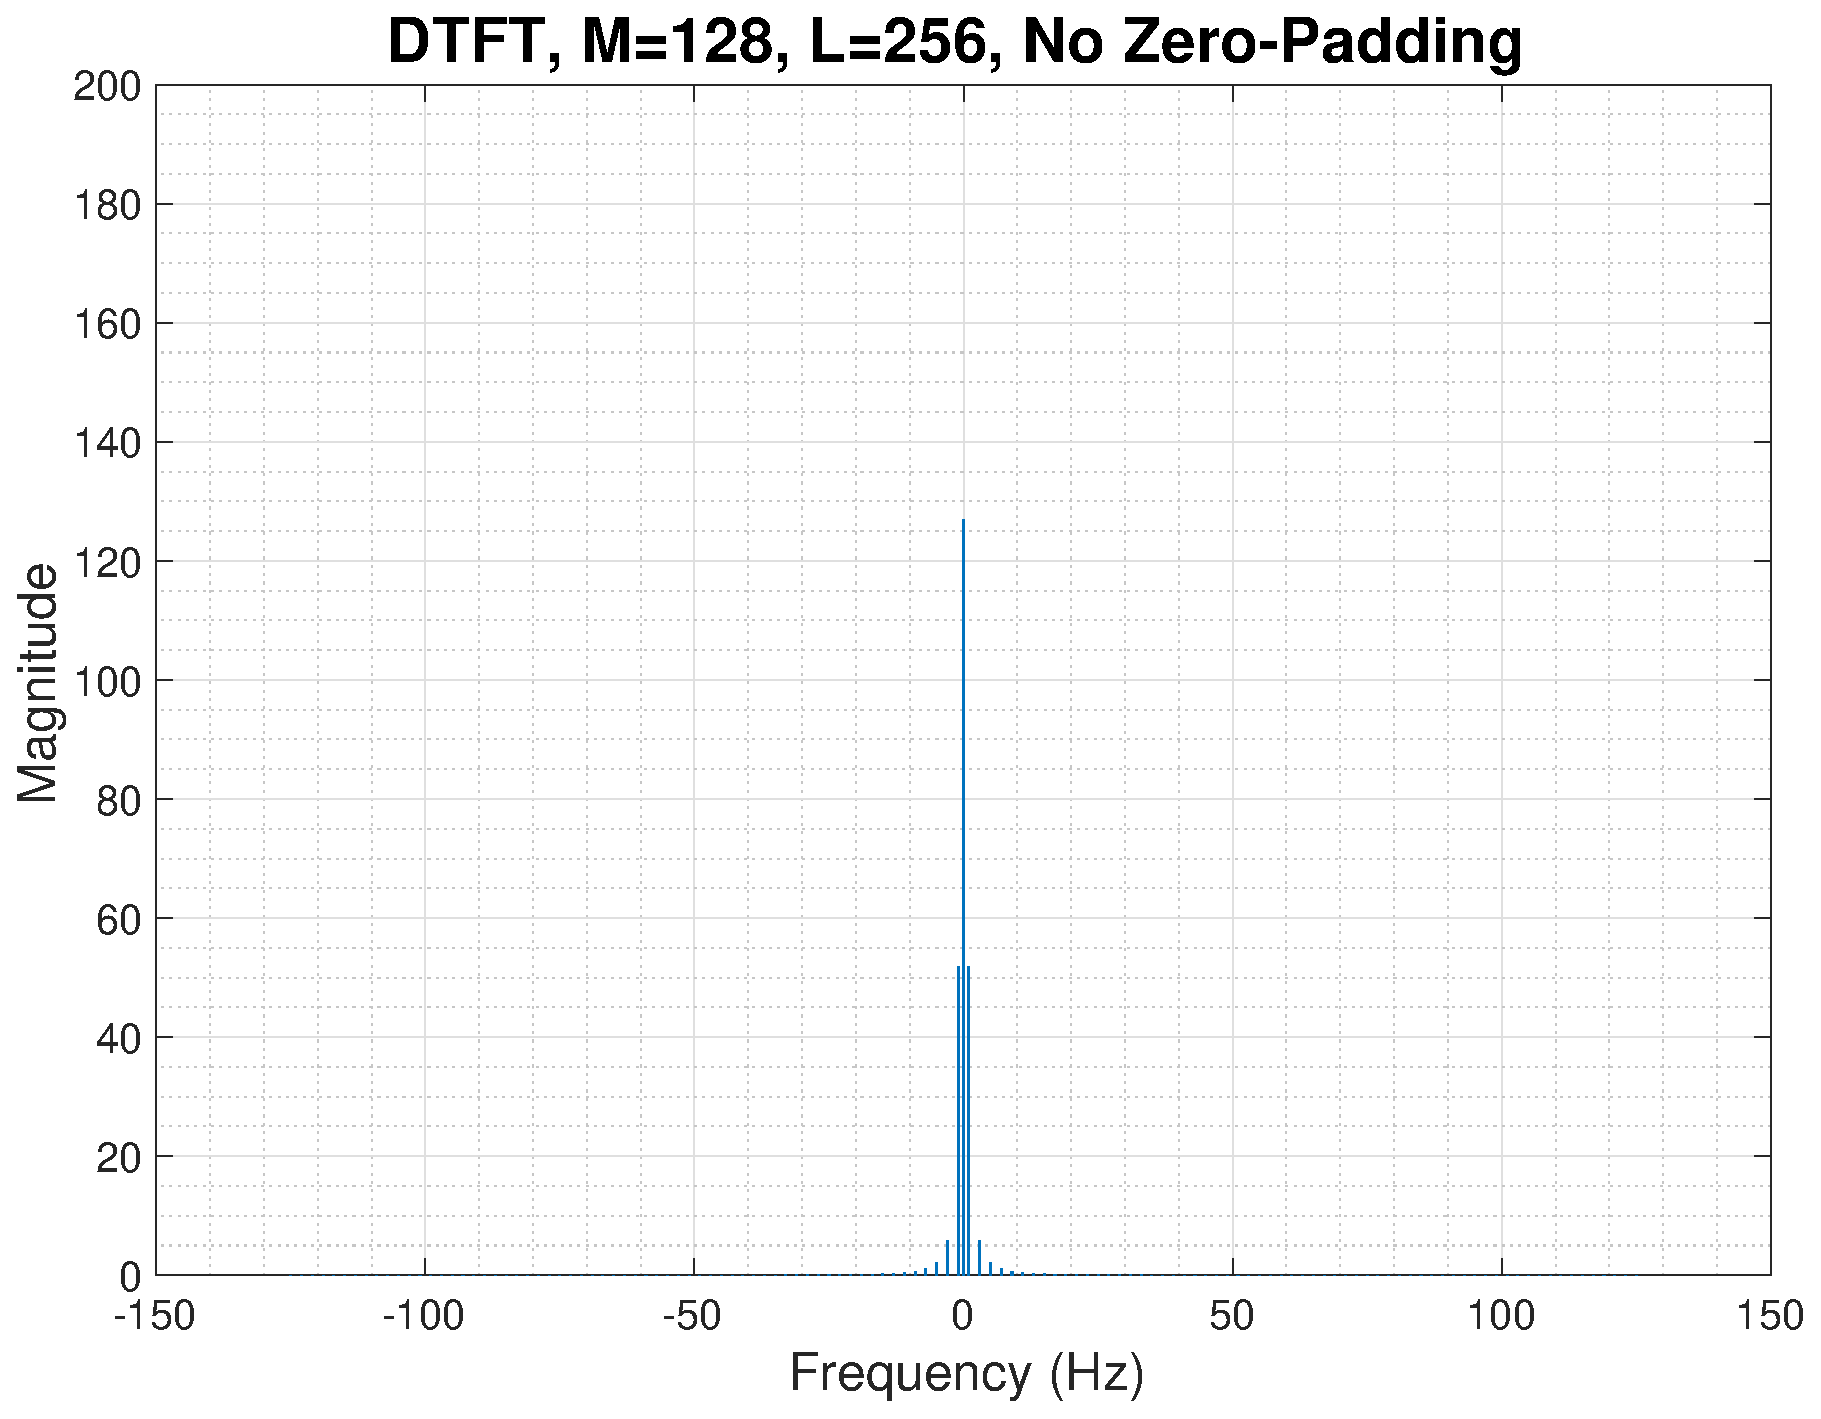
\includegraphics[width=0.32\textwidth]{part1/dft_spectra_acf_m_128_l_256}
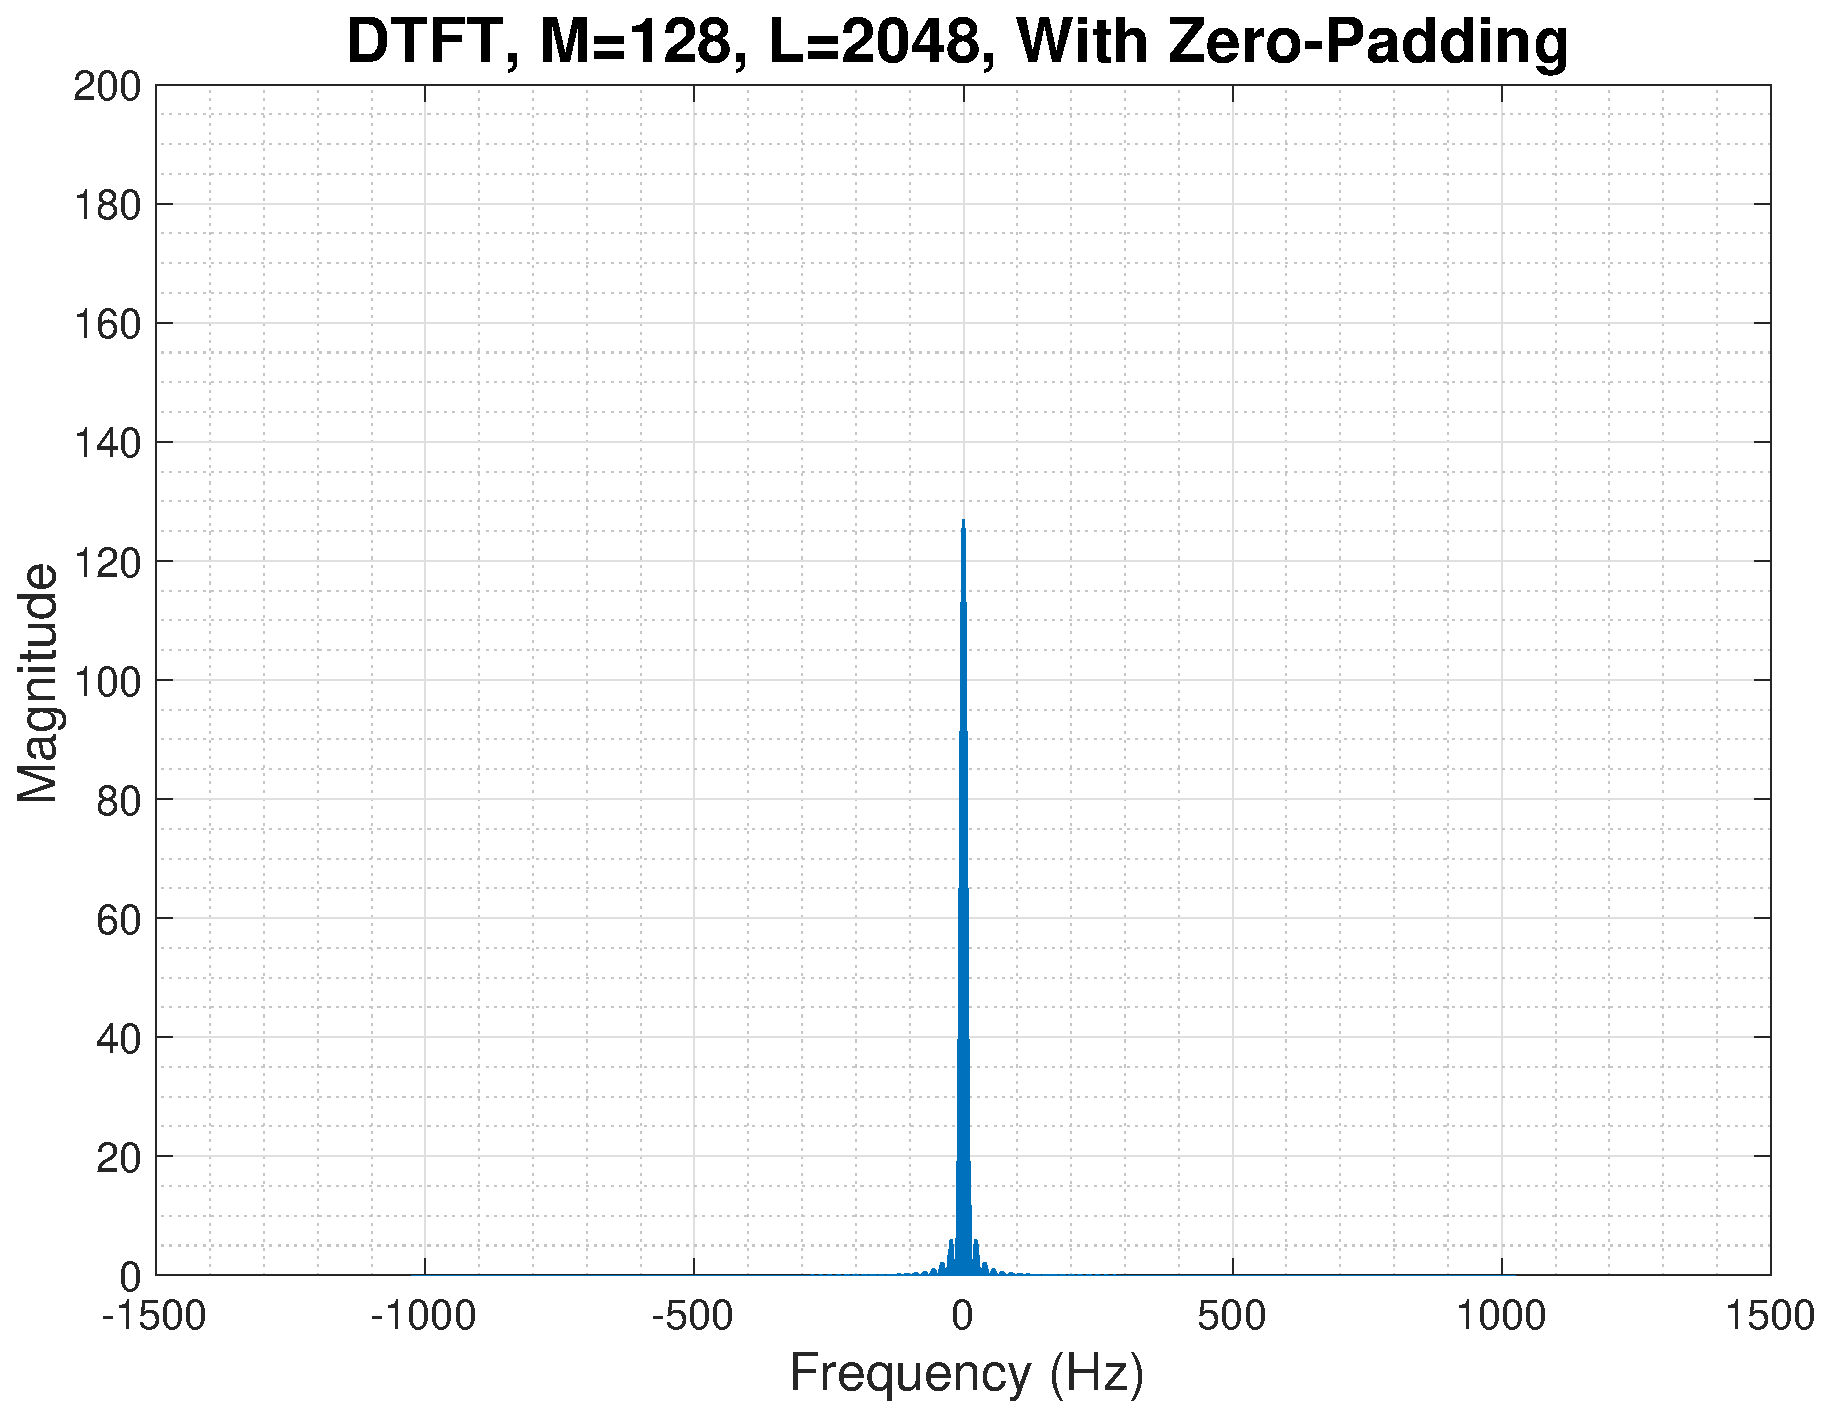
\includegraphics[width=0.32\textwidth]{part1/dft_spectra_acf_m_128_l_2048}
\caption{$P(\omega_{k})$ of $r(k)$ Described in the Coursework with and without Zero-Padding for $M=10$ and $M=100$}
\end{figure}

\noindent{}b. Due to the symmetrical nature of the signal for which we are taking the FFT, we do not expect any imaginary components. The graph below shows that the imaginary components are extremely small and are about $15$ orders of magnitude smaller than the real components. Above, the \texttt{abs} function was used to eliminate the imaginary components. Using the \texttt{real} function had no significant difference due to the extremely small values for the imaginary components.

\begin{figure}[H]
\centering{}
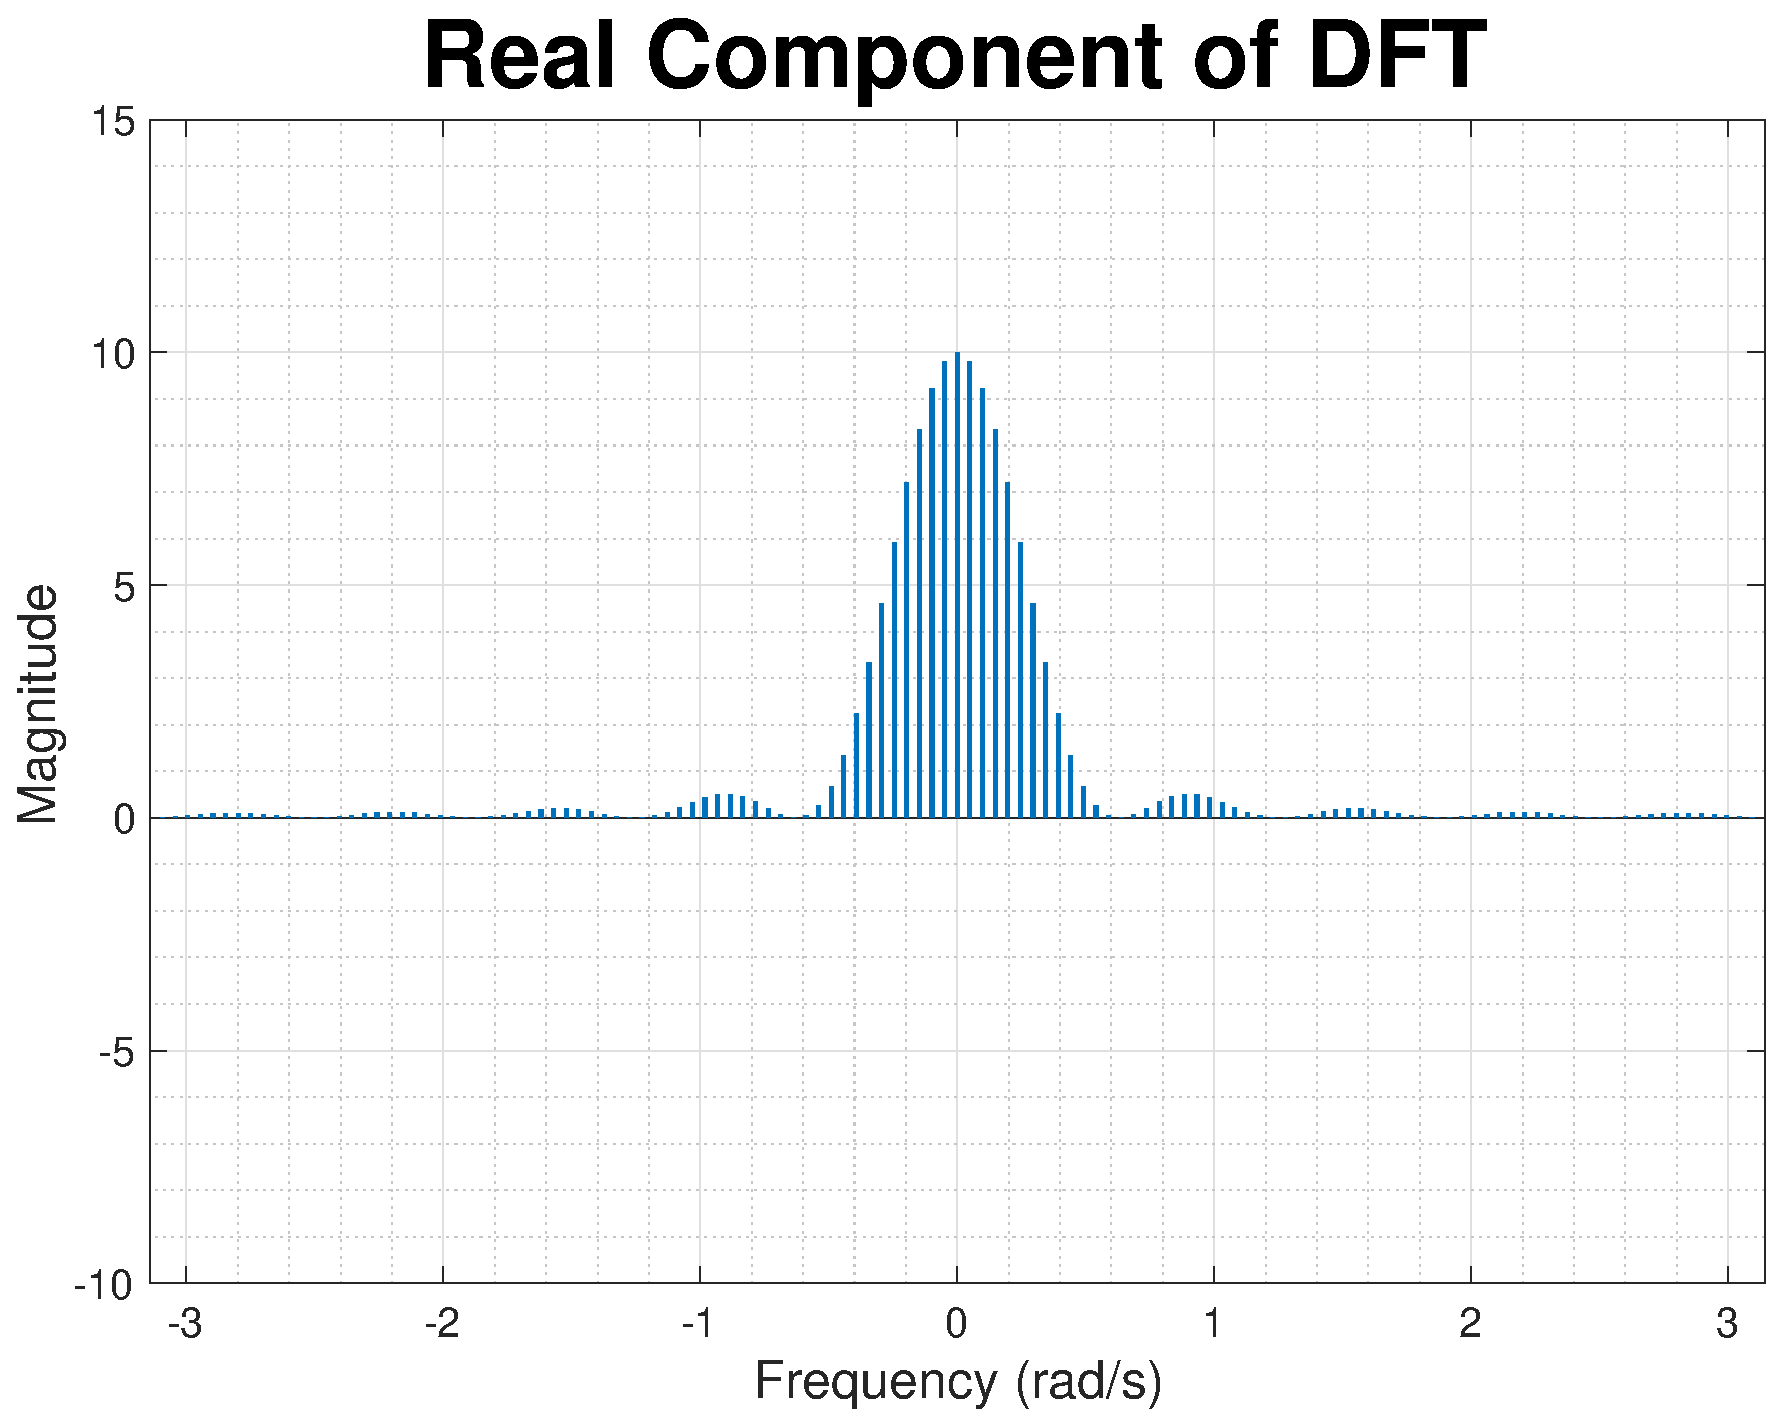
\includegraphics[width=0.32\textwidth]{part1/dft_spectra_acf_x_real}
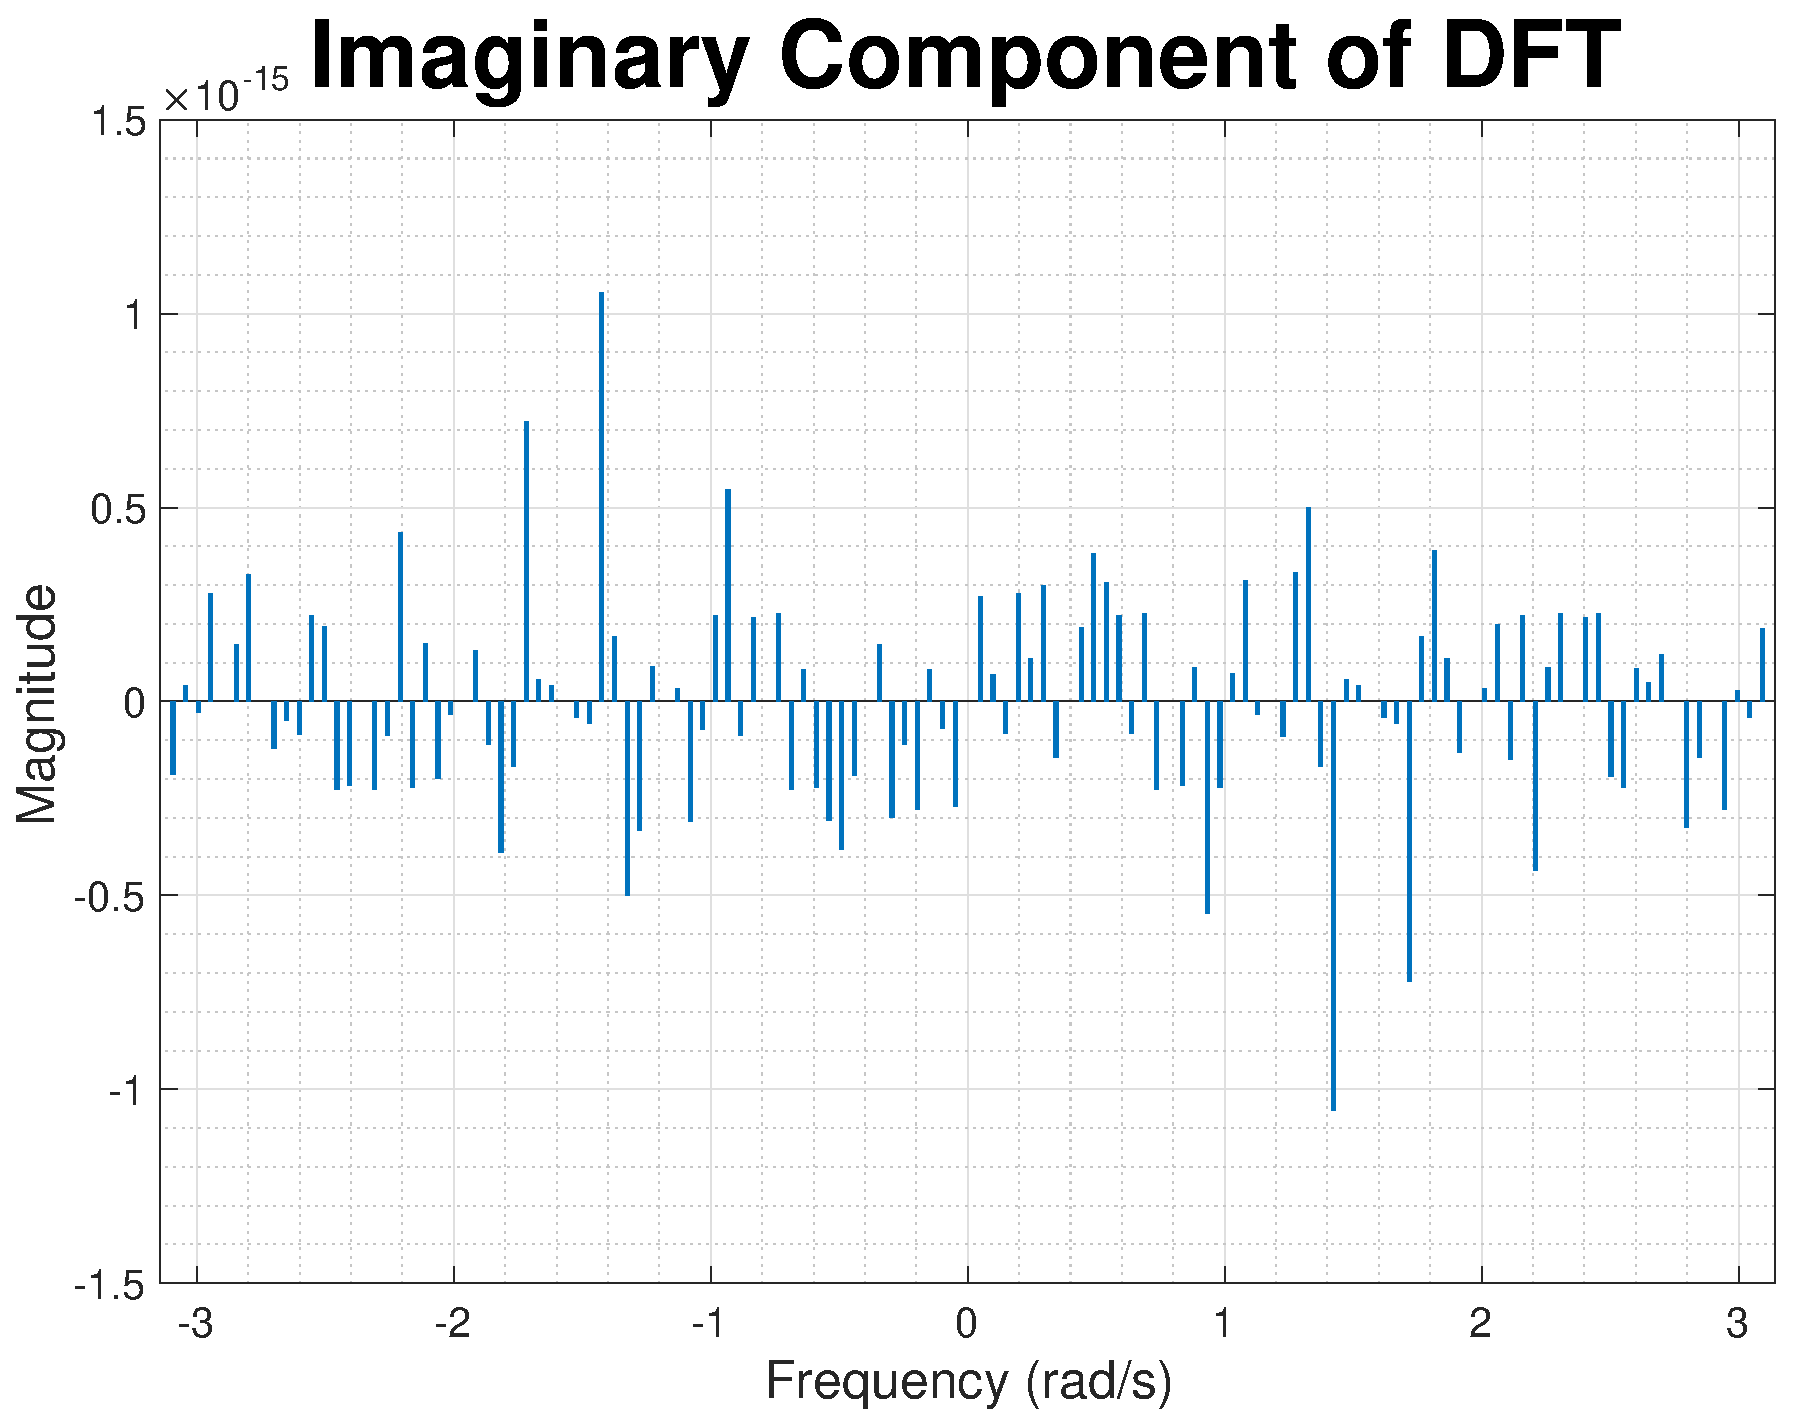
\includegraphics[width=0.32\textwidth]{part1/dft_spectra_acf_x_imag}
\caption{Comparing the magnitudes of the Real and Imaginary Components of $P(\omega_k)$}
\end{figure}


\noindent{}c. The graph below shows that in this case, the real and imaginary components of the DFT are of the same magnitude and thus using the \texttt{real} is not suitable.

\begin{figure}[H]
\centering{}
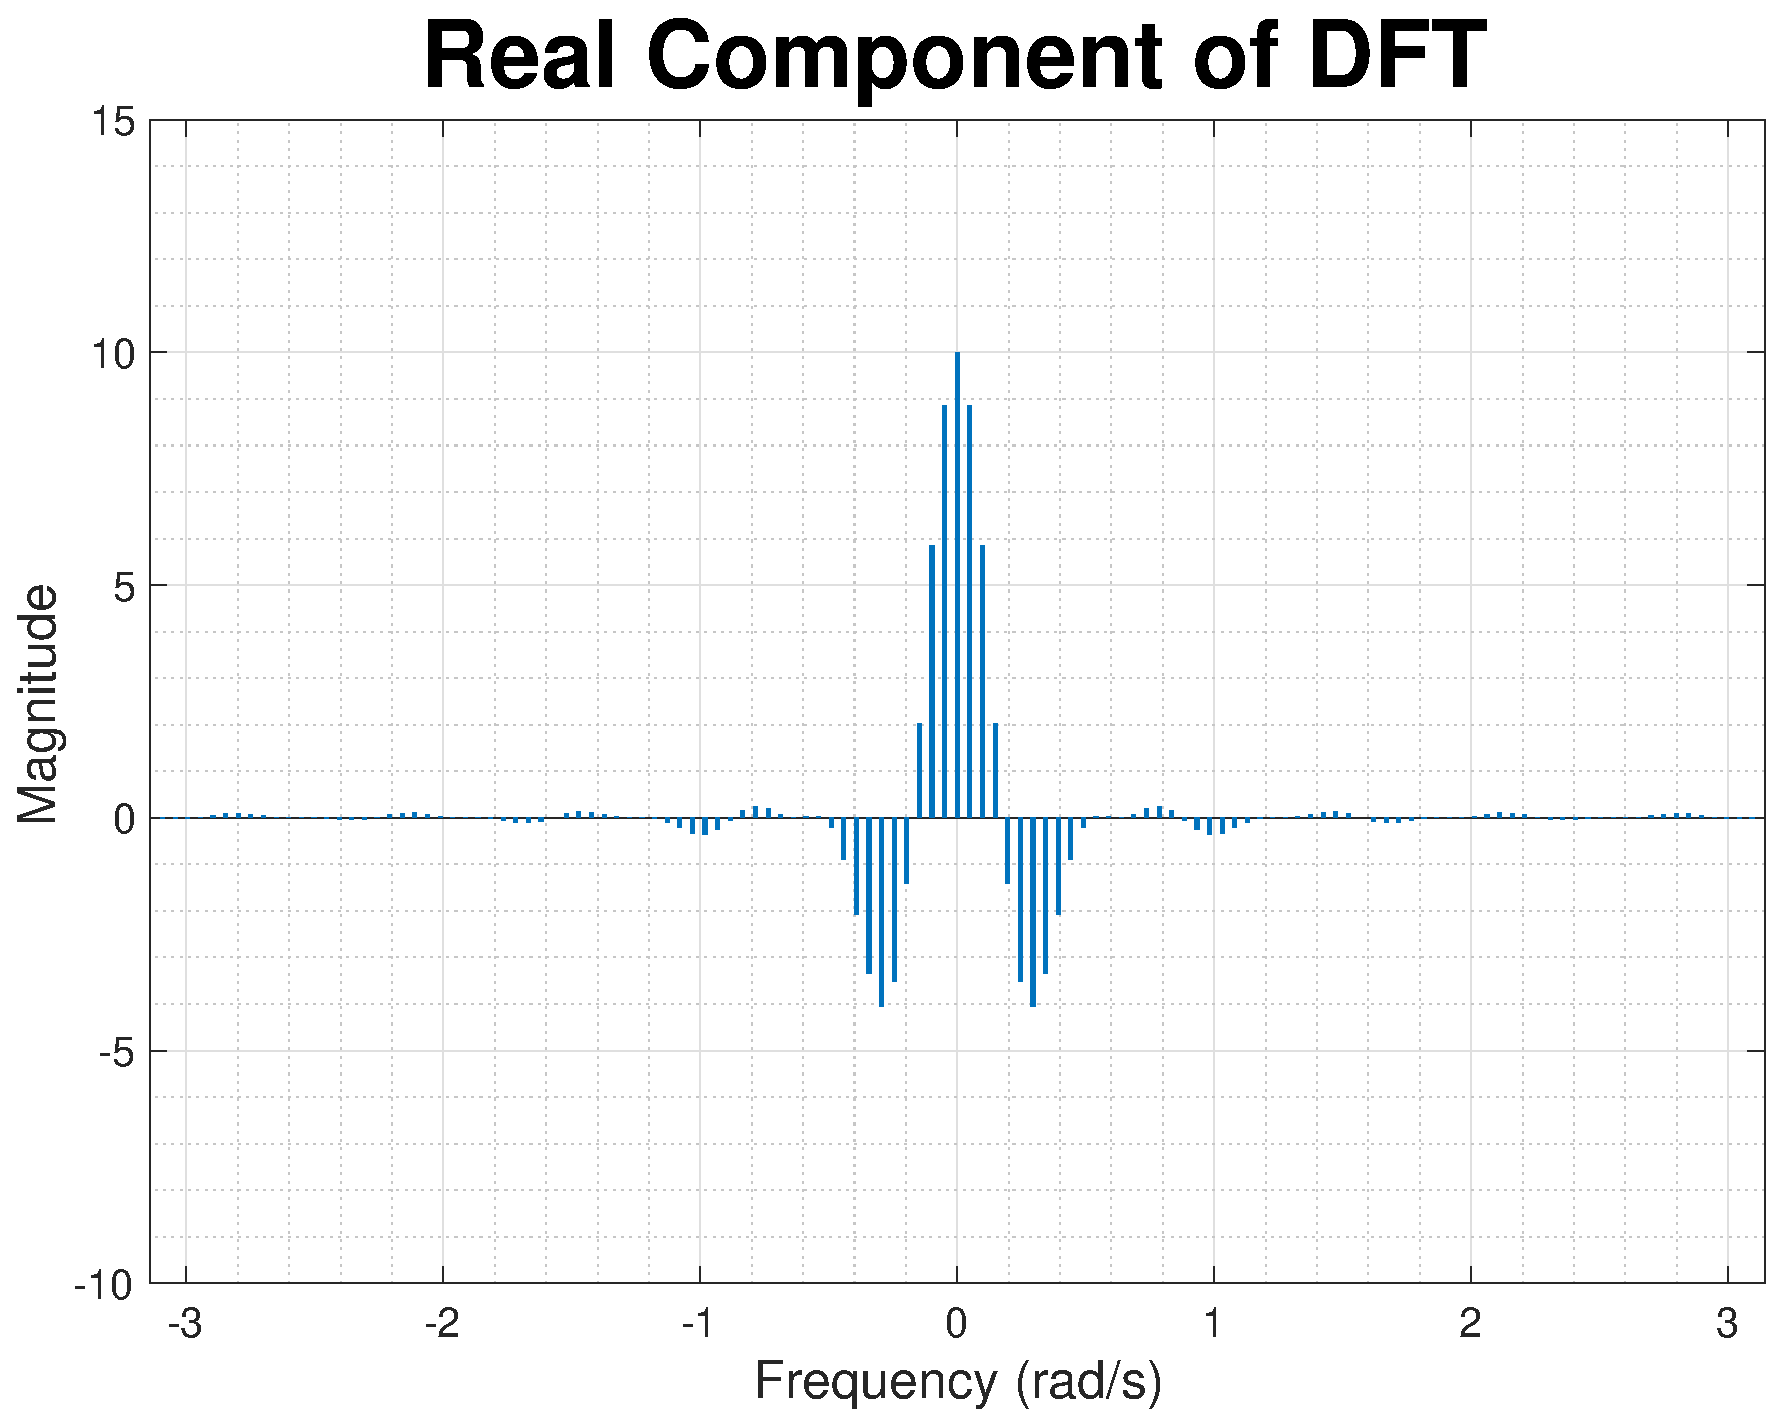
\includegraphics[width=0.32\textwidth]{part1/dft_spectra_acf_z_real}
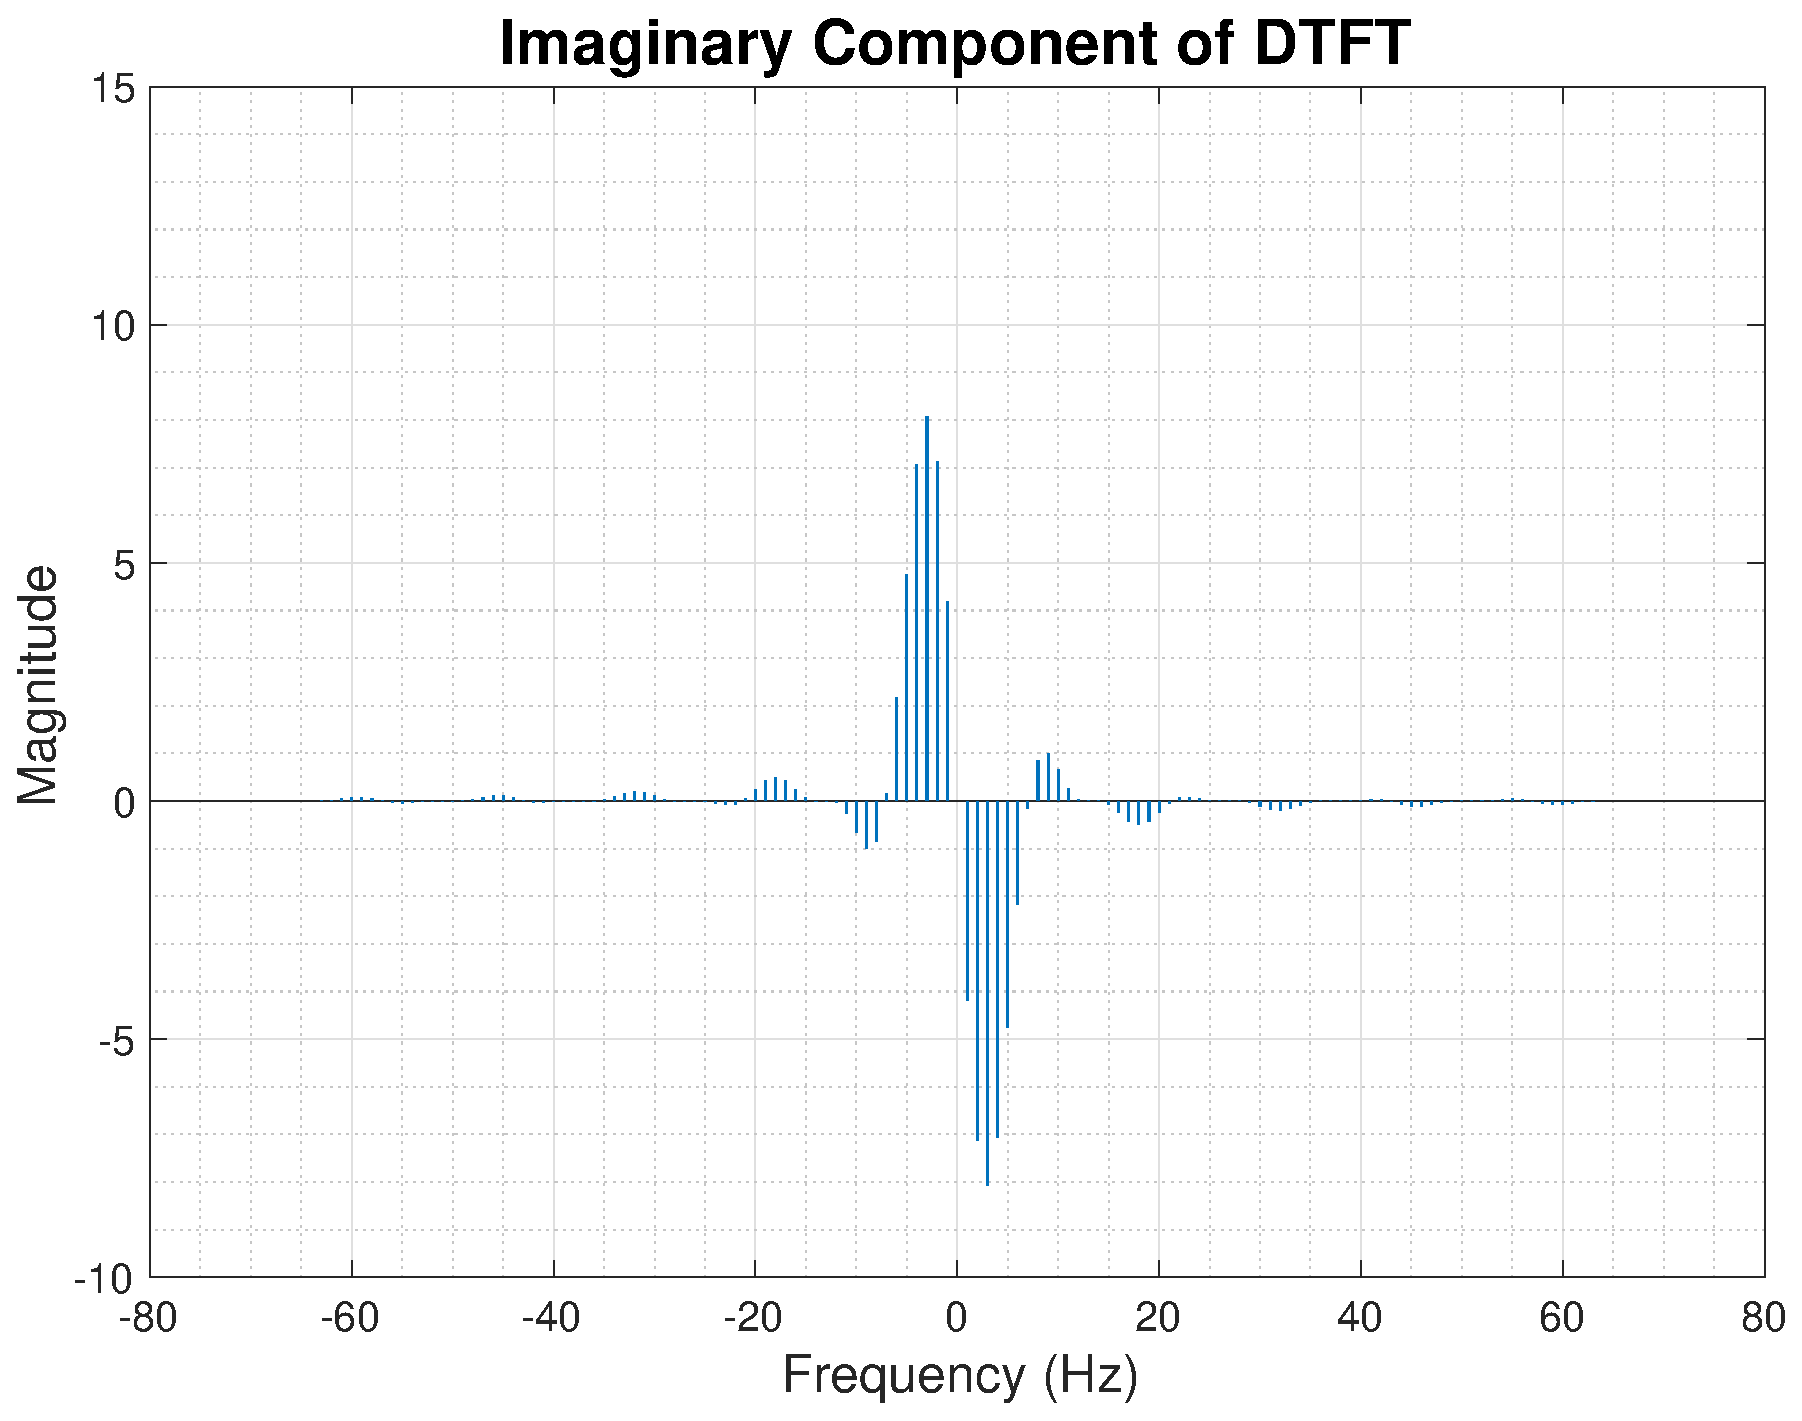
\includegraphics[width=0.32\textwidth]{part1/dft_spectra_acf_z_imag}
\caption{Magnitudes of the Real and Imaginary Components are of the Same Order of Magnitude} 
\end{figure}

\newpage
\noindent{}The correct Power Spectral Density can be obtained using the \texttt{abs} function in a similar fashion to part (a). This is shown in Figure \ref{fig:correct_psd_using_abs}.
\begin{figure}[H]
\centering{}
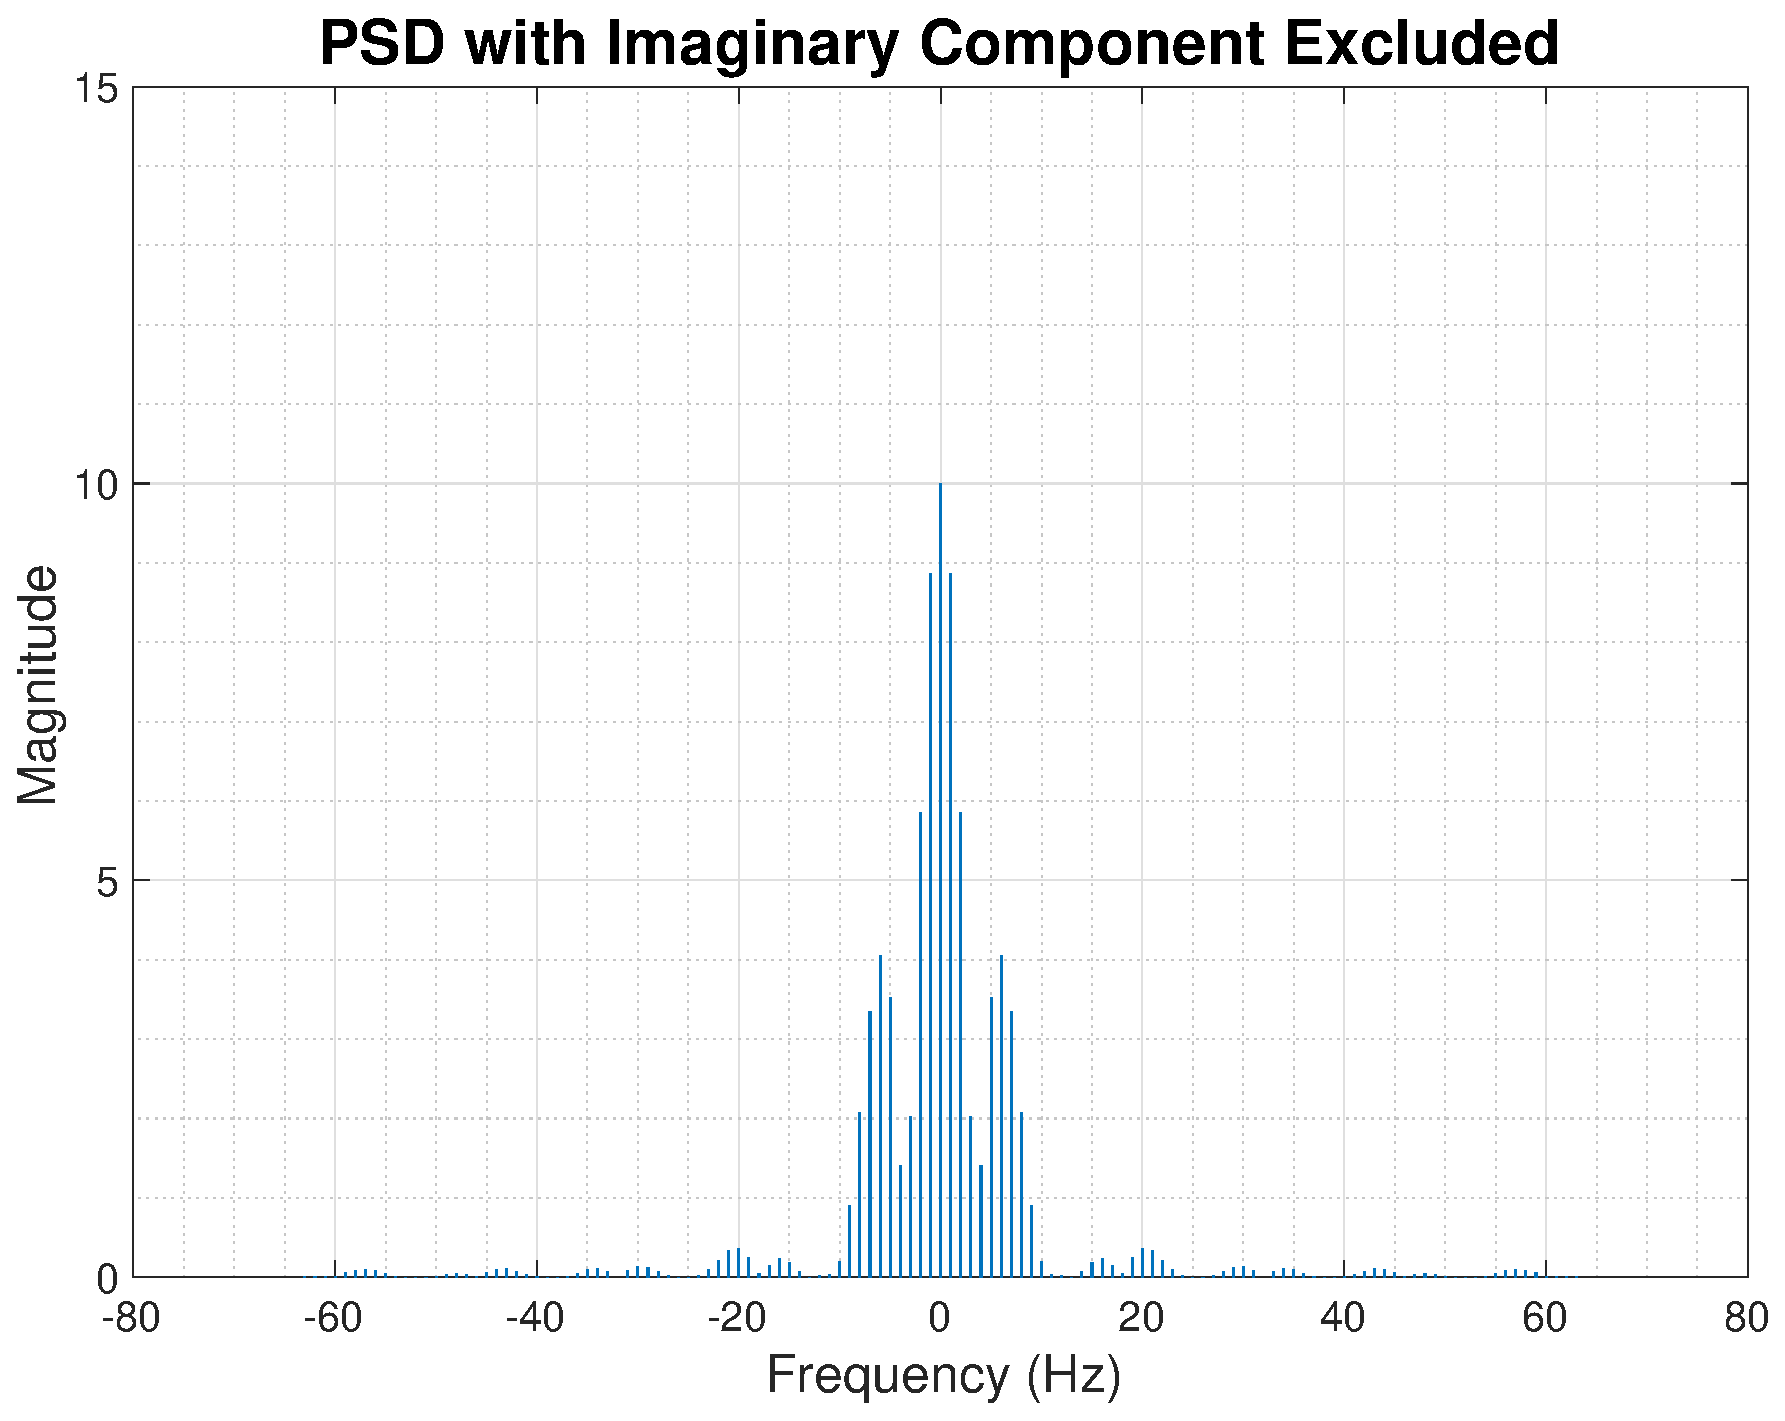
\includegraphics[width=0.32\textwidth]{part1/acf_z_psd_without_imag}
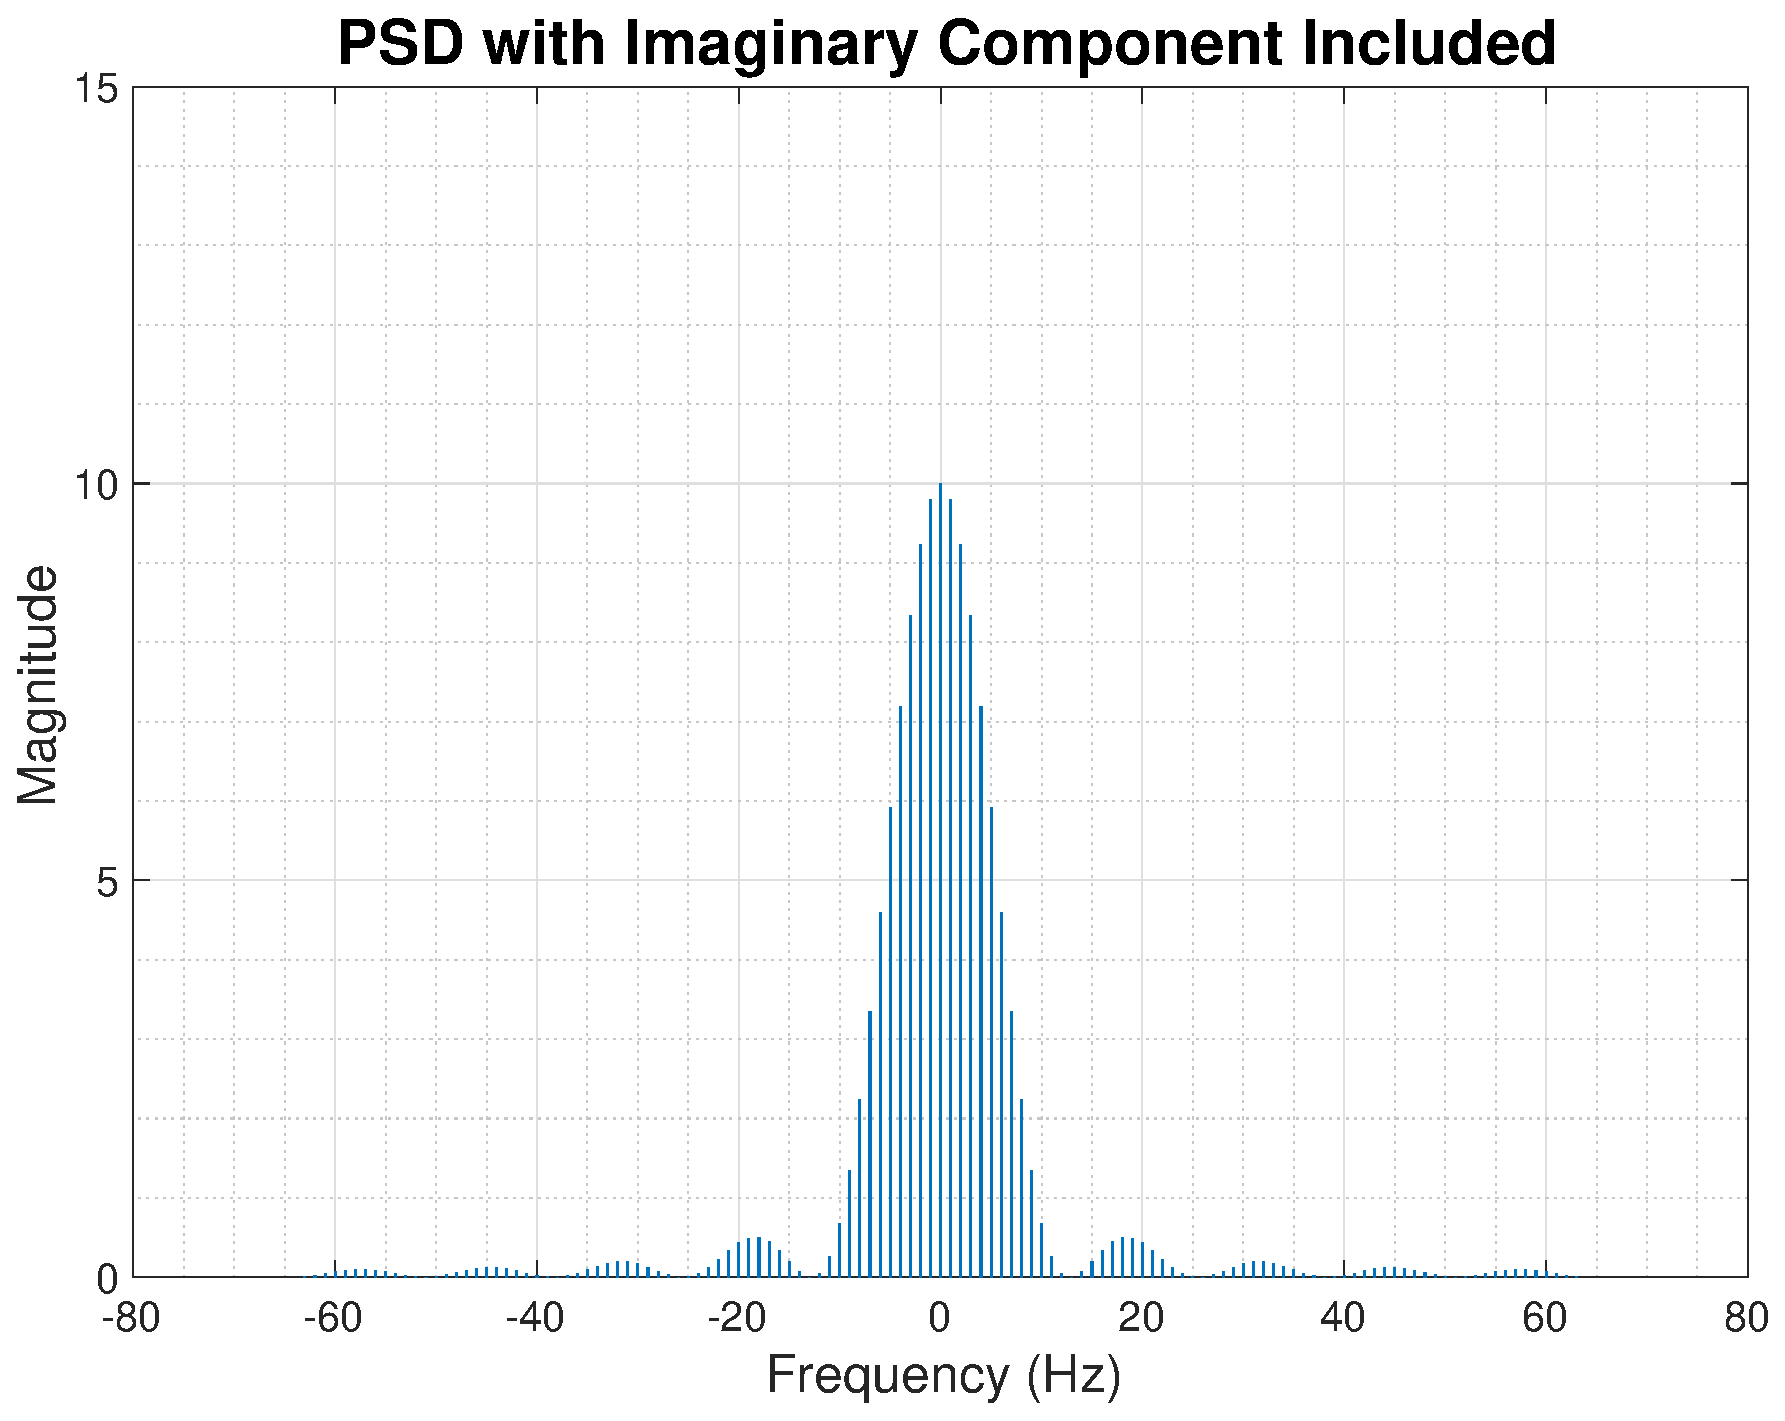
\includegraphics[width=0.32\textwidth]{part1/acf_z_psd_with_imag}
\caption{Erroneous Spectral Values because Imaginary and Real Components are Same Order of Magnitude}
\label{fig:correct_psd_using_abs}
\end{figure}

\noindent{}d. The vectors $\textbf{w}$ and $\textbf{n}$ do indeed depend on if the sequence is odd or even. The formula are described in the table below.

\begin{table}[H]
\tabulinesep=0.9mm
\centering
    \begin{tabu}{|c|c|c|c|c|c|}
        \hline
        \textbf{Sequence Type} & \textbf{Formula for $\textbf{w}$} & \textbf{Formula for $\textbf{n}$} \\
        \hline
        \textbf{Even} & $-\pi:\frac{2\pi}{L}:\pi-\frac{2\pi}{L}$ & $-\frac{L}{2}:1:\frac{L}{2}-1$ \\
        \hline
        \textbf{Odd} & $-\pi+\frac{\pi}{L}:\frac{2\pi}{L-1}:\pi-\frac{\pi}{L}$ & $-\frac{L-1}{2}:1:\frac{L-1}{2}$ \\
        \hline
    \end{tabu}%
  \caption{Formule for vectors $\textbf{w}$ and $\textbf{n}$}
\end{table}%


\subsection{Resolution and Leakage of Periodogram-based Methods}


\noindent{}Figure \ref{fig:bartlett_window_log_linear} shows the magnitude spectrum of the Bartlett Window for $N=128$ and $N=512$ on both linear and logarithmic scales. The red line is graphed to show the 3 dB frequency of each window. 

\begin{figure}[H]
\centering{}
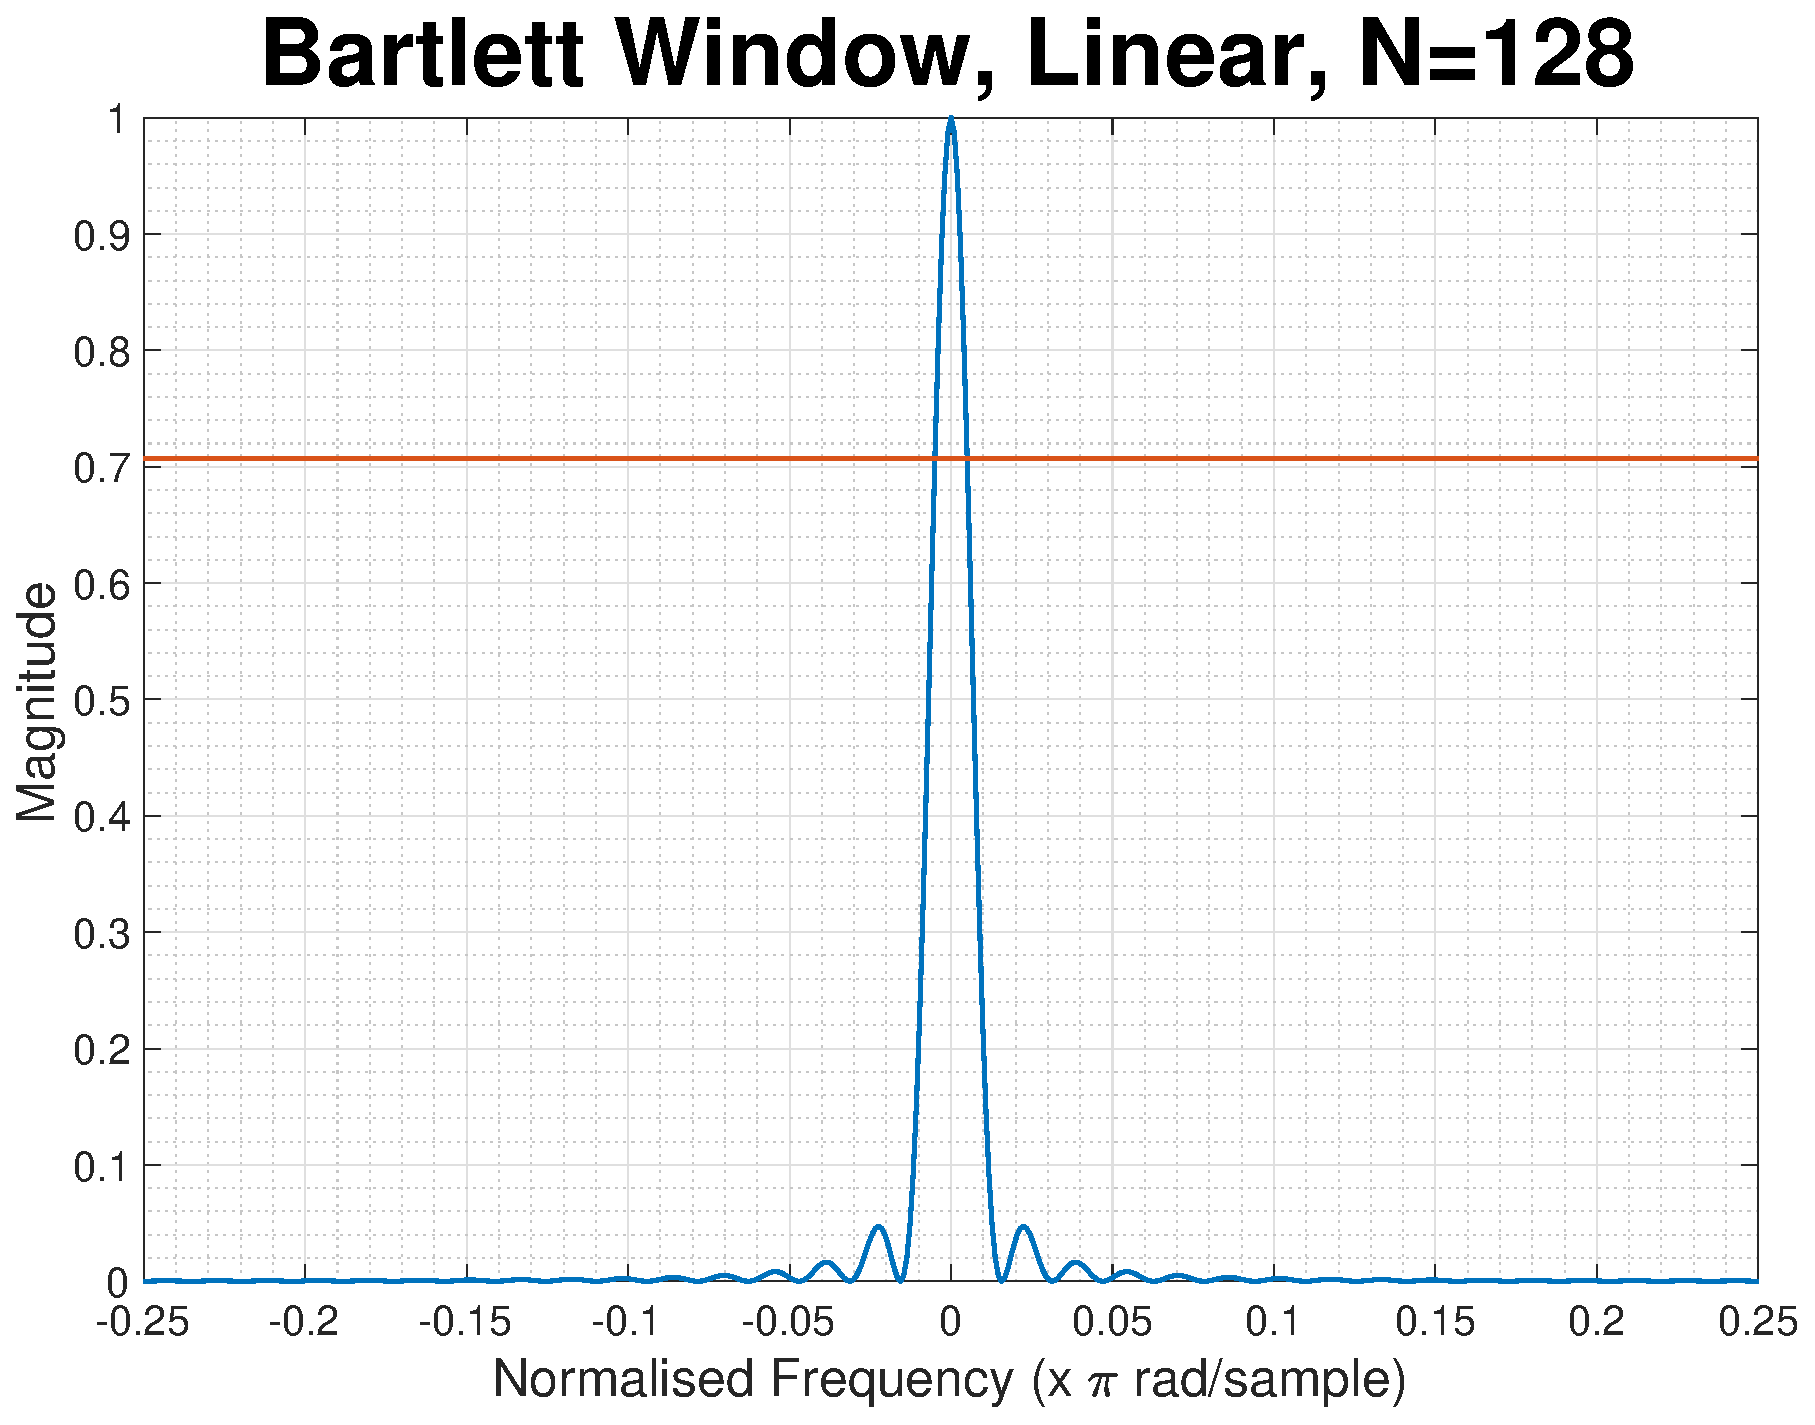
\includegraphics[width=0.32\textwidth]{part1/bartlett_window_N_128_linear}
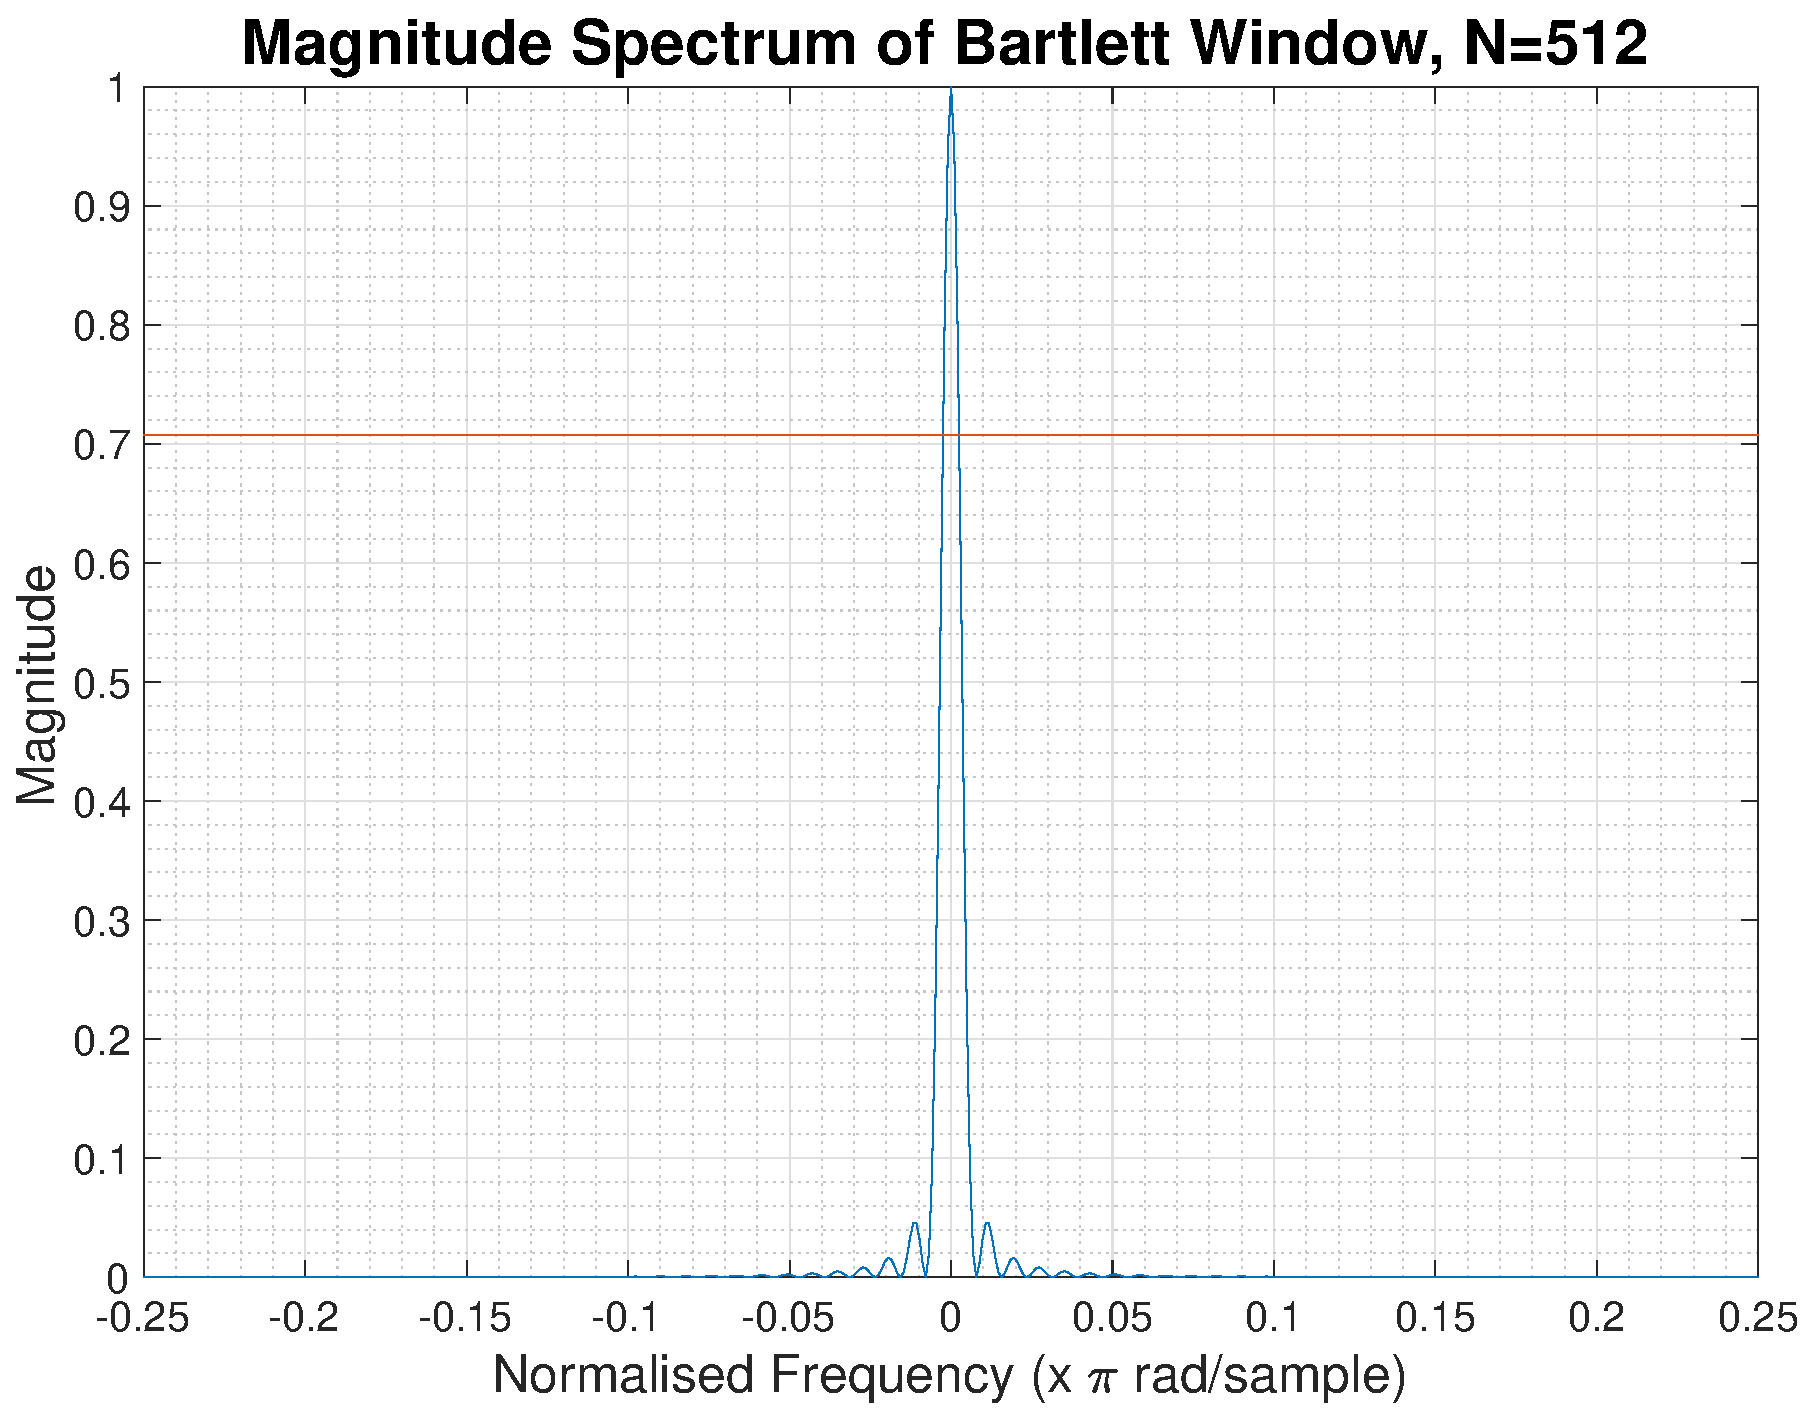
\includegraphics[width=0.32\textwidth]{part1/bartlett_window_N_512_linear} \\
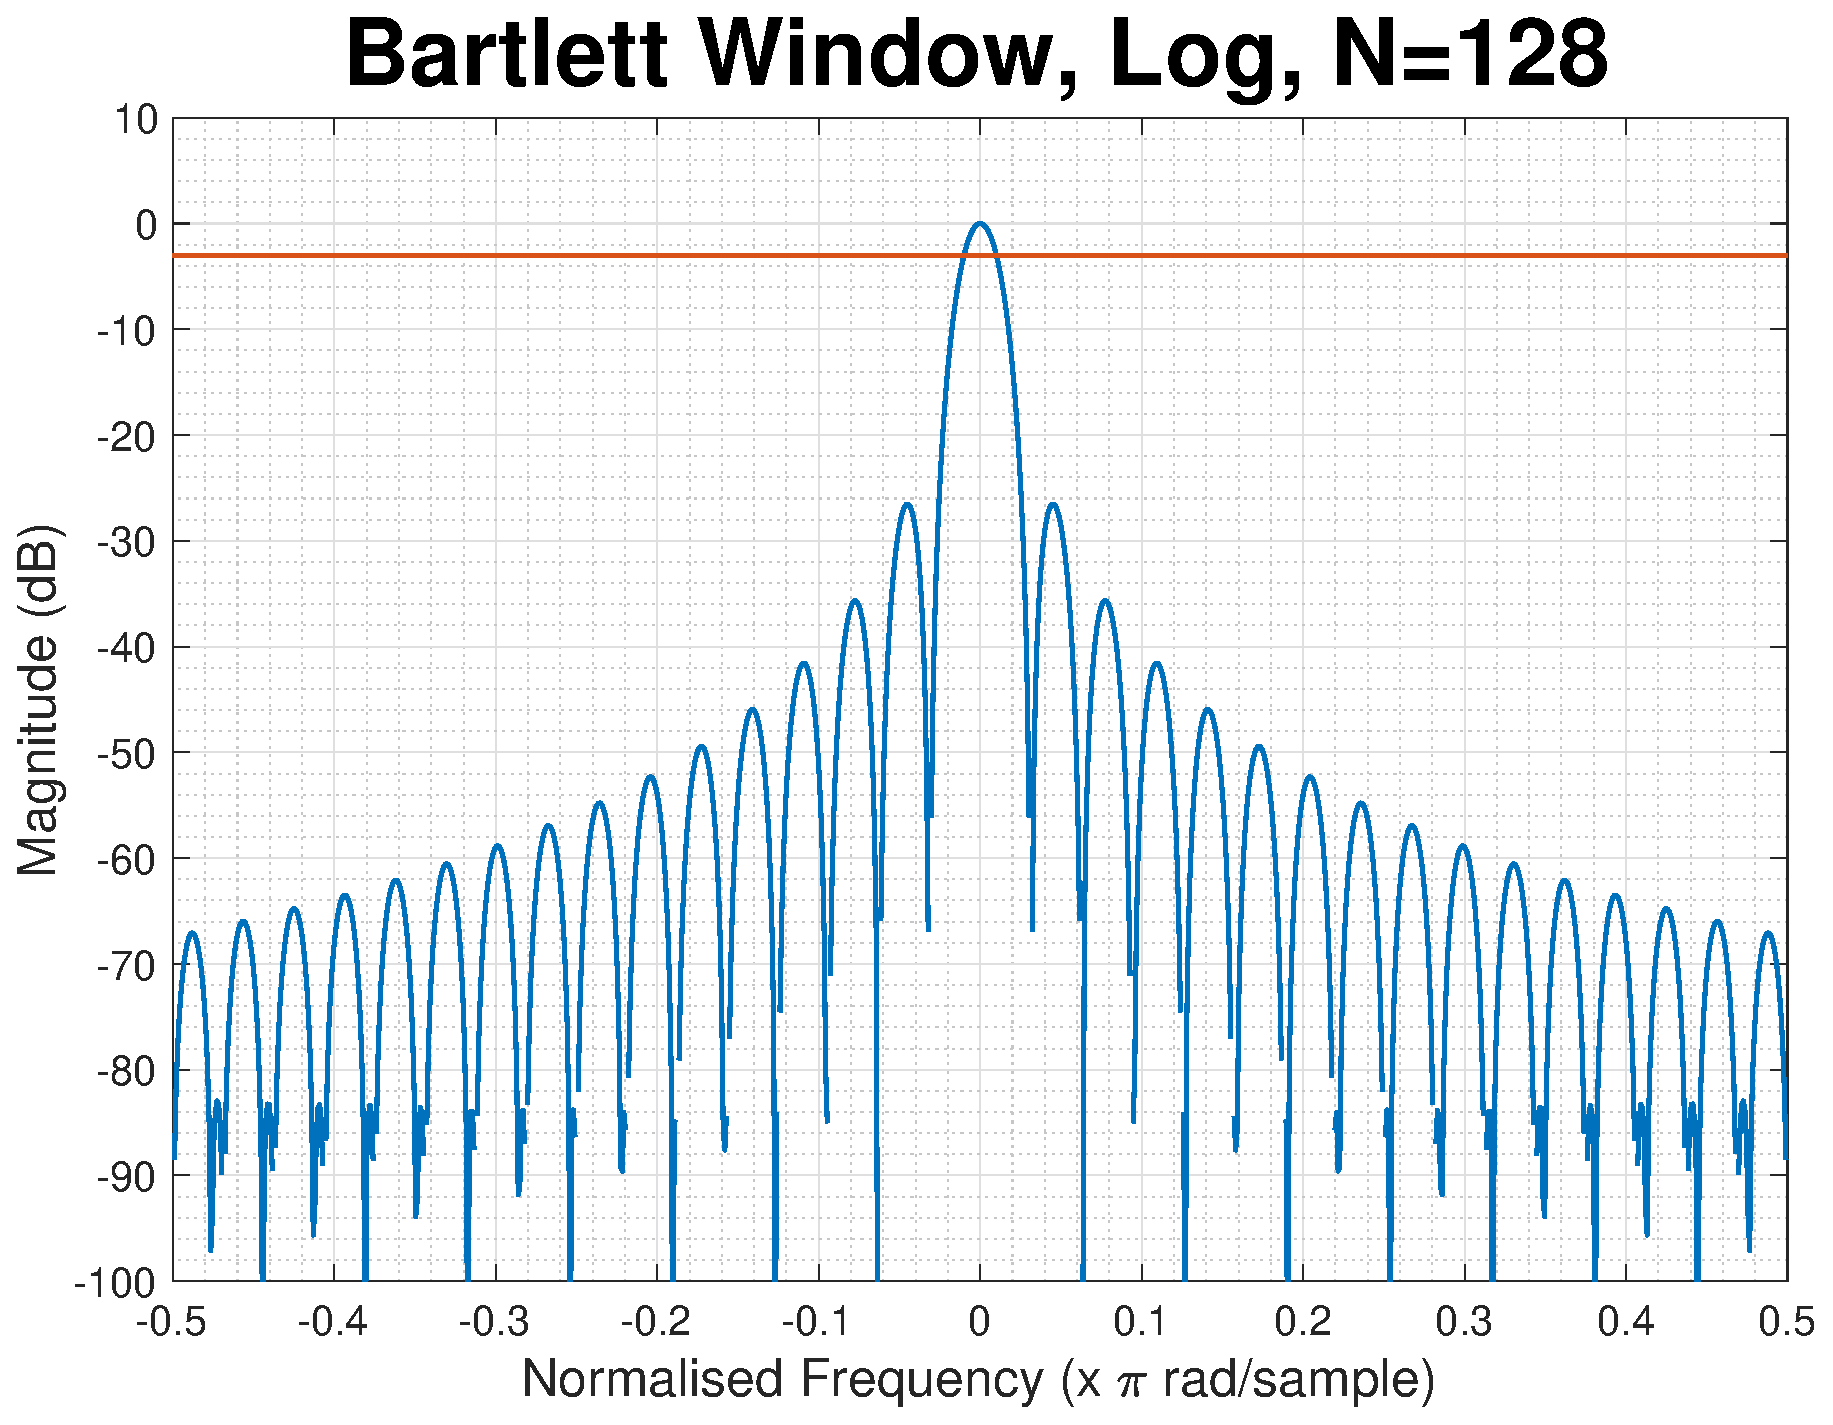
\includegraphics[width=0.32\textwidth]{part1/bartlett_window_N_128_dB}
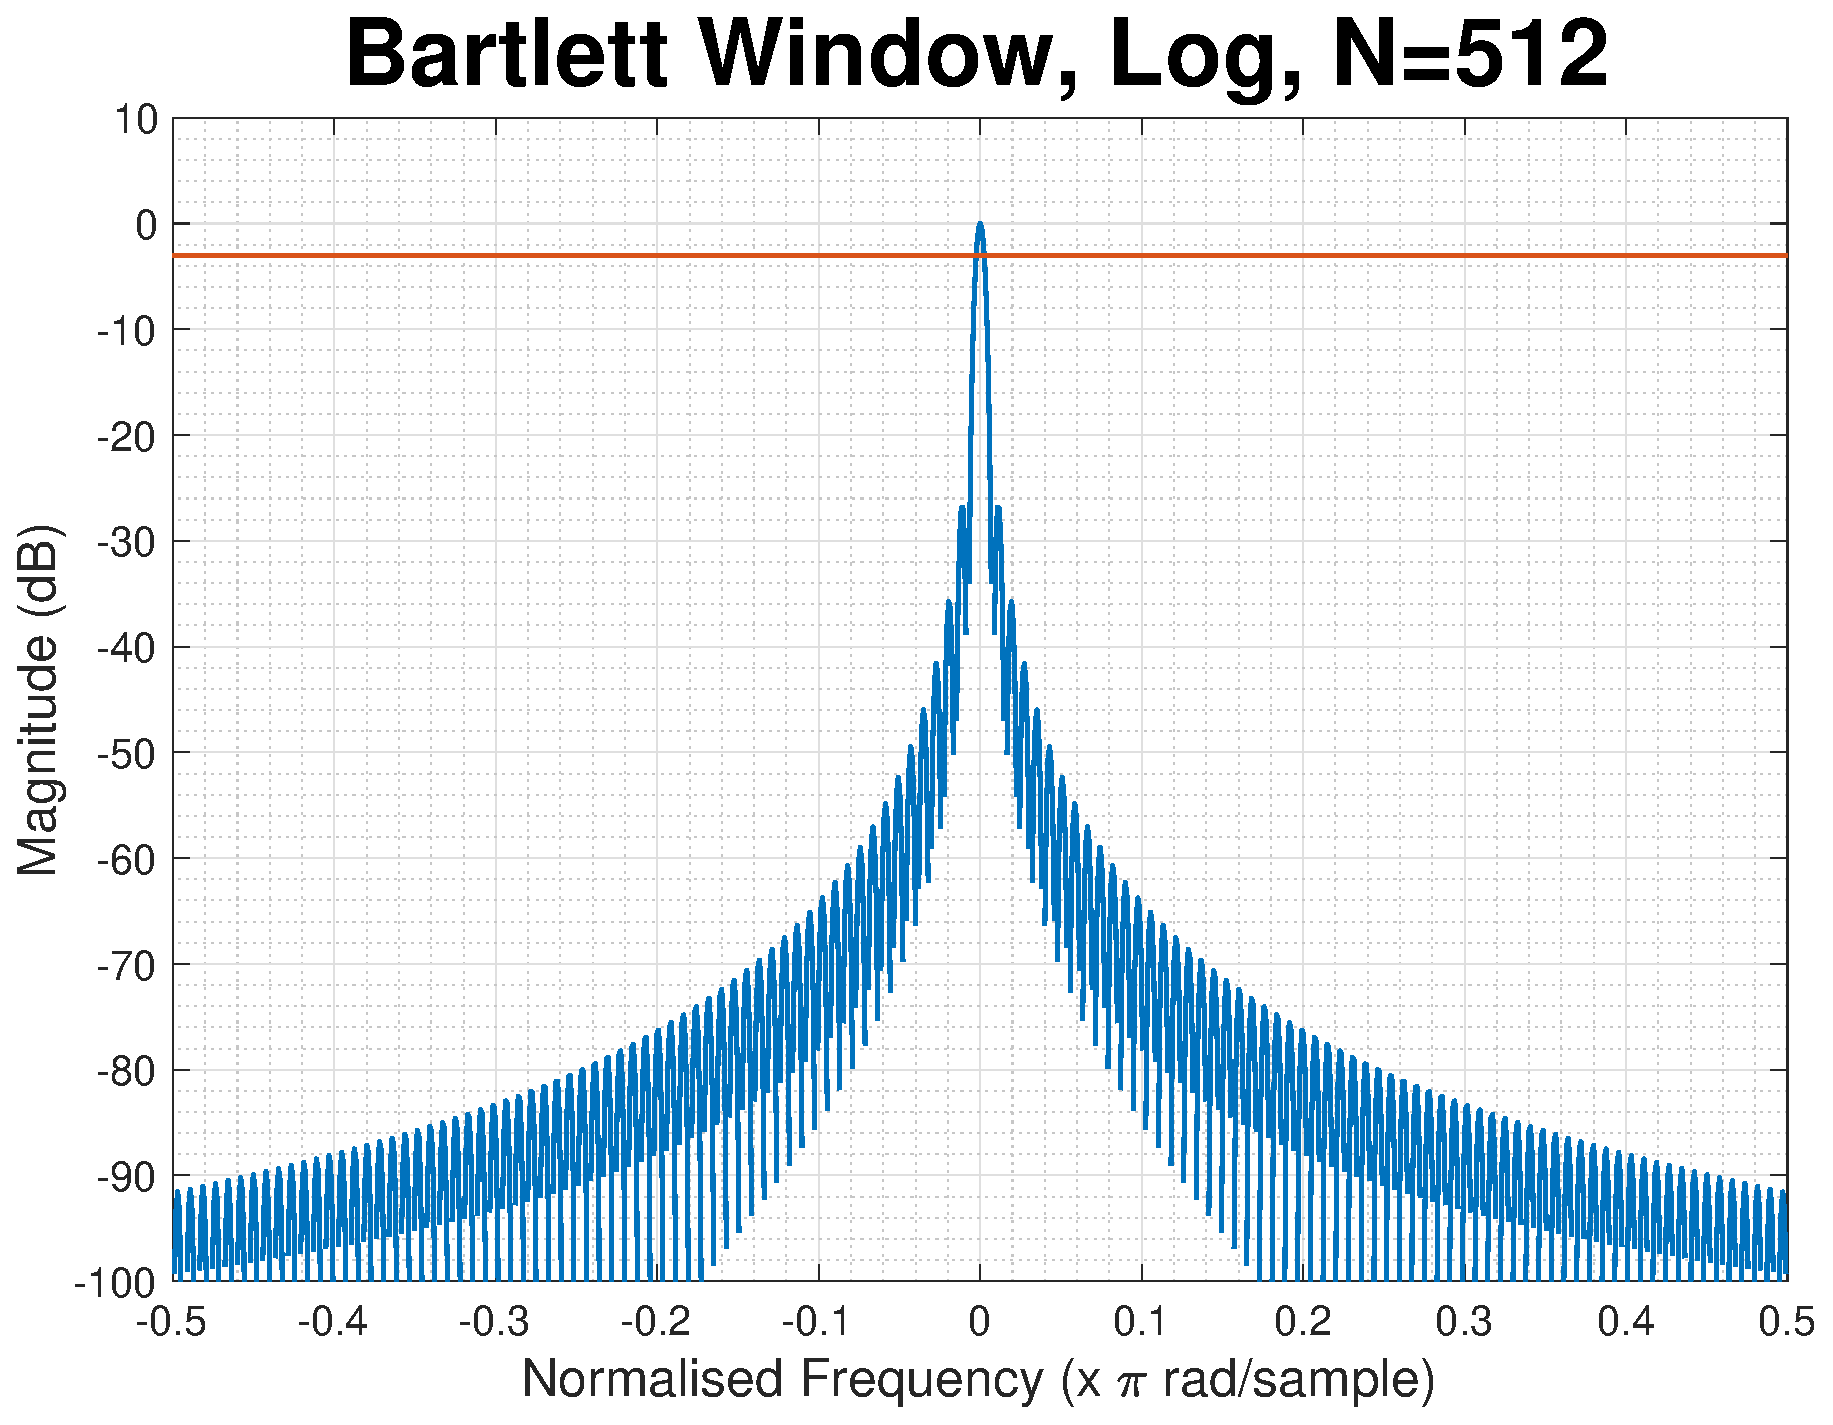
\includegraphics[width=0.32\textwidth]{part1/bartlett_window_N_512_dB}
\caption{Bartlett Window with Linear and Log Scales for $N=128$ and $N=512$}
\label{fig:bartlett_window_log_linear}
\end{figure}

\noindent{}To find the relationship between the width of the mainlobe and the length of the window, the 3 dB frequency is evaluated for a range of window lengths\footnote{The intersection points were found using the function \texttt{InterX} found on matlab file exchange.}. The figure below shows the relationship between the empirical 3 dB width of the main lobe of the Bartlett Window, $\omega_{c}$, and both $N$ and $\frac{1}{N}$. 

\begin{figure}[H]
\centering{}
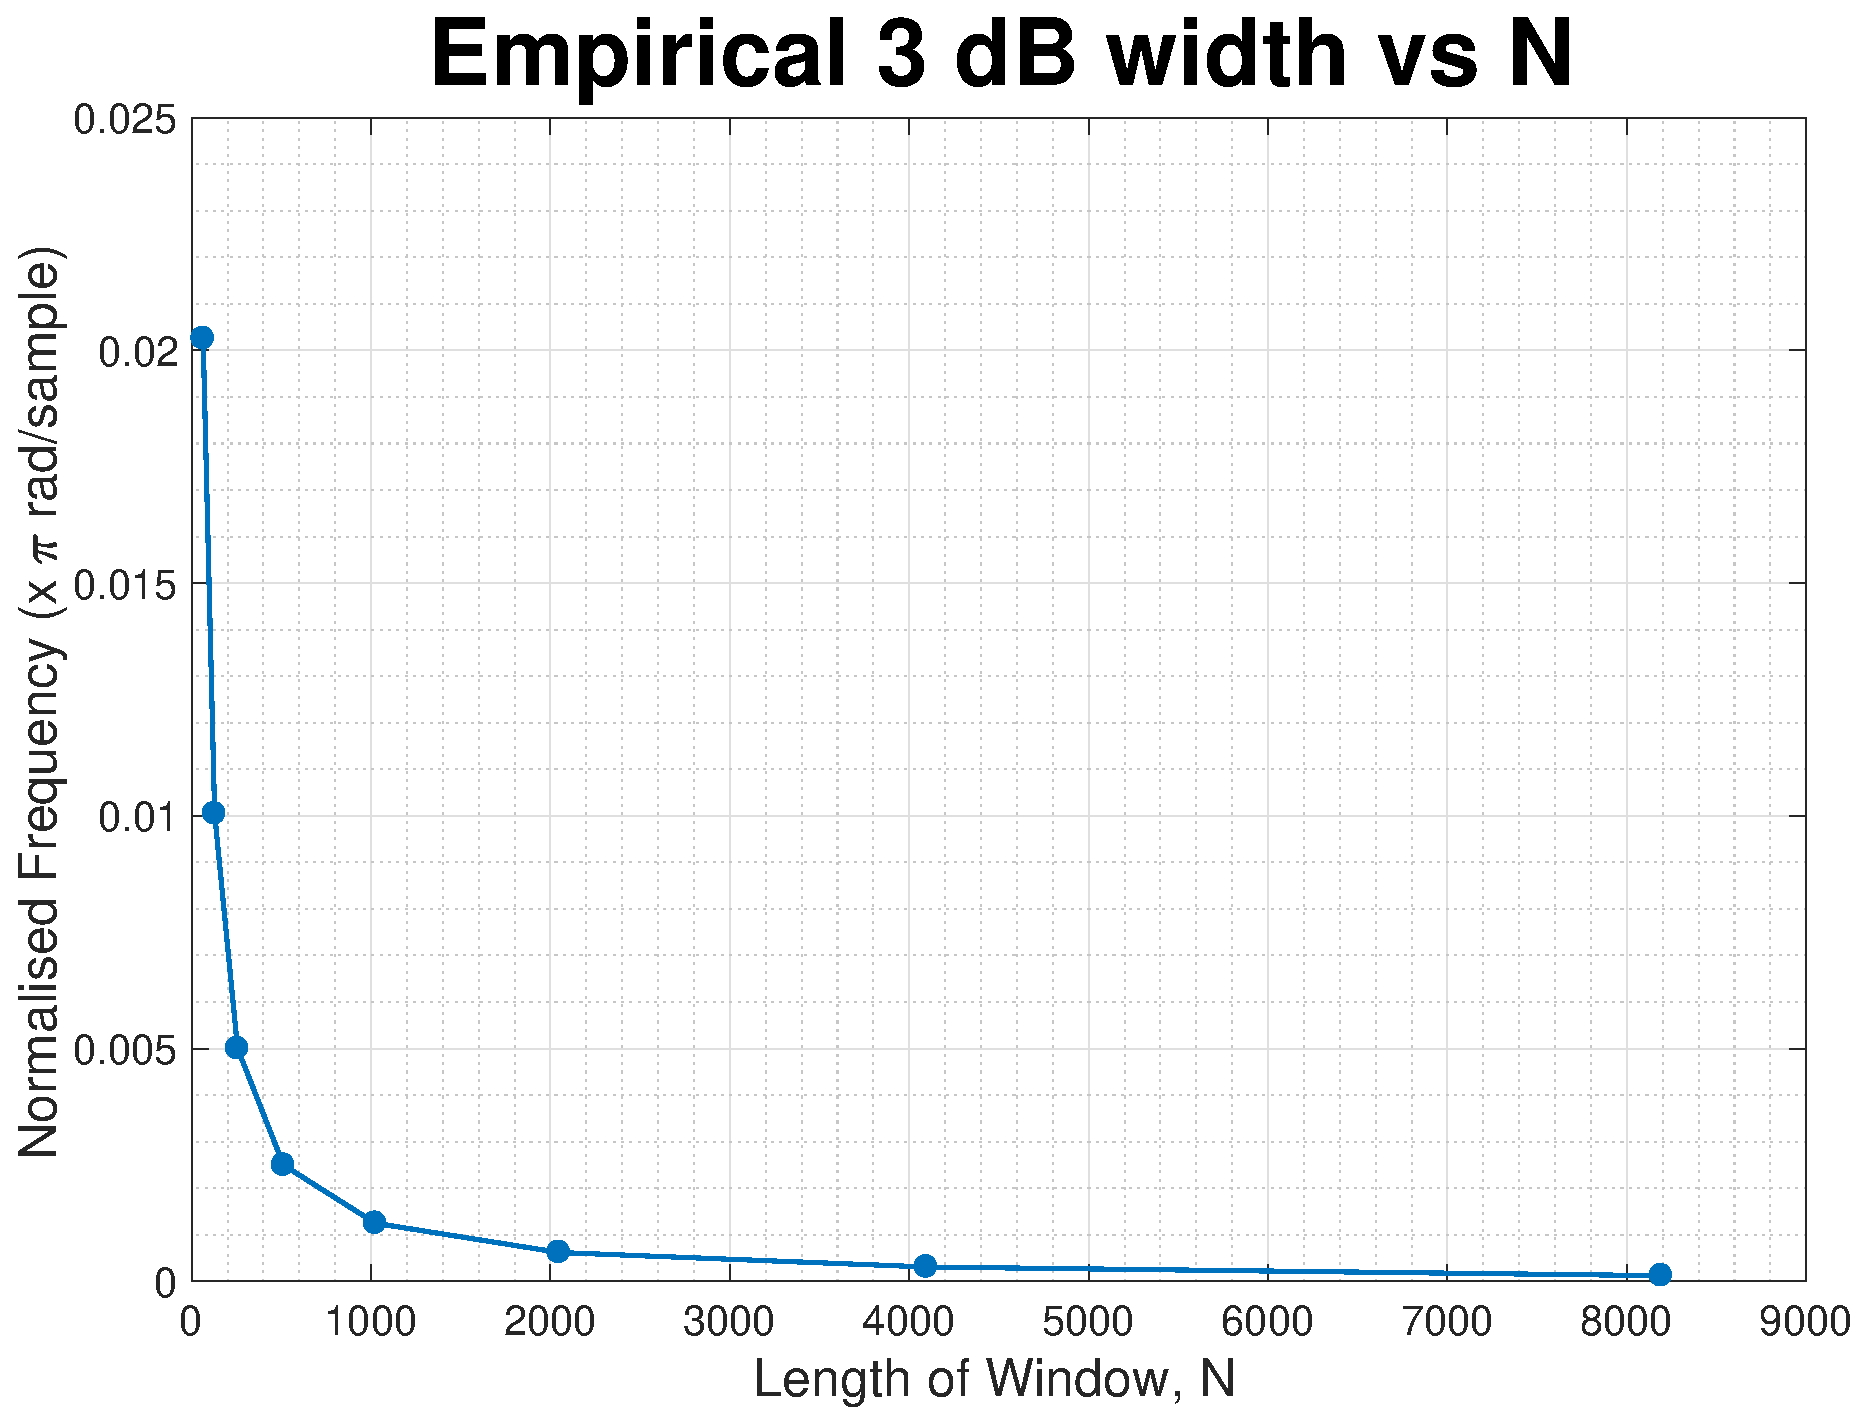
\includegraphics[width=0.32\textwidth]{part1/bartlett_empirical_vs_N}
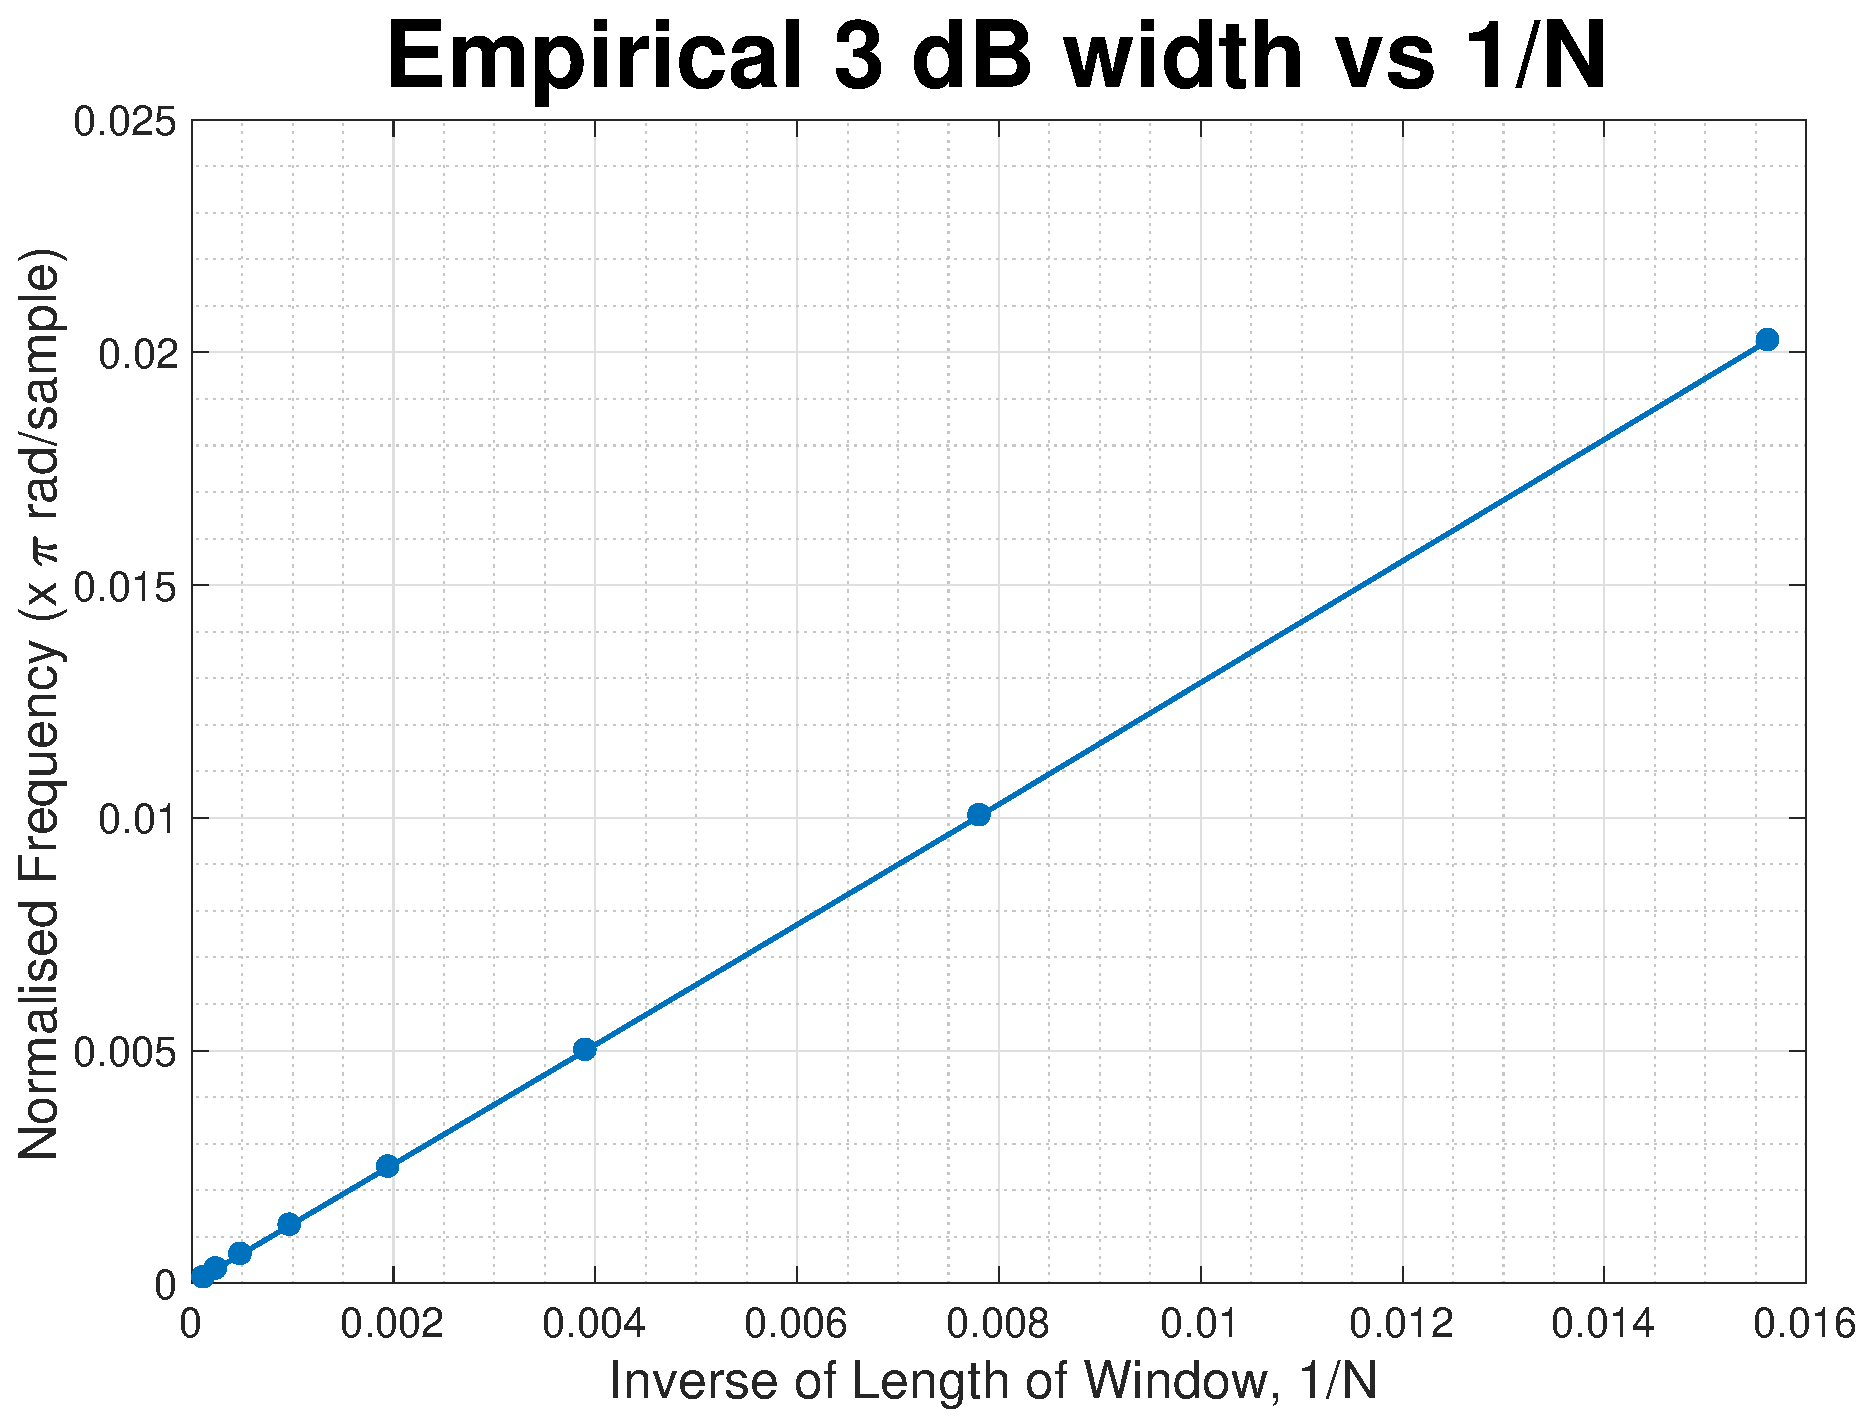
\includegraphics[width=0.32\textwidth]{part1/bartlett_empirical_vs_1_over_N}
\caption{Empirical Relationship between 3 dB width of Mainlobe for Bartlett Window and Window Length}
\end{figure}

\noindent{}In matlab, a linear relationship between frequency and $1/N$ is obtained using \texttt{pinv}. The linear relationship is:

\begin{align*}
\omega_{c}=\frac{1.2965(2\pi)}{N}
\end{align*}


\noindent{}The figure below shows the independence of the sidelobe peak to window length. The sidelobe peak is at a constant value of -26.5 dB relative to the height of the mainlobe.

\begin{figure}[H]
\centering{}
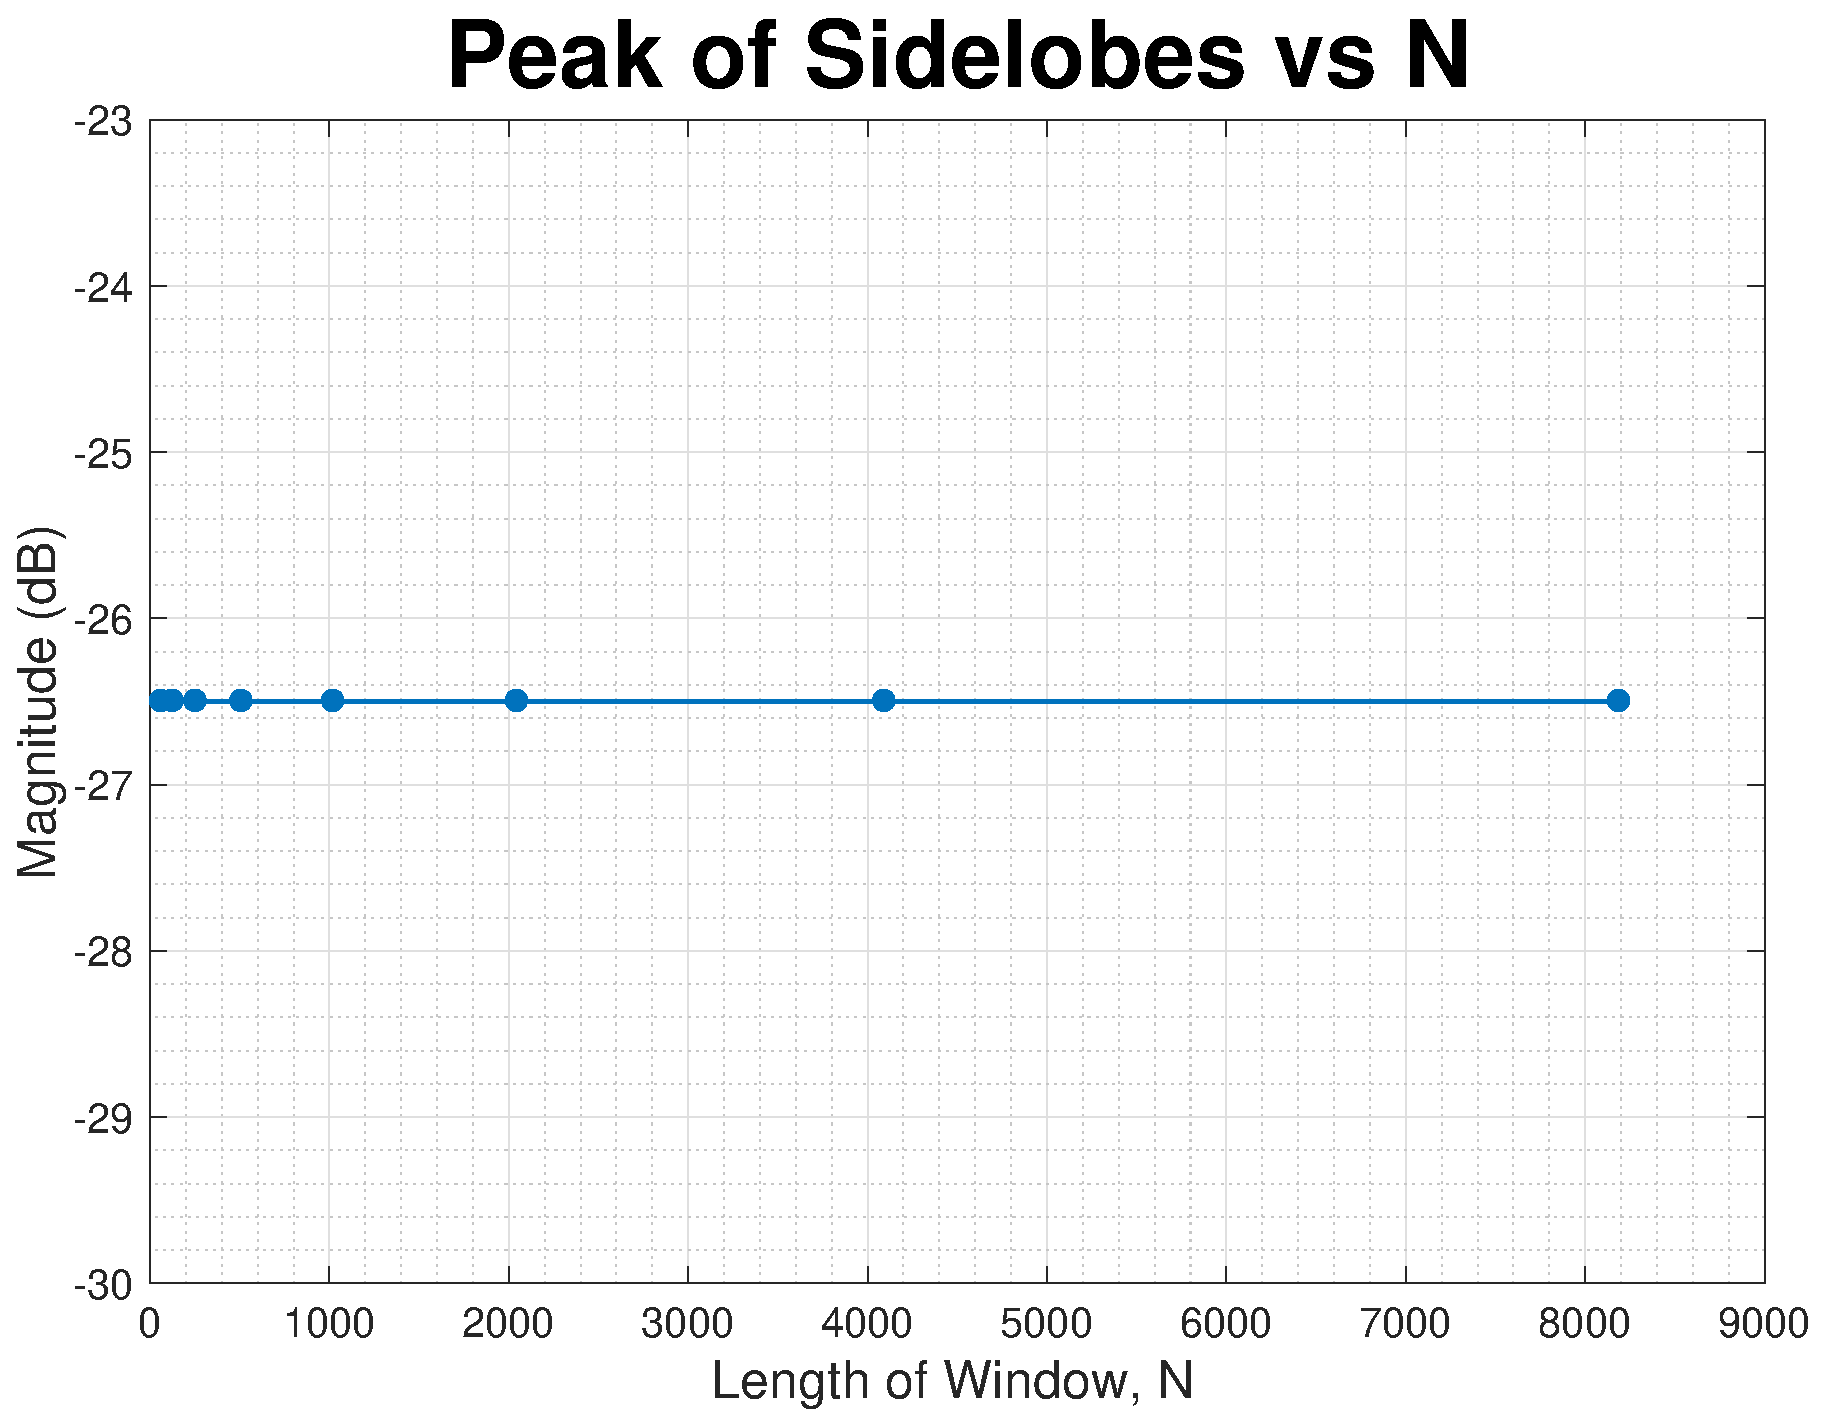
\includegraphics[width=0.32\textwidth]{part1/bartlett_empirical_side_lobe}
\caption{Empirical Relationship between Sidelobe Peak for Bartlett Window and Window Length}
\end{figure}

\noindent{}b. The signal $x(n)$ has been very carefully designed to study the frequency resolutions of different windows. This is because the frequency of one sine wave differs from the frequency of the other by a factor of $\frac{\alpha 2\pi}{N}$; The resolution of a spectral estimation method has the following general form described in (\ref{eq:periodogram_res_general_form}). Thus, the signal $x(n)$ can be used to understand the scaling factor.

\begin{align}
\text{Res}\Bigg[\hat{P}_{per}\bigg(e^{j\omega}\bigg)\Bigg] = c\frac{2\pi}{N} \label{eq:periodogram_res_general_form}
\end{align}

\noindent{}The following graphs show the periodograms for $\alpha \in \{1, 0.65, 0.60\}$. It is clear that for values of $\alpha \leq 0.60$, the two peaks are not distinguishable. This value of alpha is significantly smaller than the value quoted in the lecture notes and in \cite{hayes2009statistical}. The value quoted in both pieces of literature take into account that the periodogram has some noise however we have removed noise and thus achieve greater resolution. 

\begin{figure}[H]
\centering{}
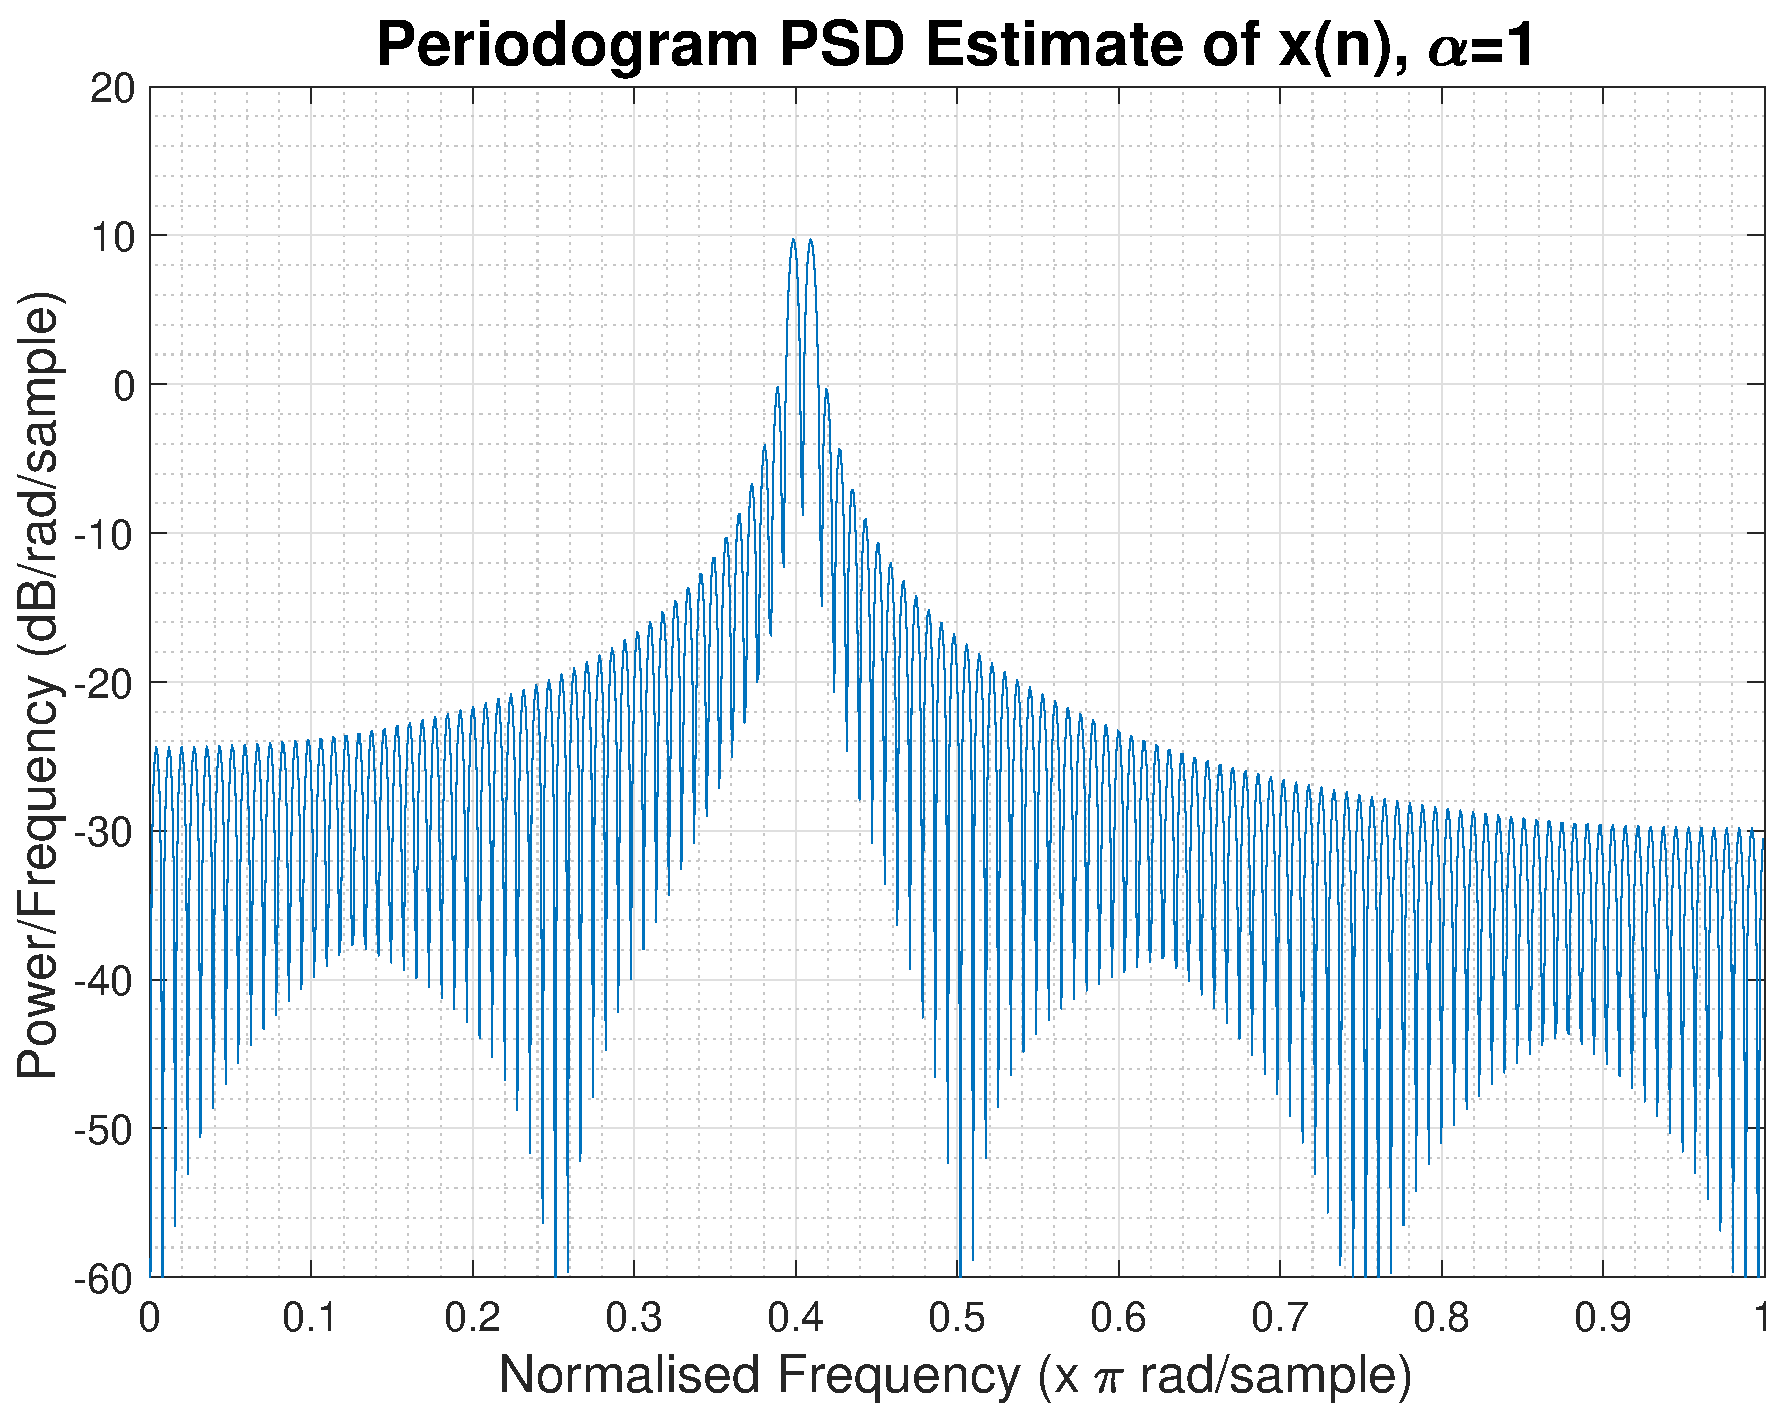
\includegraphics[width=0.32\textwidth]{part1/periodogram_xn_alpha_1}
\includegraphics[width=0.32\textwidth]{part1/periodogram_xn_alpha_point_64}
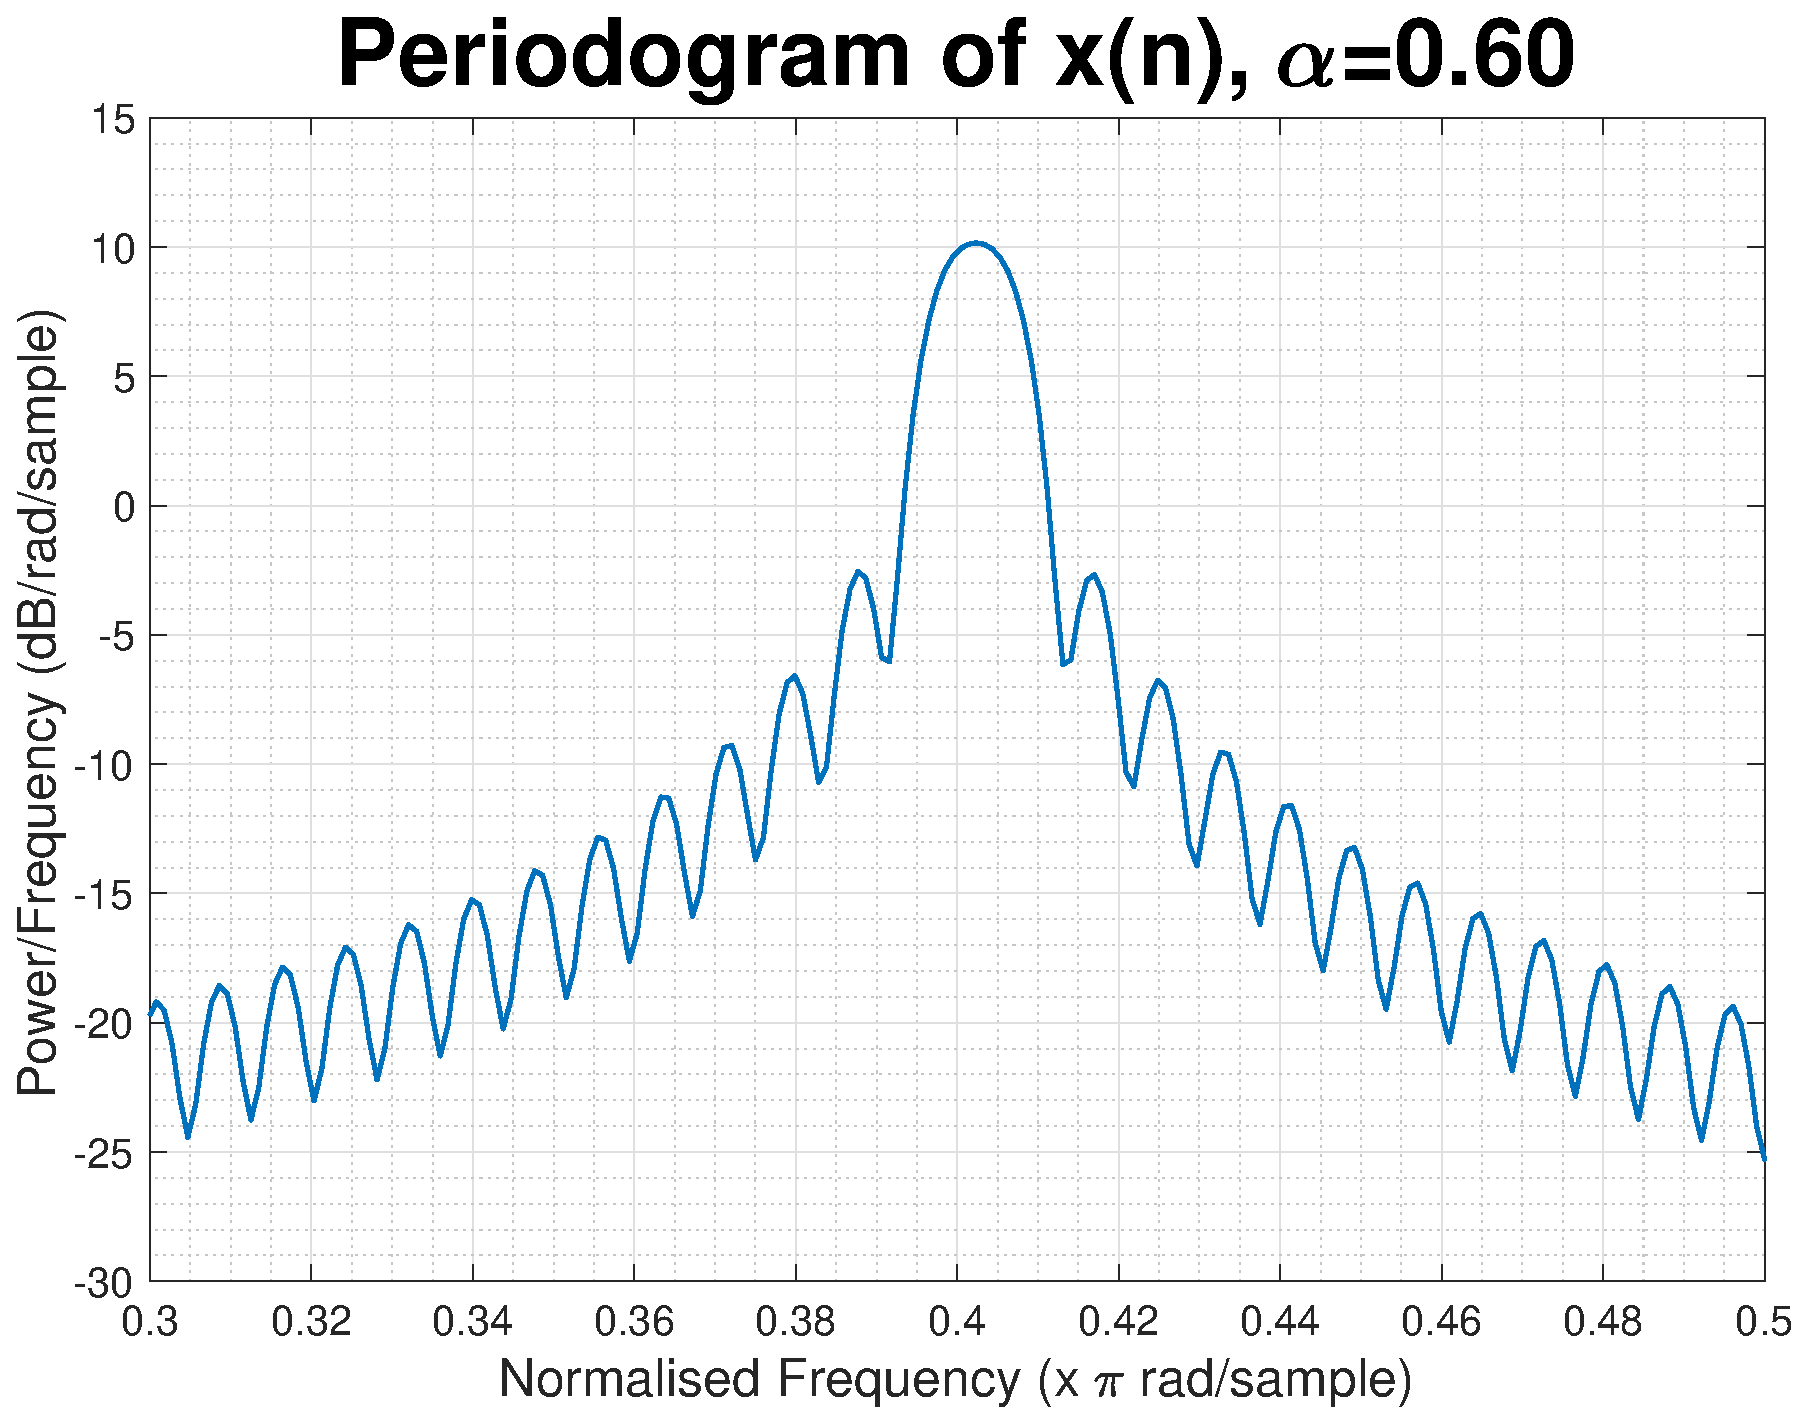
\includegraphics[width=0.32\textwidth]{part1/periodogram_xn_alpha_point_63}
\caption{Periodogram of Signal $x(n)$ for Different Values of $\alpha$}
\end{figure}

\noindent{}c. The hamming window has a wider mainlobe than the rectangular window. As such, the window smears the spectrum to a greater degree and thus the two frequencies are indistinguishable beyond $\alpha=0.70$. Although hamming window has a wider mainlobe, its sidelobes are much lower and this is evident in the figure below. 

\begin{figure}[H]
\centering{}
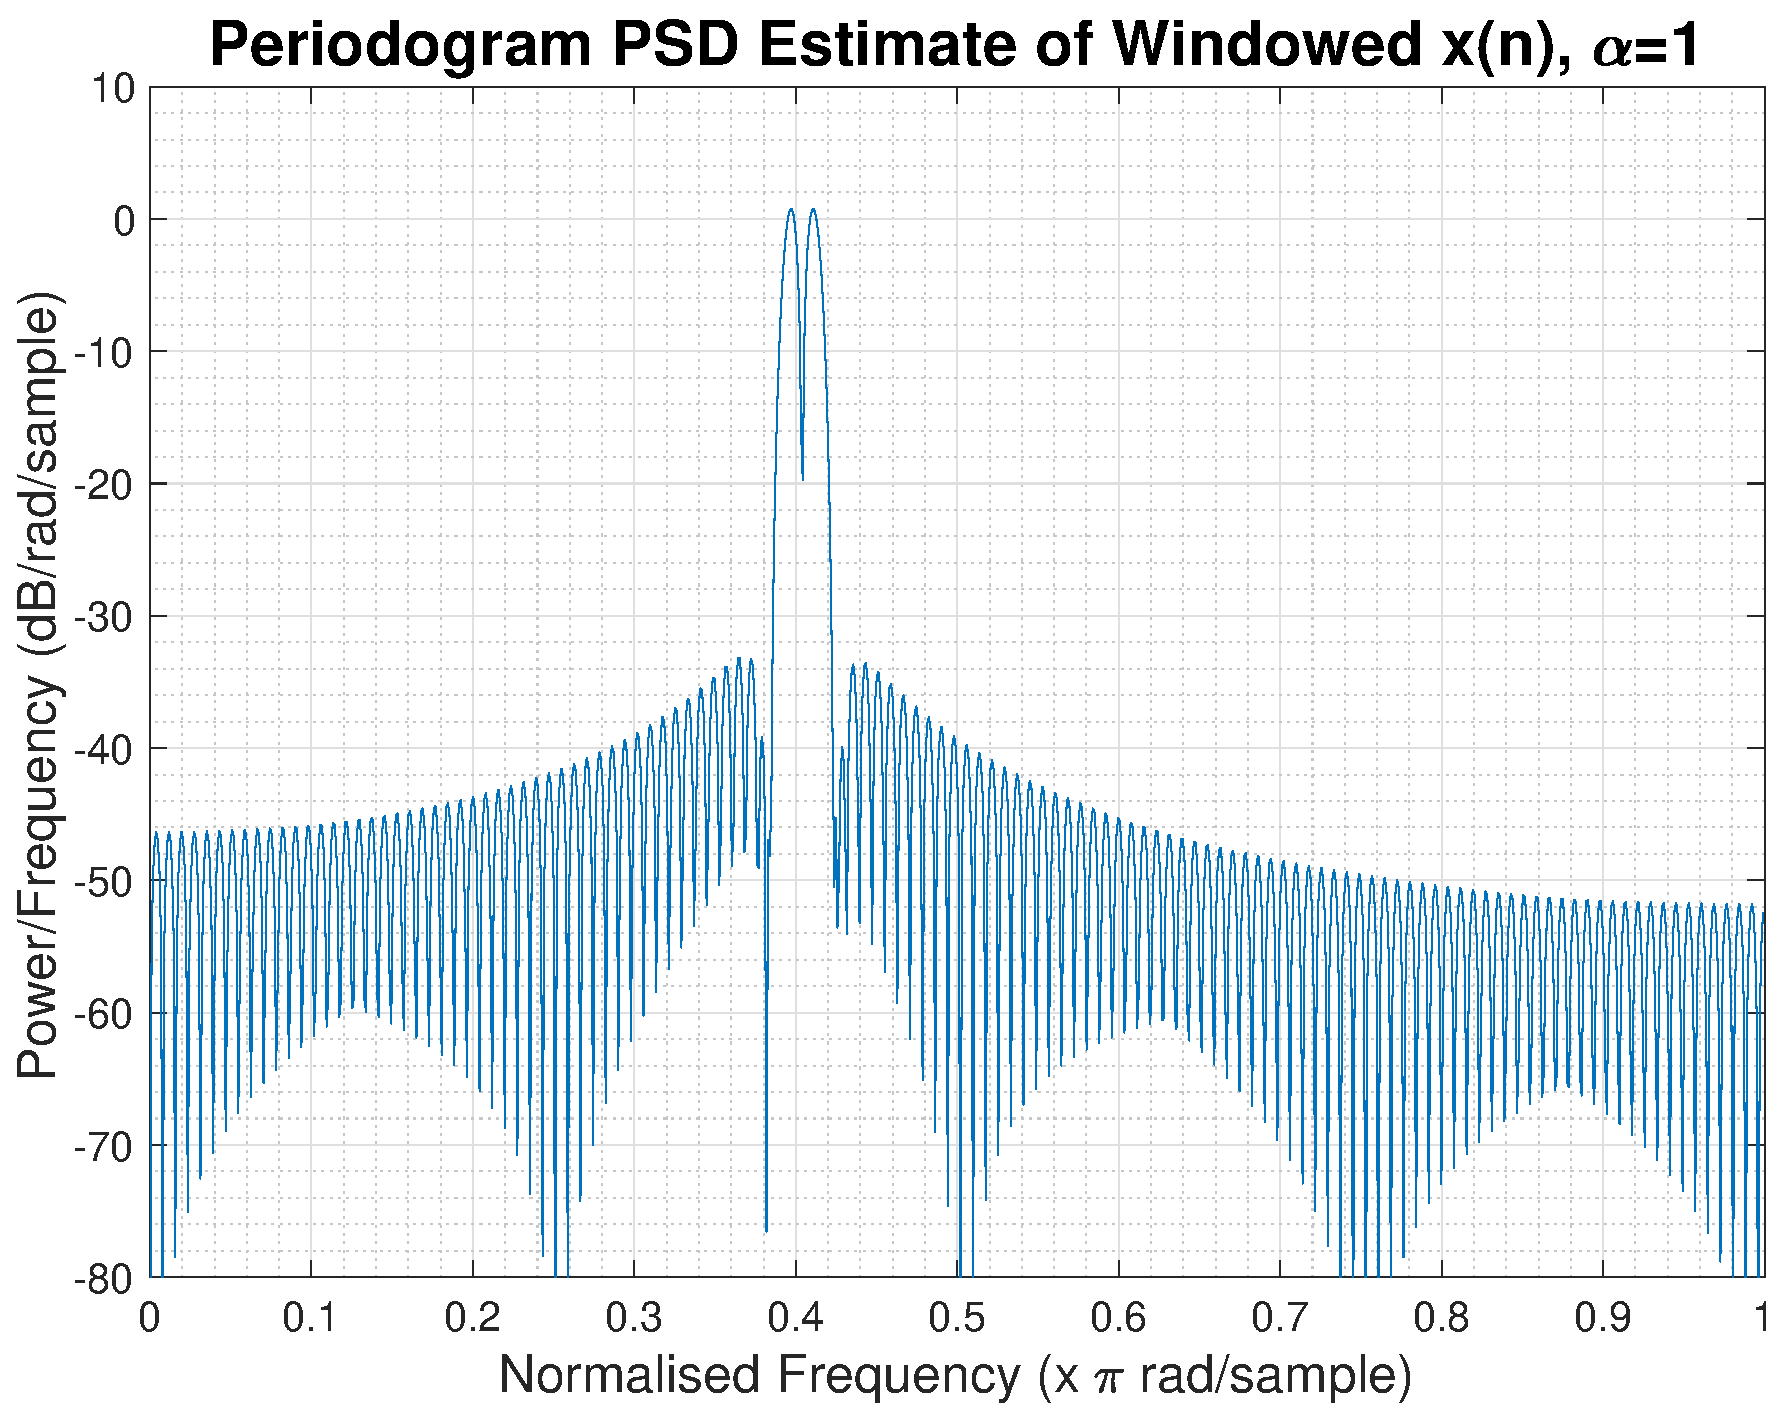
\includegraphics[width=0.32\textwidth]{part1/periodogram_windowed_xn_alpha_1}
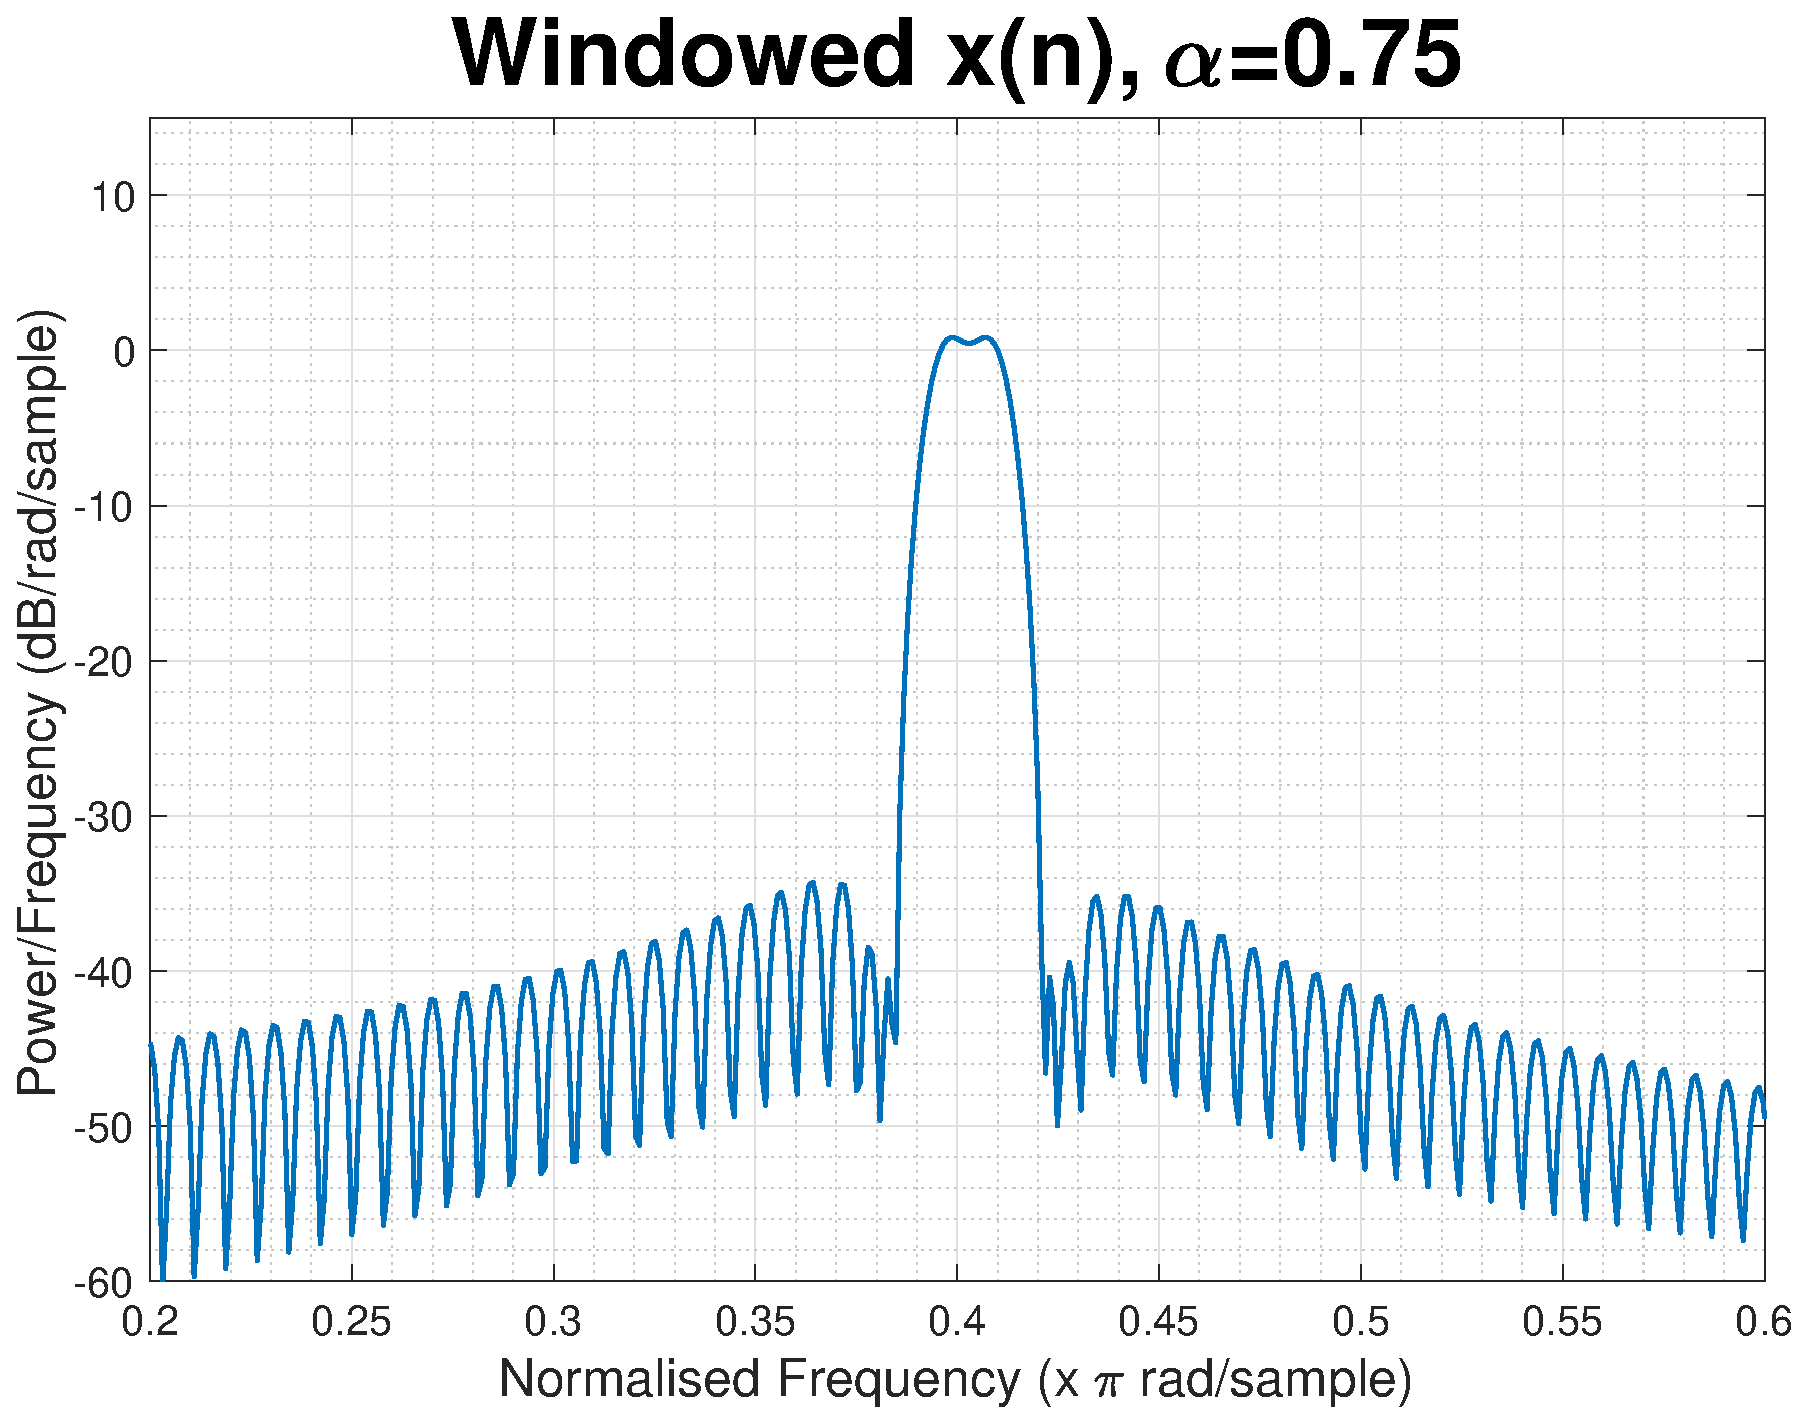
\includegraphics[width=0.32\textwidth]{part1/periodogram_windowed_xn_alpha_point_75}
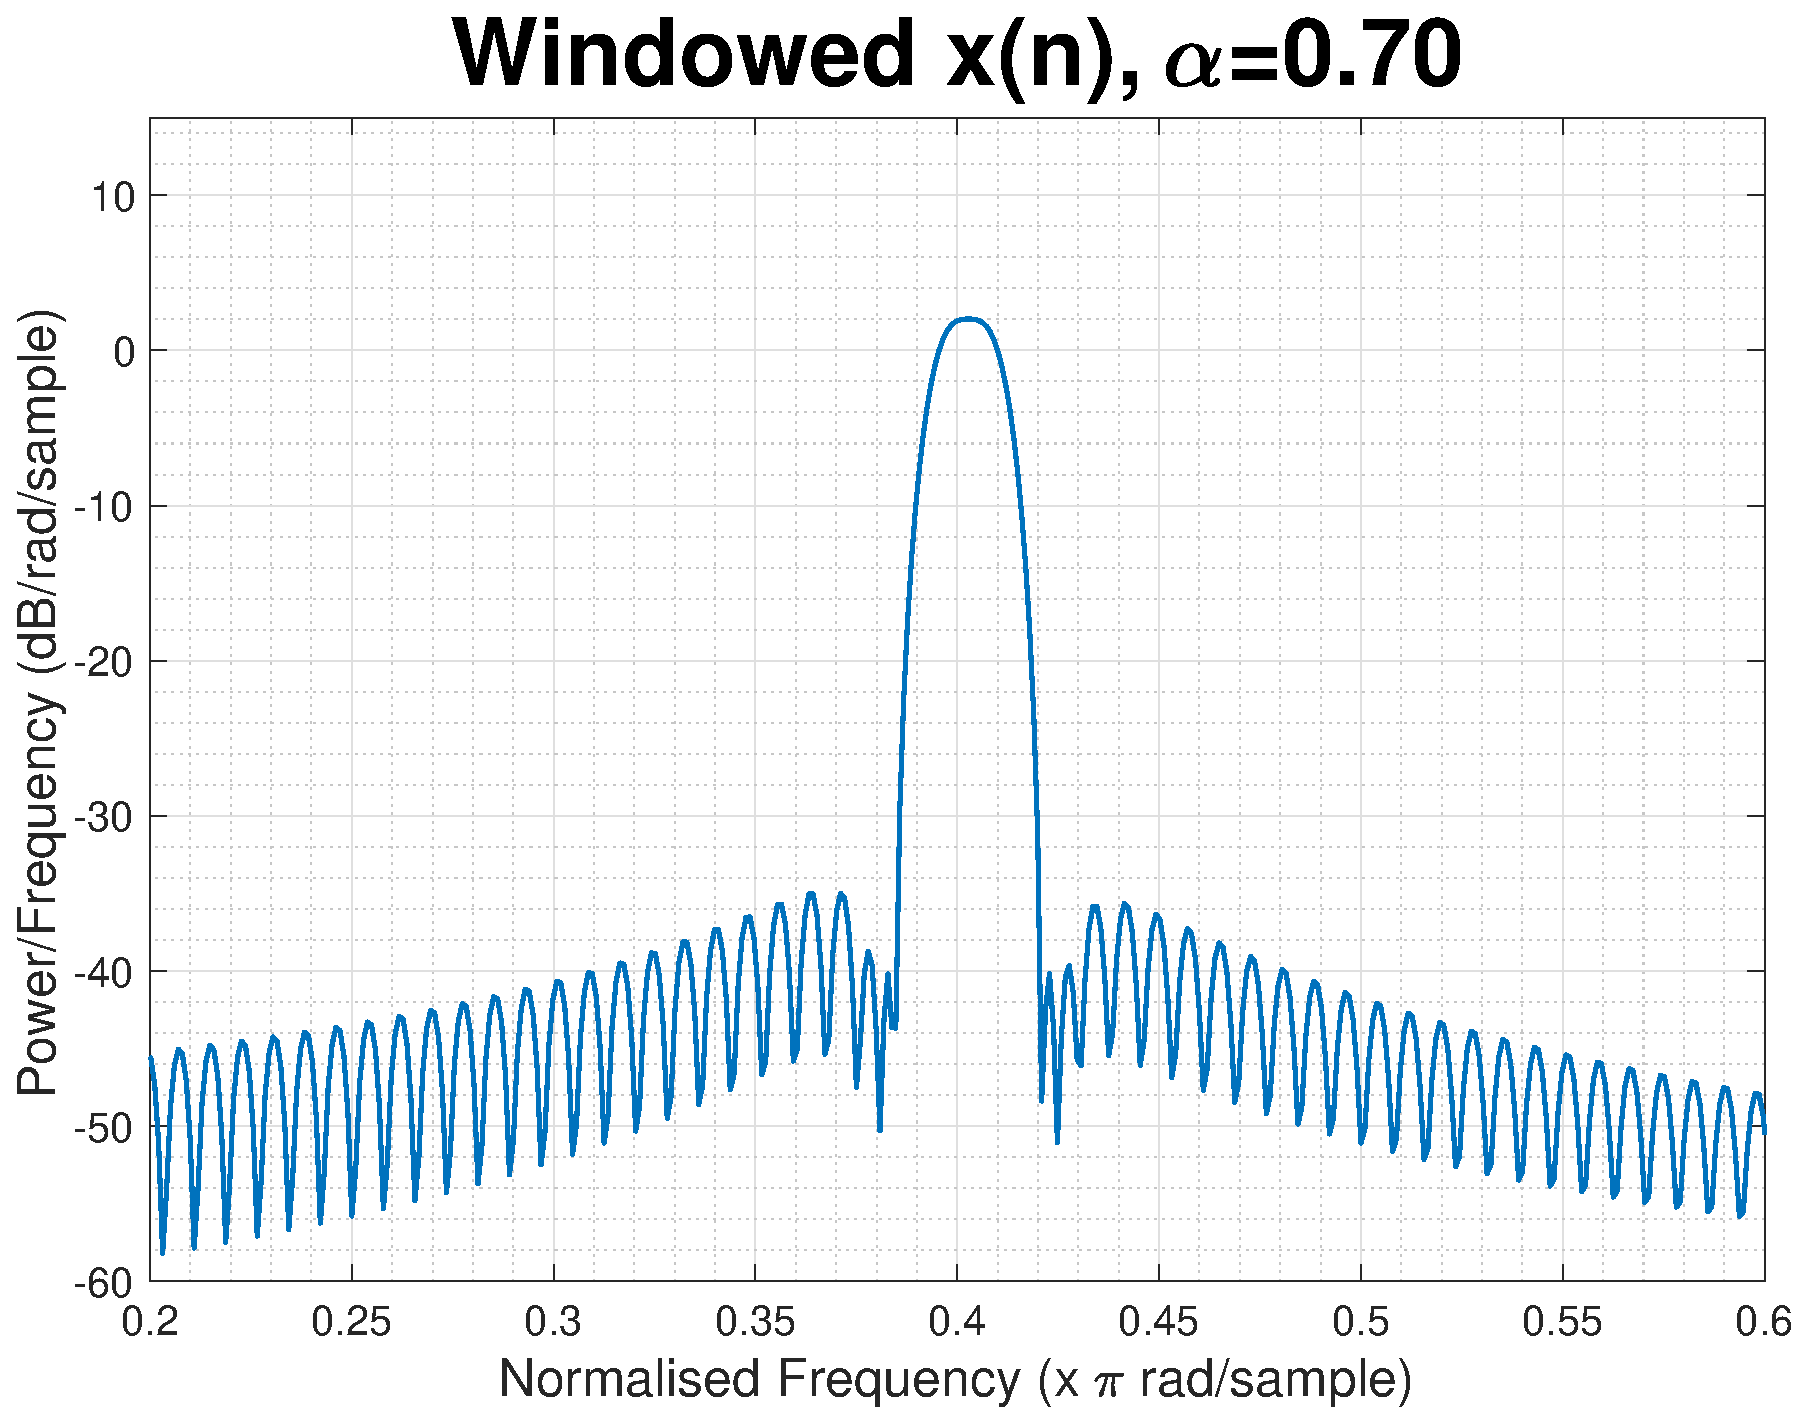
\includegraphics[width=0.32\textwidth]{part1/periodogram_windowed_xn_alpha_point_70}
\caption{Periodogram of Signal $x(n)$, Windowed using a Hamming Window, for Different Values of $\alpha$}
\end{figure}

\noindent{}d. Figure \ref{fig:bartlett_leakage} shows the periodograms obtained using the rectangular window. All windows have to trade-off the width of the mainlobe and the relative heights of the sidelobes. The rectangular window lies at an extreme end of this spectrum in that it has the smallest mainlobe however it also has the highest sidelobes. This causes the least amount of smearing and bias but results in the most spectral leakage. As such, the ability to distinguish the second peak deteriorates significantly as $a_2$ decreases. The amplitude threshold identification of the second sinusoidal term was slightly easier for $\alpha=12$ however it did not change significantly. The reason for this will be explained in the next part.

\begin{figure}[H]
\centering{}
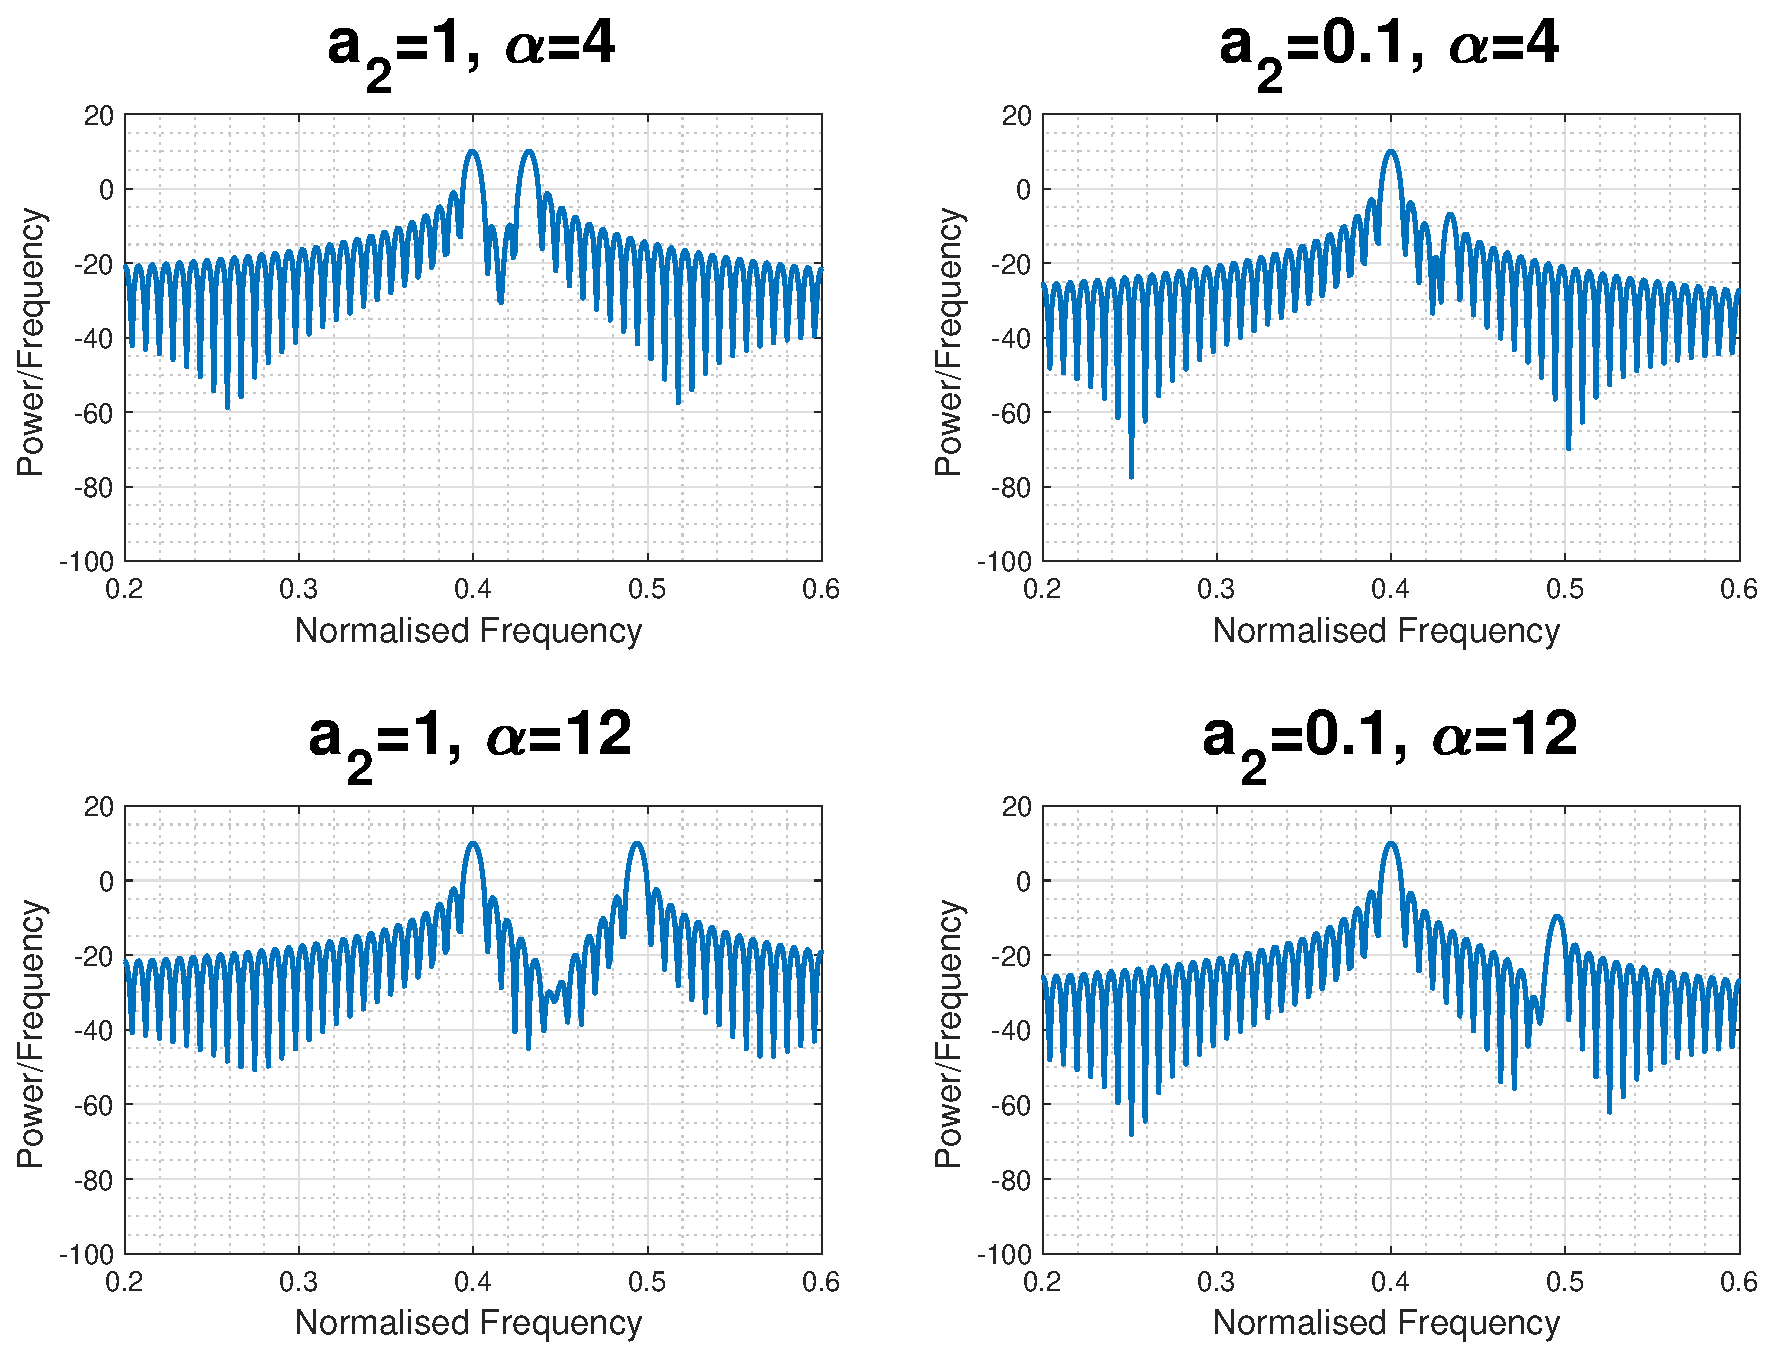
\includegraphics[width=0.48\textwidth]{part1/periodogram_leakage_bartlett_part_1}
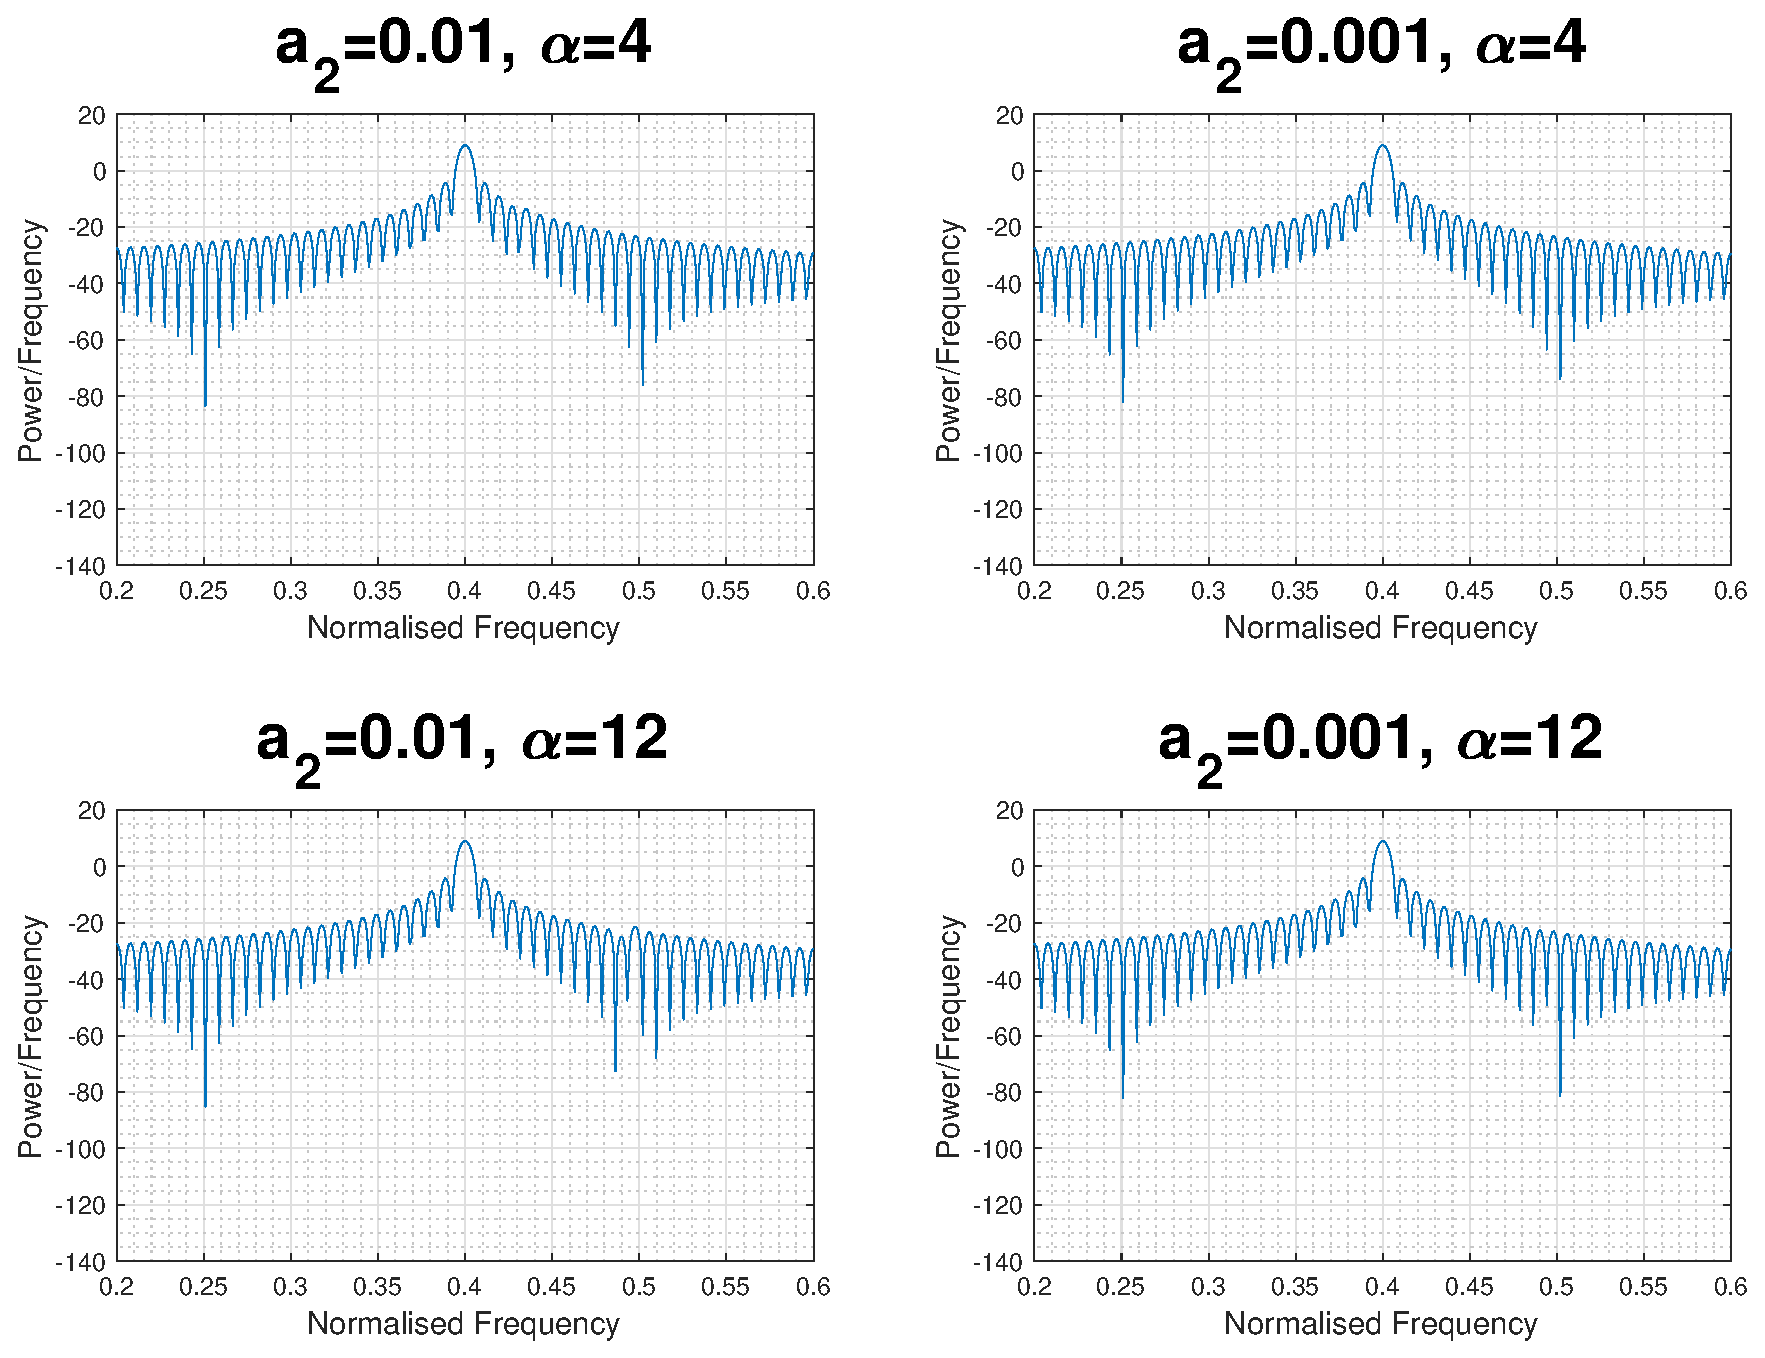
\includegraphics[width=0.48\textwidth]{part1/periodogram_leakage_bartlett_part_2}
\caption{Identification of Sinusoids using Rectangular Window}
\label{fig:bartlett_leakage}
\end{figure}

\noindent{}e. A rectangular window with $N=256$ can be thought of as a digital filter with $256$ zeros; as such, it is able to fix the gain to be 0 at 256 points. At frequencies, $f=4/N$ and $f=12/N$ the gain of the filter is 0. However, the sidelobes of the rectangular window are not constant and they decrease as distance from the mainlobe increases. As such, the amplitude threshold identification is slightly easier at $\alpha=12$ because the peak of sidelobes around $f=12/N$ is slightly lower than the peak of sidelobes around $f=4/N$.

\begin{figure}[H]
\centering{}
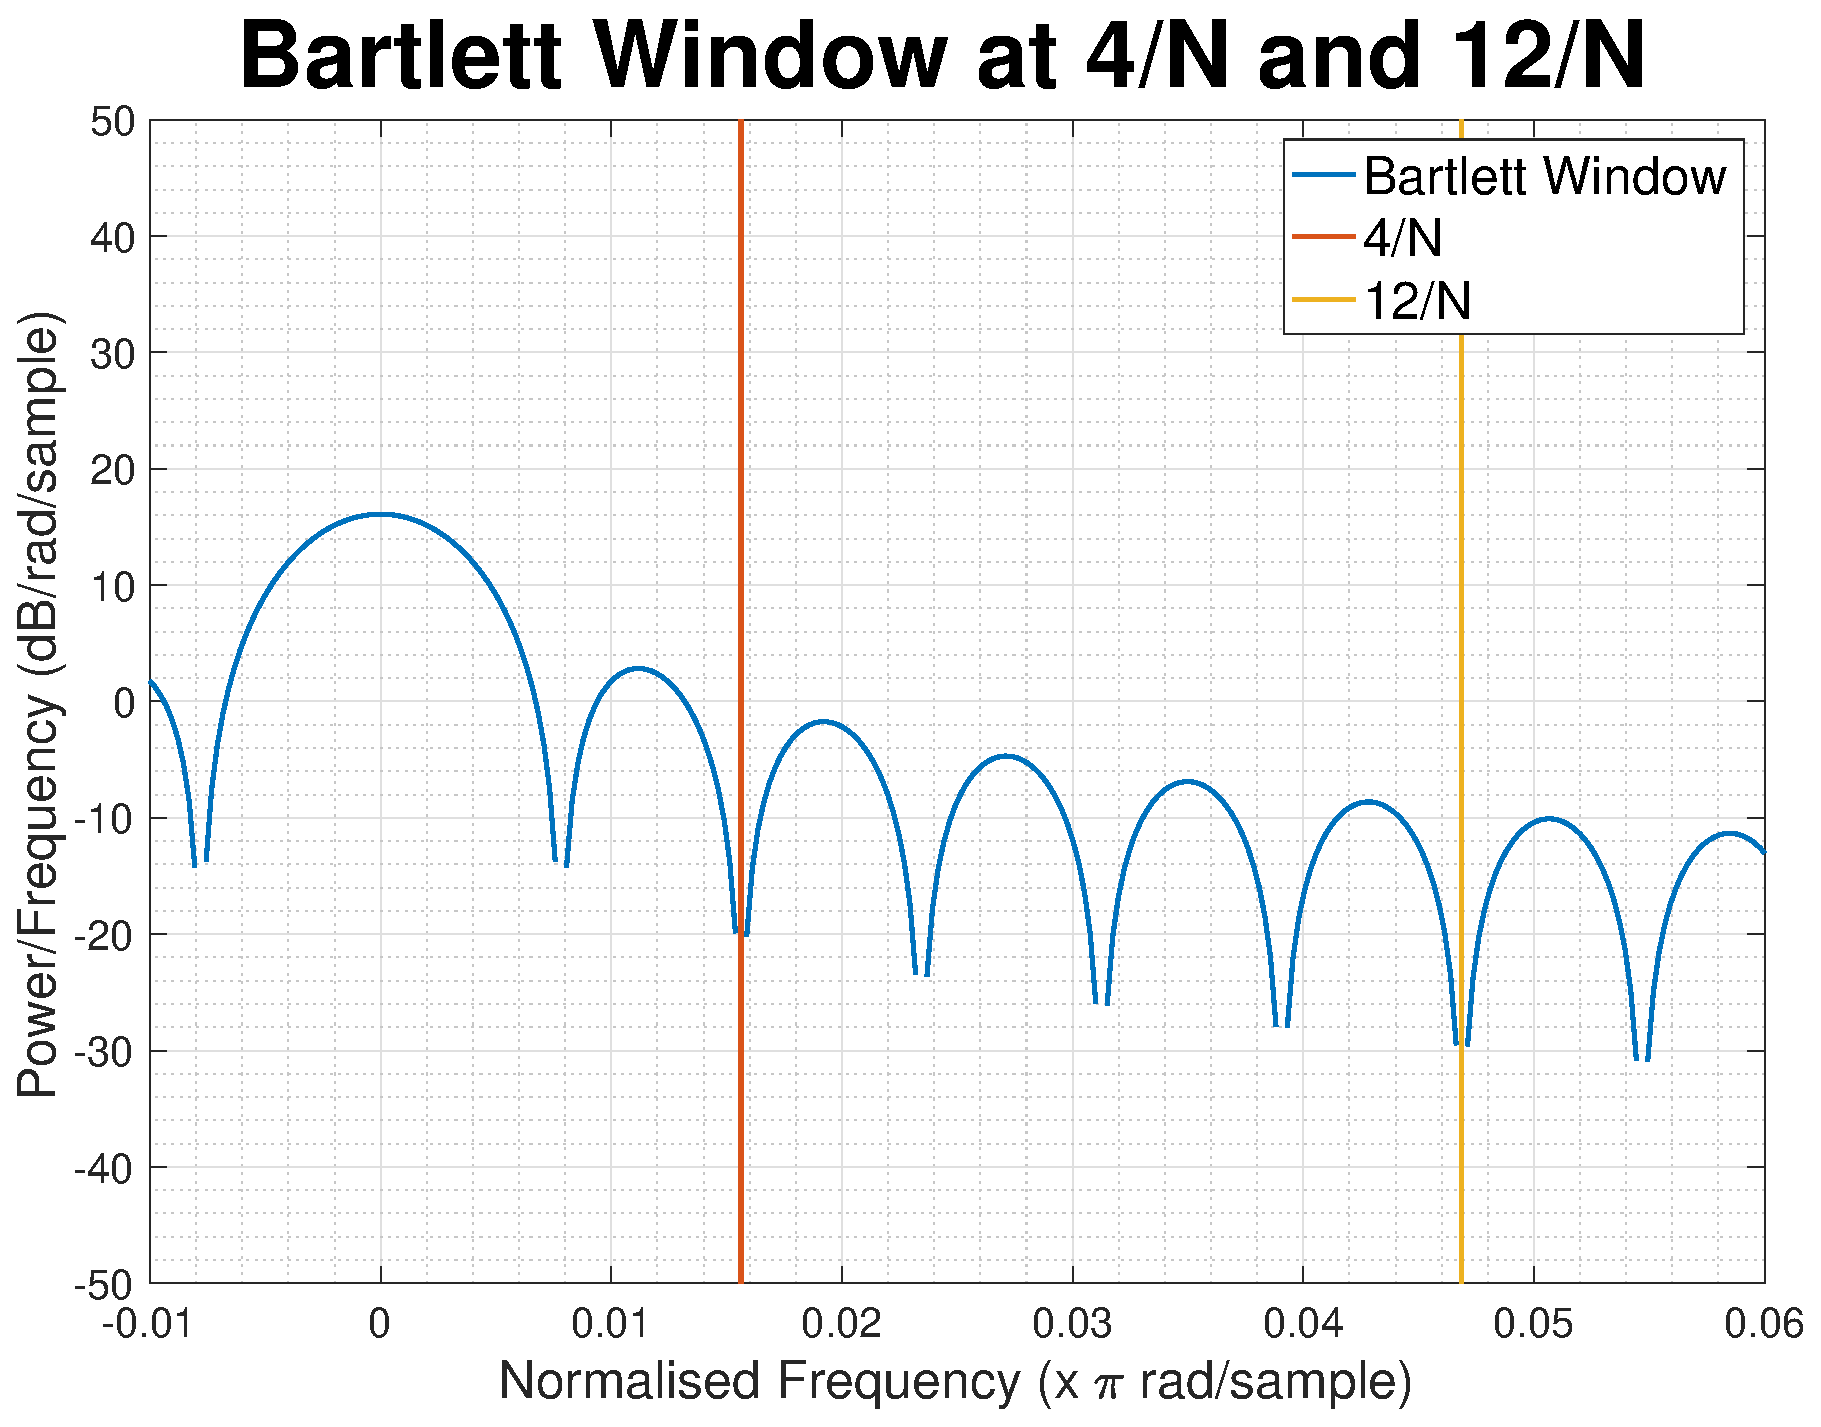
\includegraphics[width=0.32\textwidth]{part1/bartlett_amplitude}
\caption{Power Spectral Density of the Bartlett Window at $f=\frac{4}{N}$ and $f=\frac{12}{N}$}
\end{figure}

\noindent{}f. As shown in the figure below, it is possible to resolve the two components even when $a_2=0.001$. Notice that when the Chebyshev window is used, the overlapping of the mainlobes causes trouble when trying to distinguish between two frequencies; this is clear when $\alpha=4$. This was not the case when the rectangular window was used. Using the rectangular window, the height of sidelobes caused trouble when trying to distinguish between two frequencies. This represents the tradeoff that windows have to make between the width of the mainlobe as the height of the sidelobes. The rectangular window has a small mainlobe and thus the trouble in identification comes about because of the leakage effects whereas the Chebyshev window cause more smearing and less leakage.

\begin{figure}[H]
\centering{}
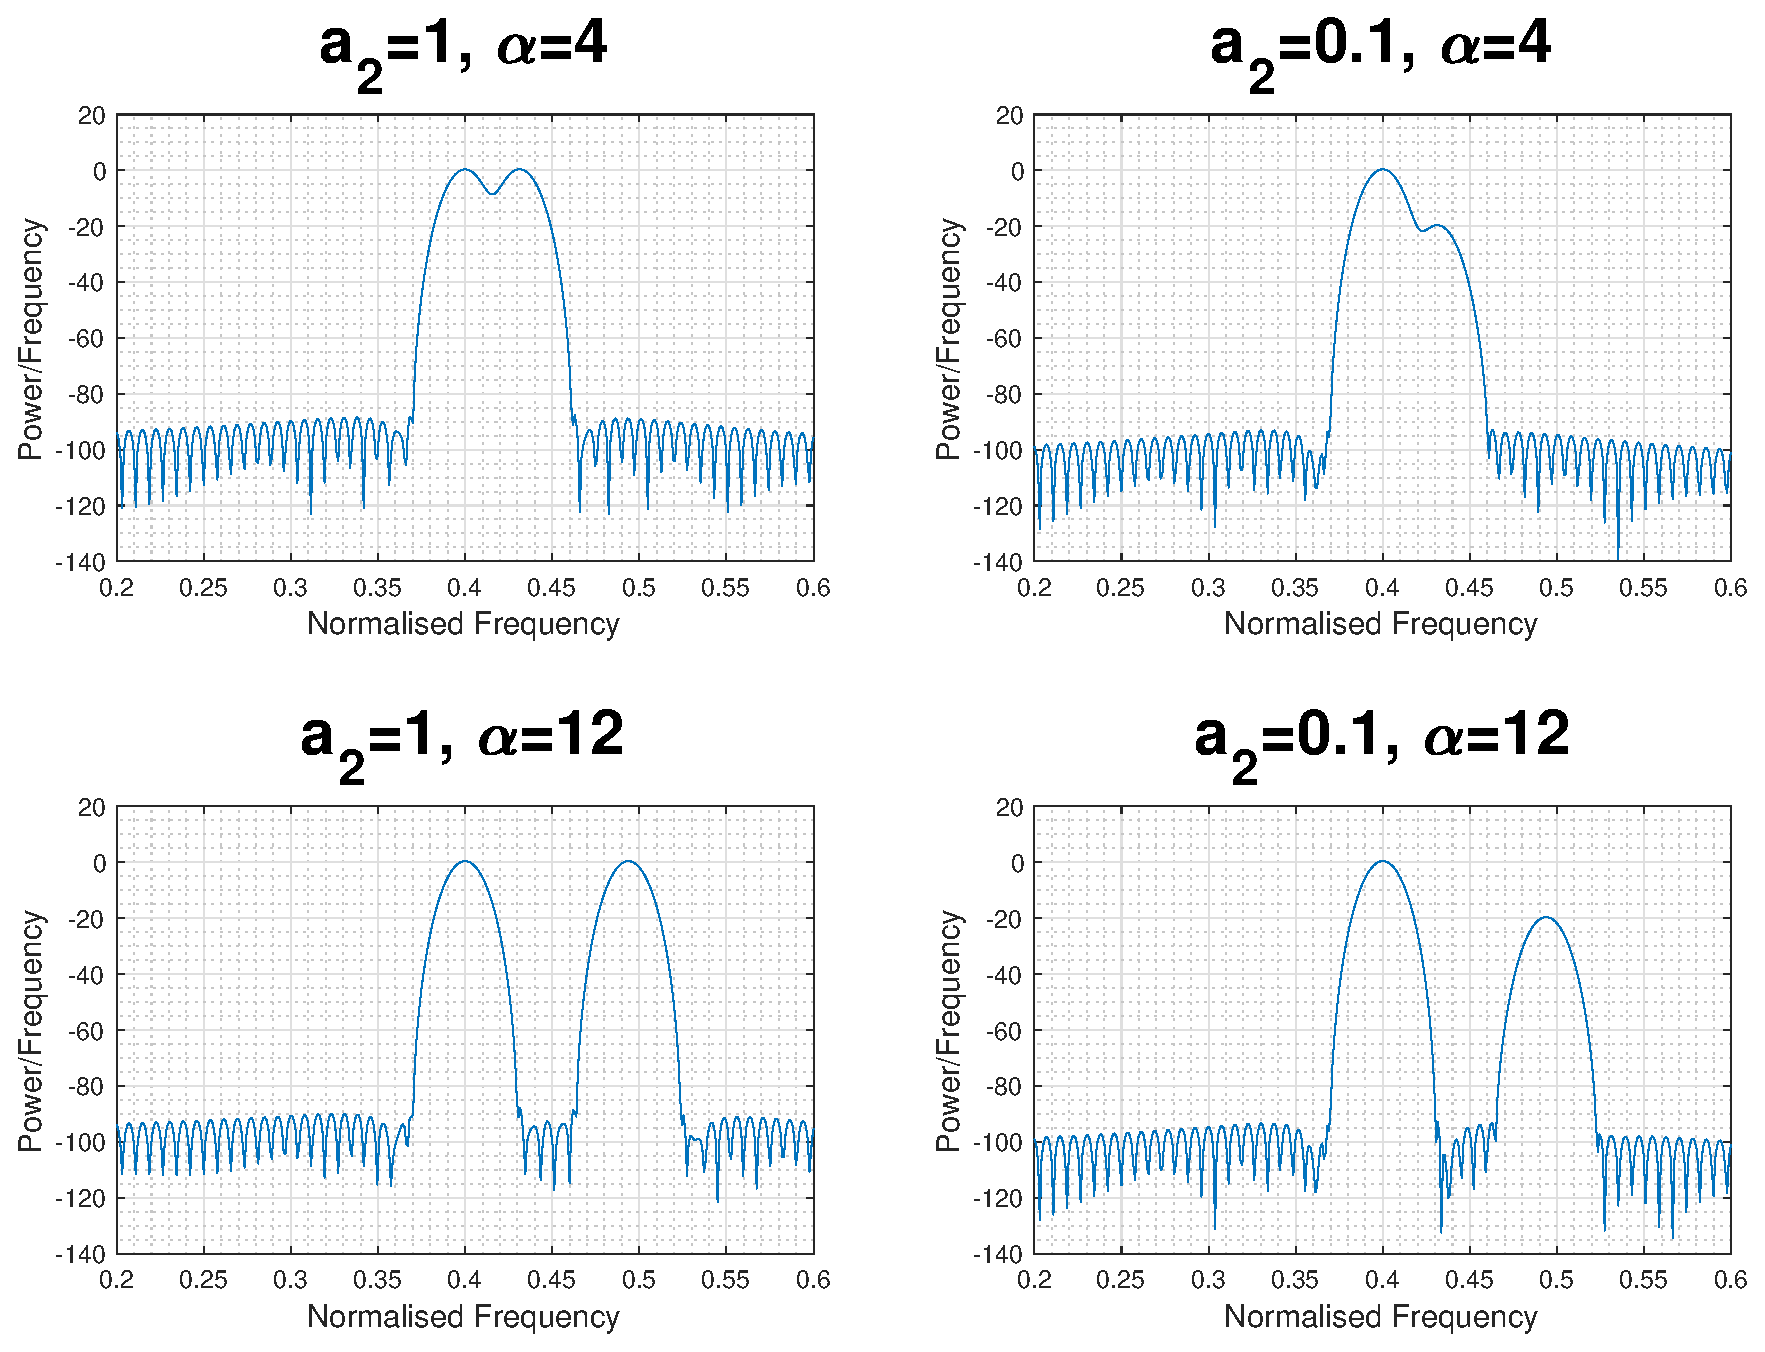
\includegraphics[width=0.48\textwidth]{part1/periodogram_leakage_chebwin_part_1}
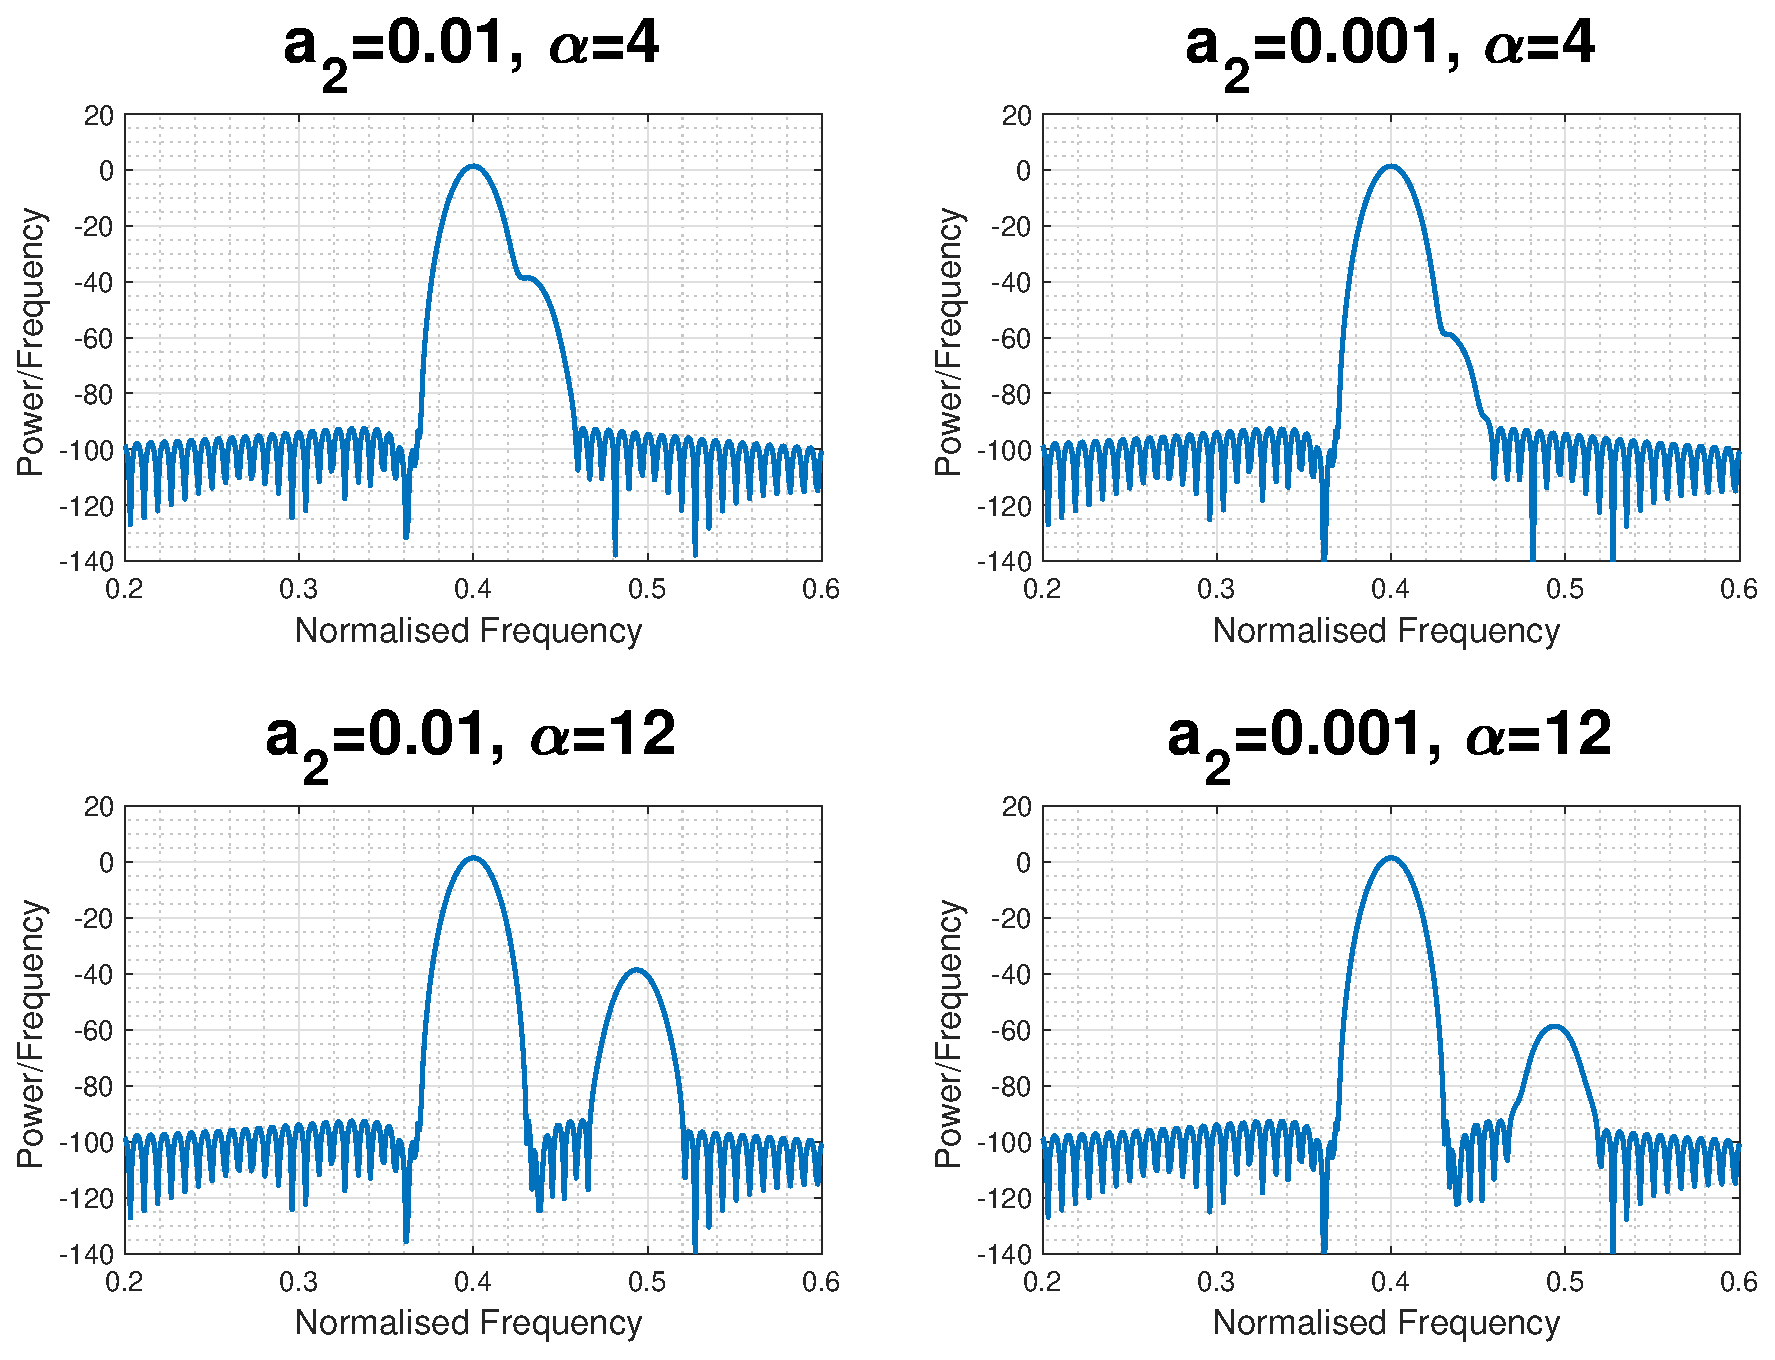
\includegraphics[width=0.48\textwidth]{part1/periodogram_leakage_chebwin_part_2}
\caption{Identification of Sinusoids using Chebyshev Window}
\end{figure}

\noindent{}The Blackman-Tukey method was used to find the periodograms and the results are shown below. The autocovariance function is calculated but only $64$ values are used; the tail end of the autocovariance is not reliable as they were calculated by averaging very few points and thus they are excluded when the Power Spectral Density is calculated. The results are not promising and the Blackman-Tukey method performs poorly compared to the Chebyshev window. However, this is completely expected. The Blackman-Tukey method is used to reduce the variance of the periodogram estimate by reducing the variance in the autocovariance estimate. A reduction is variance is traded-off for resolution; notice the number of troughs between the two peaks has reduced by a factor of $4$ when the Blackman-Tukey estimates are compared to the periodograms in Figure \ref{fig:bartlett_leakage}. This is expected since we have used $\frac{1}{4}$ the number of points to calculate the DFT. In this illustrative example, we have removed noise and thus the periodograms are determinstic and using the Blackman-Tukey method does not actually remove any noise variance, it just reduces the resolution and thus depreciates our ability to distinguish between two frequencies.

\begin{figure}[H]
\centering{}
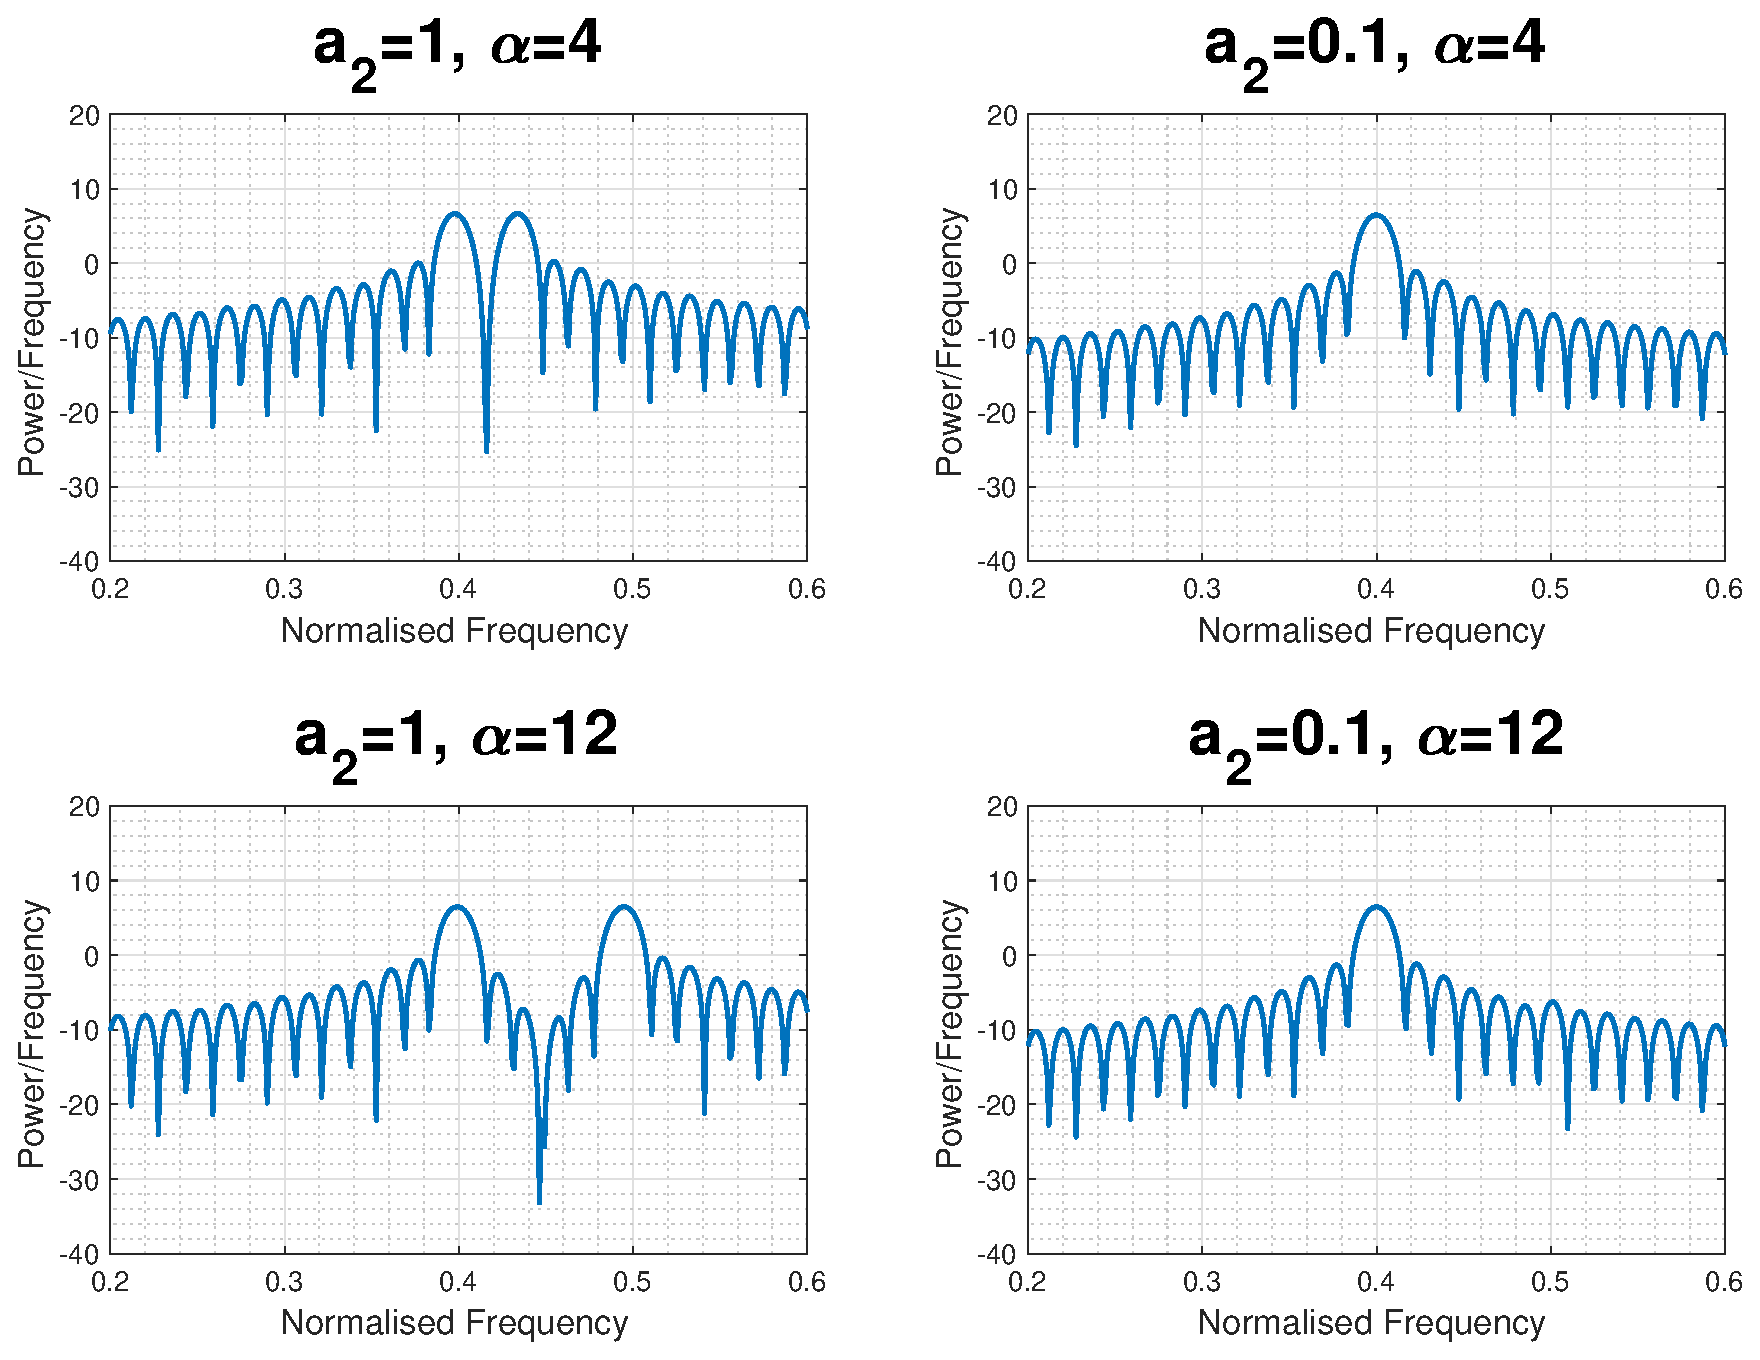
\includegraphics[width=0.48\textwidth]{part1/periodogram_leakage_blackman_tukey_part_1}
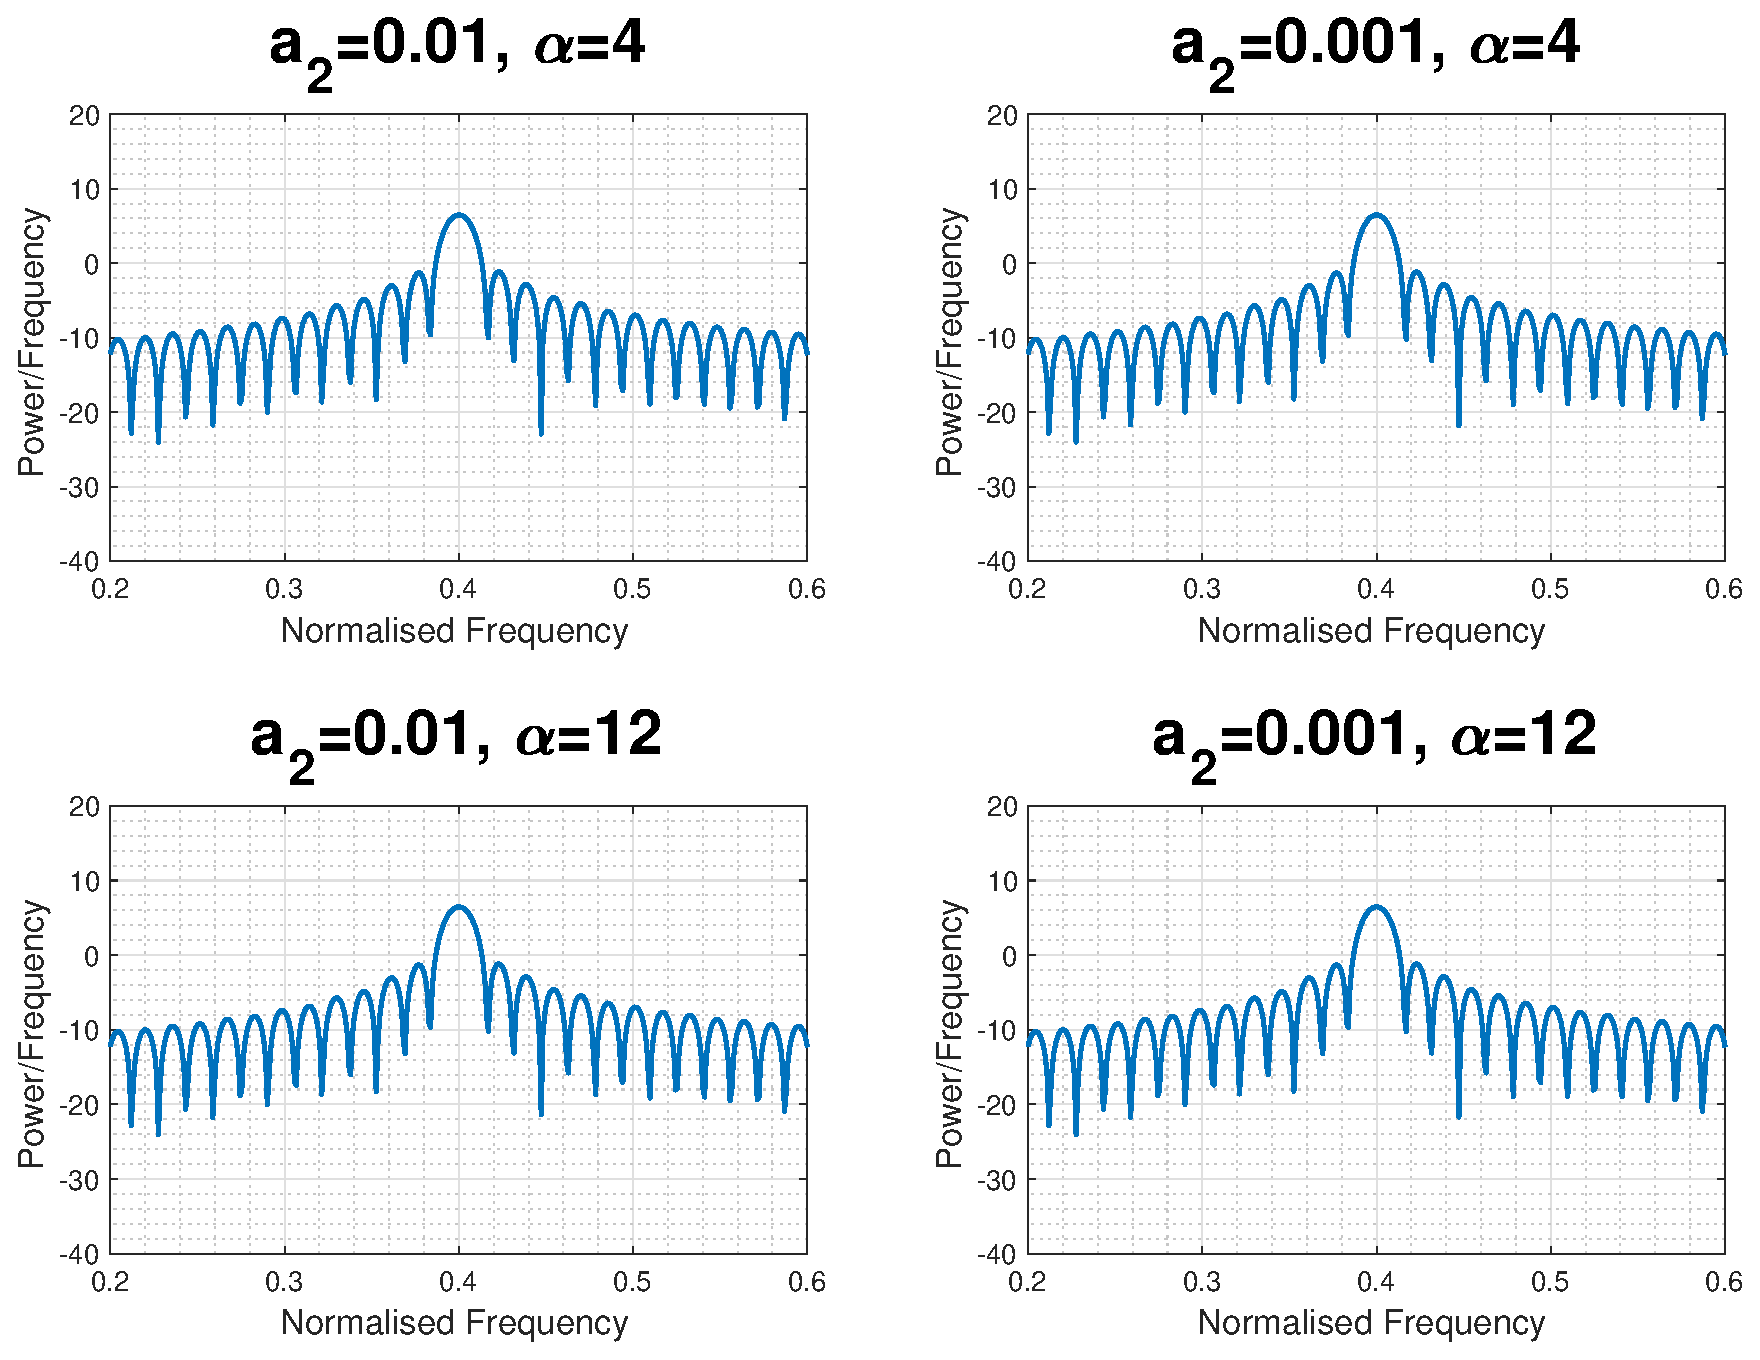
\includegraphics[width=0.48\textwidth]{part1/periodogram_leakage_blackman_tukey_part_2}
\caption{Blackman-Tukey Method for Identification of Two Sinusoidal Tones}
\end{figure}

\newpage
\subsection{Periodogram-based Methods Applied to Real-World Data}

\noindent{}a. The figure below shows the periodogram, with and without pre-processing, for the sunspot time series. It is evident that the periodograms produced by removing the mean and removing the trend are very similar. These two periodograms are also extremely similar to the original periodogram beyond $f_n=0.2$.

\begin{figure}[H]
\centering{}
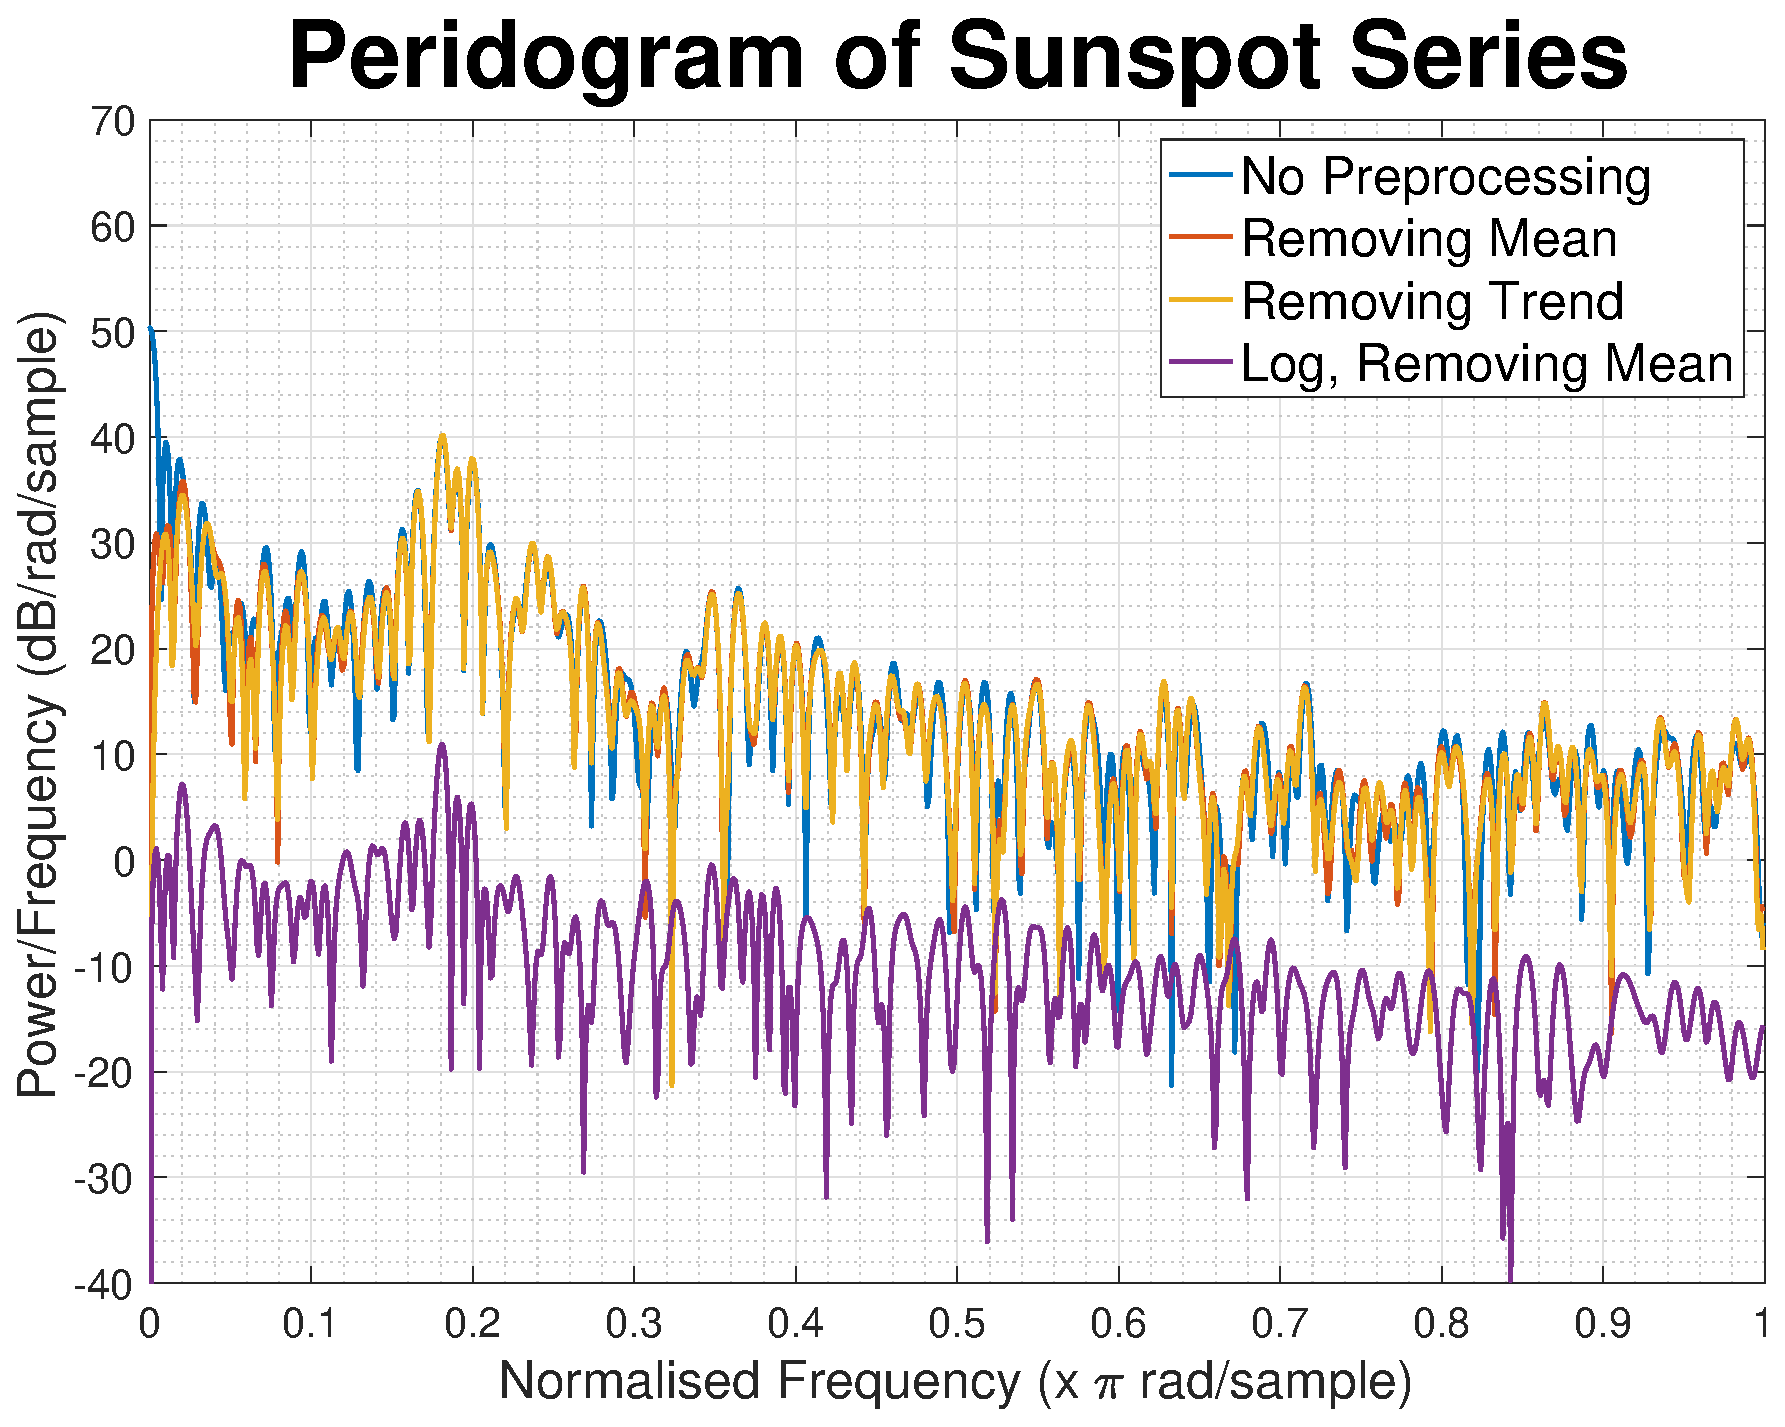
\includegraphics[width=0.33\textwidth]{part1/sunspot_periodogram}
\caption{Standard Periodogram, with and without Preprocessing, for Sunspot Time Series}
\end{figure}

\noindent{}The original periodogram has a DC component that causes the periodogram to have a spike at $f=0$ of approximately 50 dB. The removal of the mean removes the the spectral components close to $f=0$. The mean can be visualized as a rectangular signal that has been added to a zero-mean signal. Through the linearity of the Fourier Transform and the fact that the spectrum of a rectangular signal is a \textit{sinc}, the spectrum of the mean-removed signal only differs from the original signal at low frequencies. The \texttt{detrend} function removes linear trends. The Fourier Transform of linear functions is a spike at $f=0$ and a magnitude proportional to $\frac{1}{f^2}$ for $f \neq 0$. As such, using \texttt{detrend} prior to formulating the periodogram also only alters low frequency components. \\

\noindent{}Note that before we are able to take logarithms of the time-series, a small offset of $0.001$ was added to the entire series. This allowed the logarithms to be taken because the sunspot series has values of $0$ at certain points. Since this offset is added to all the terms, it too was removed when the mean of the series was subtracted. The shape of the periodogram obtained is similar to the periodogram obtained solely by removing the mean and tread. The main difference is in the fact that spikes have been greatly accentuated. \\

\noindent{}b. The standard periodogram of the EEG obtained from an electrode located at the POz region of the head is graphed in the figure below. \textbf{The peaks in the spectrum corresponding to the SSVEP are clearly observed at $f=13,26,39,52$.} As expected, the fundamental frequency response peak is the largest whereas the height of the harmonics is monotonically decreasing.

\begin{figure}[H]
\centering{}
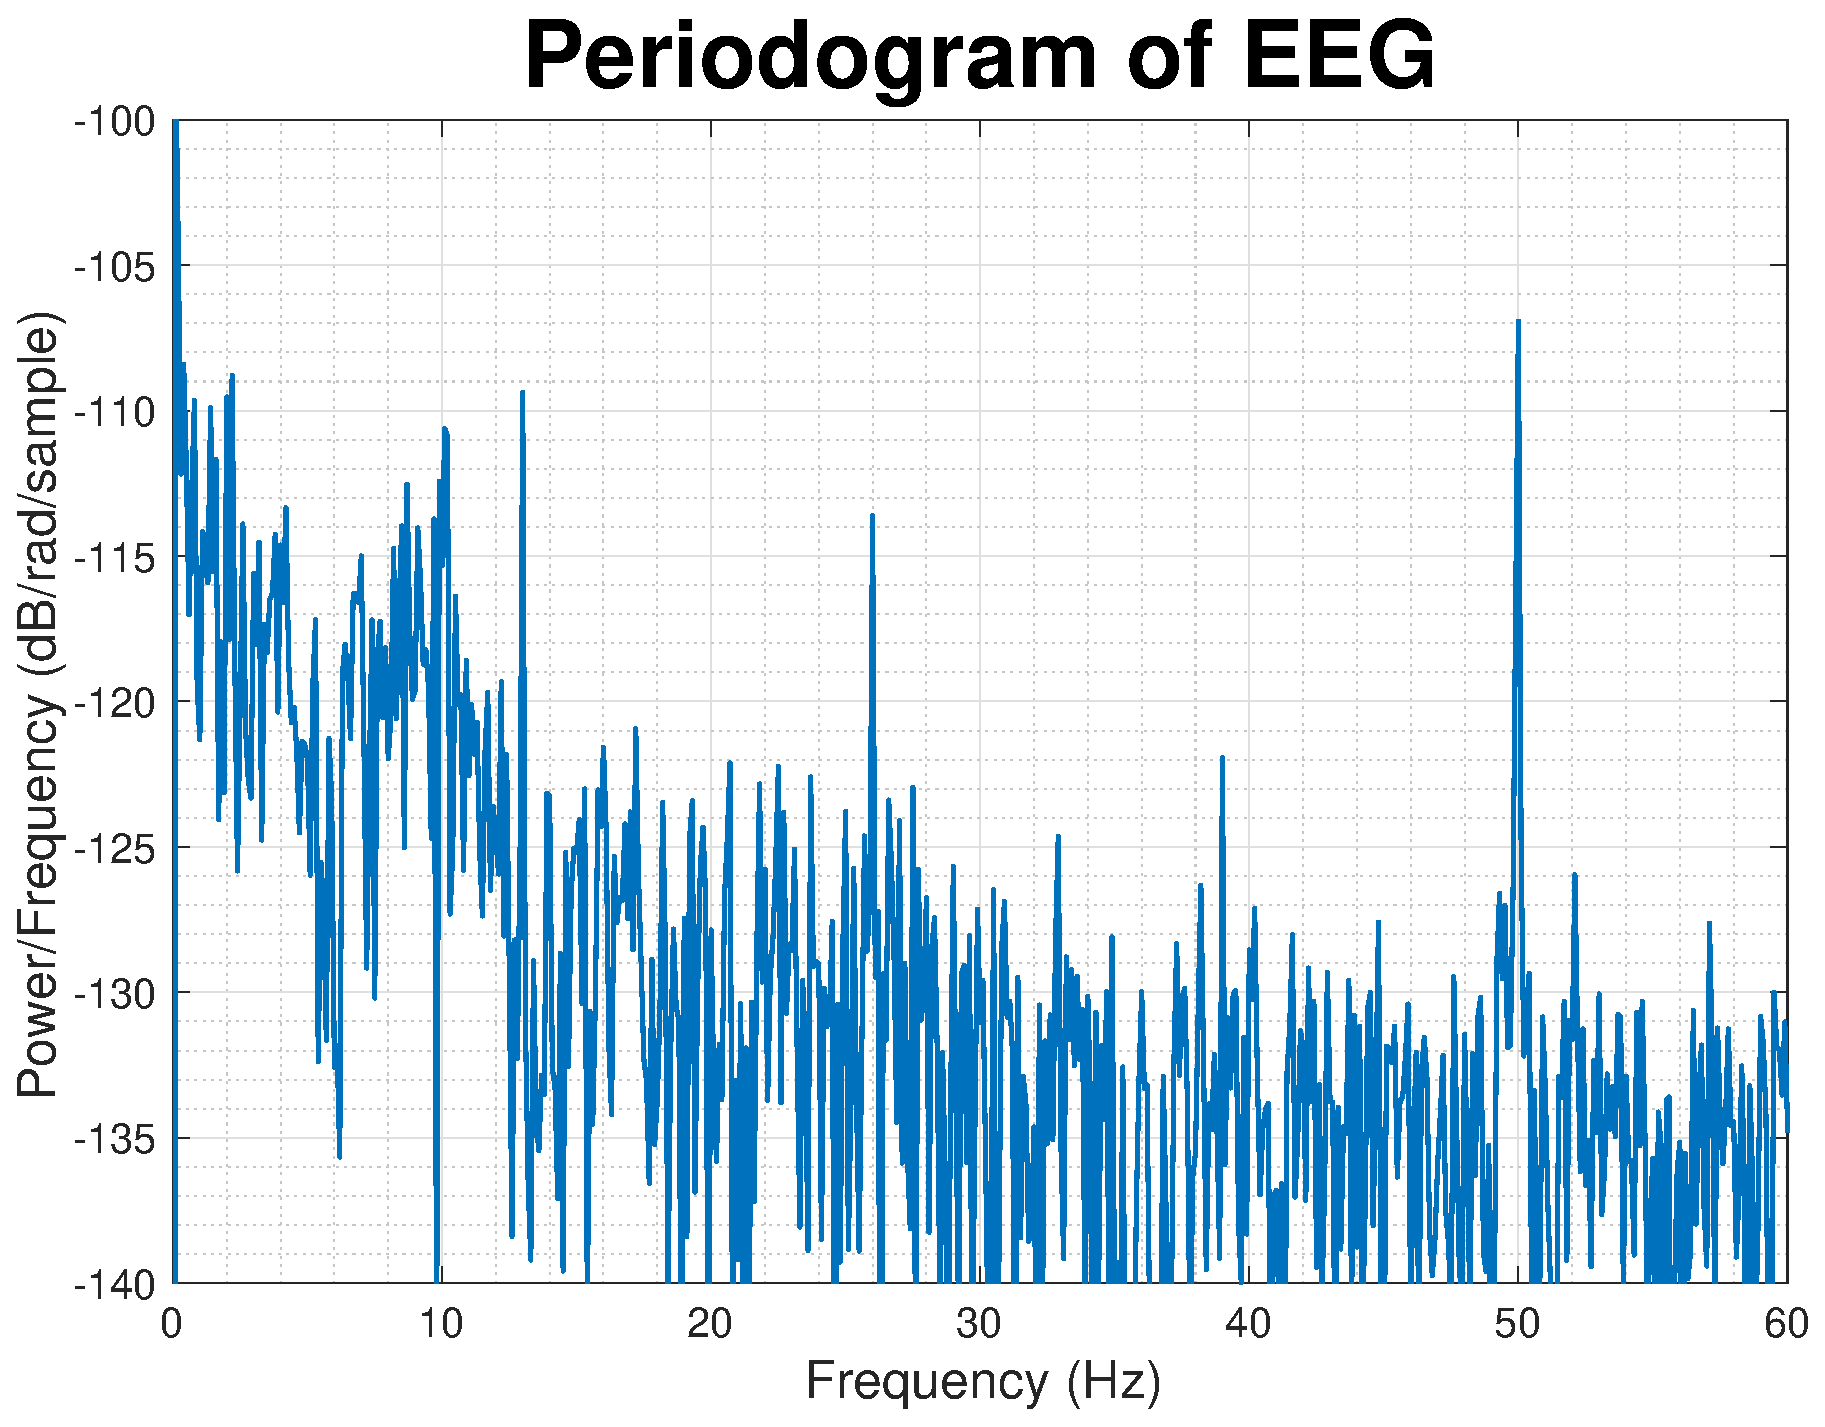
\includegraphics[width=0.33\textwidth]{part1/POz_standard_periodogram}
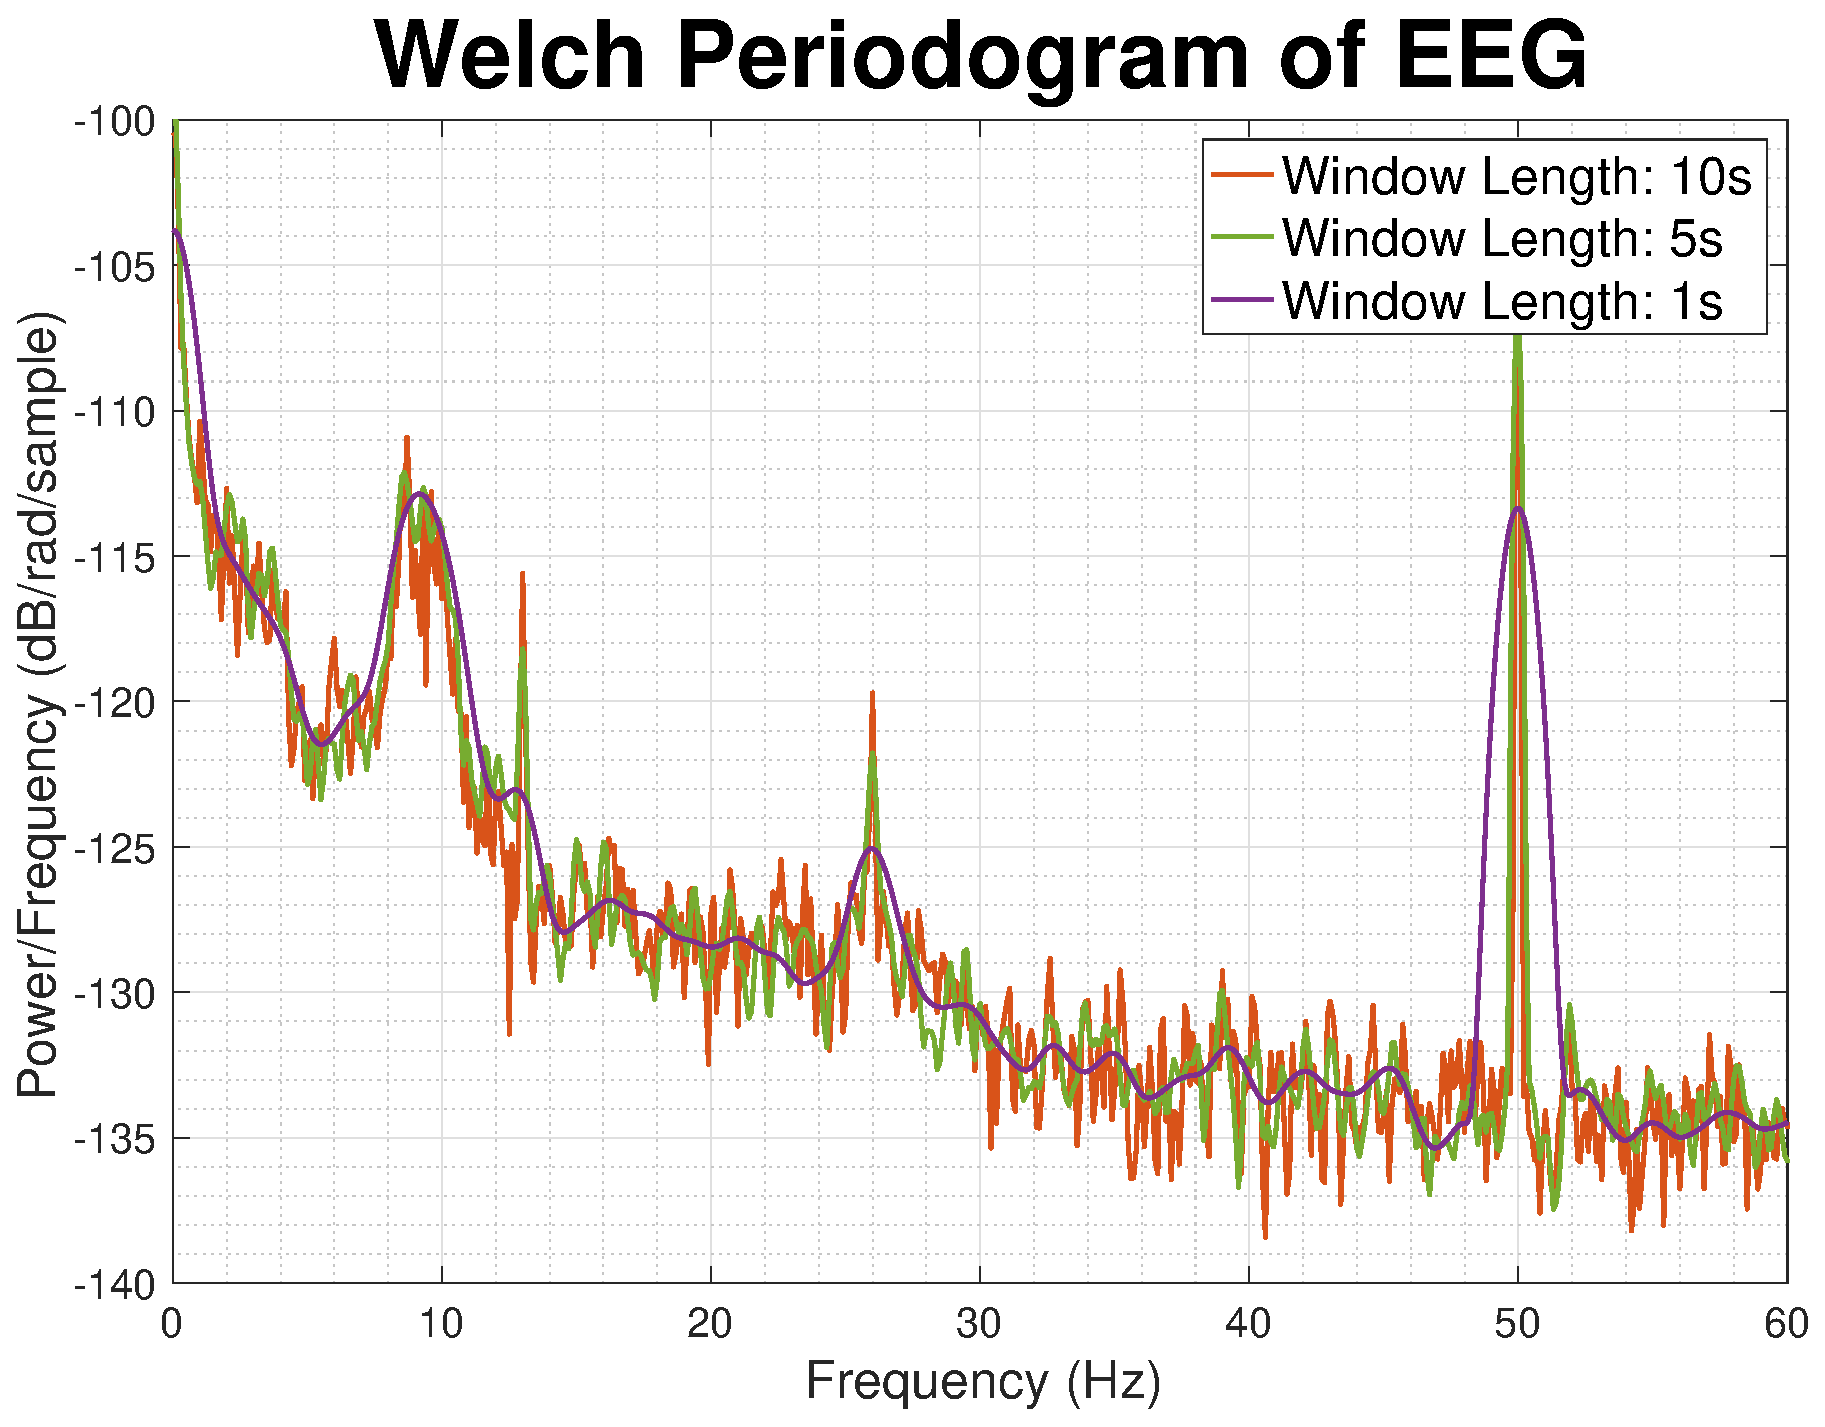
\includegraphics[width=0.33\textwidth]{part1/POz_welch_periodogram}
\caption{Standard Periodogram and Bartlett Periodogram with Hamming Window for EEG samples Obtained from POz Location on the Scalp}
\end{figure}

\noindent{}The figure also shows the Bartlett periodograms obtained by averaging the signal over different window lengths (10 s, 5 s, 1 s). As the duration of the observation window becomes smaller, the variance of the periodogram decreases. A smaller observation window means that the number of periodograms obtained increases; there are a greater number of periodograms to average over and thus the variance decreases. However, using a shorter observation window means that the frequency resolution of the periodogram has decreased. The damning effect of decreasing the frequency resolution is evident when the periodogram obtained from by averaging over 1 s windows is studied; the peridogram has been graphed again in Figure \ref{fig:bartlett_1_sec} to emphasize the difficulty in identifying SSVEP peaks. The large alpha-rhythm present in the EEG have masked the distinct peak that occurs at $13$ Hz. This makes identifying the fundamental frequency response peak much harder. Notice that the first harmonic at $f_n=26$ Hz is still visible. This is due to the fact that there are no large frequency components around $f=26$ Hz that can cause spectral leakage and thus mask the harmonic. Note that the extremely large frequency component at 50 Hz has completely masked the 3rd harmonic that is visible in the original, unaveraged periodogram. The component at 50 Hz is so strong that the shape of the power spectrum of rectangular window used is evident in Figure \ref{fig:bartlett_1_sec}.

\begin{figure}[H]
\centering{}
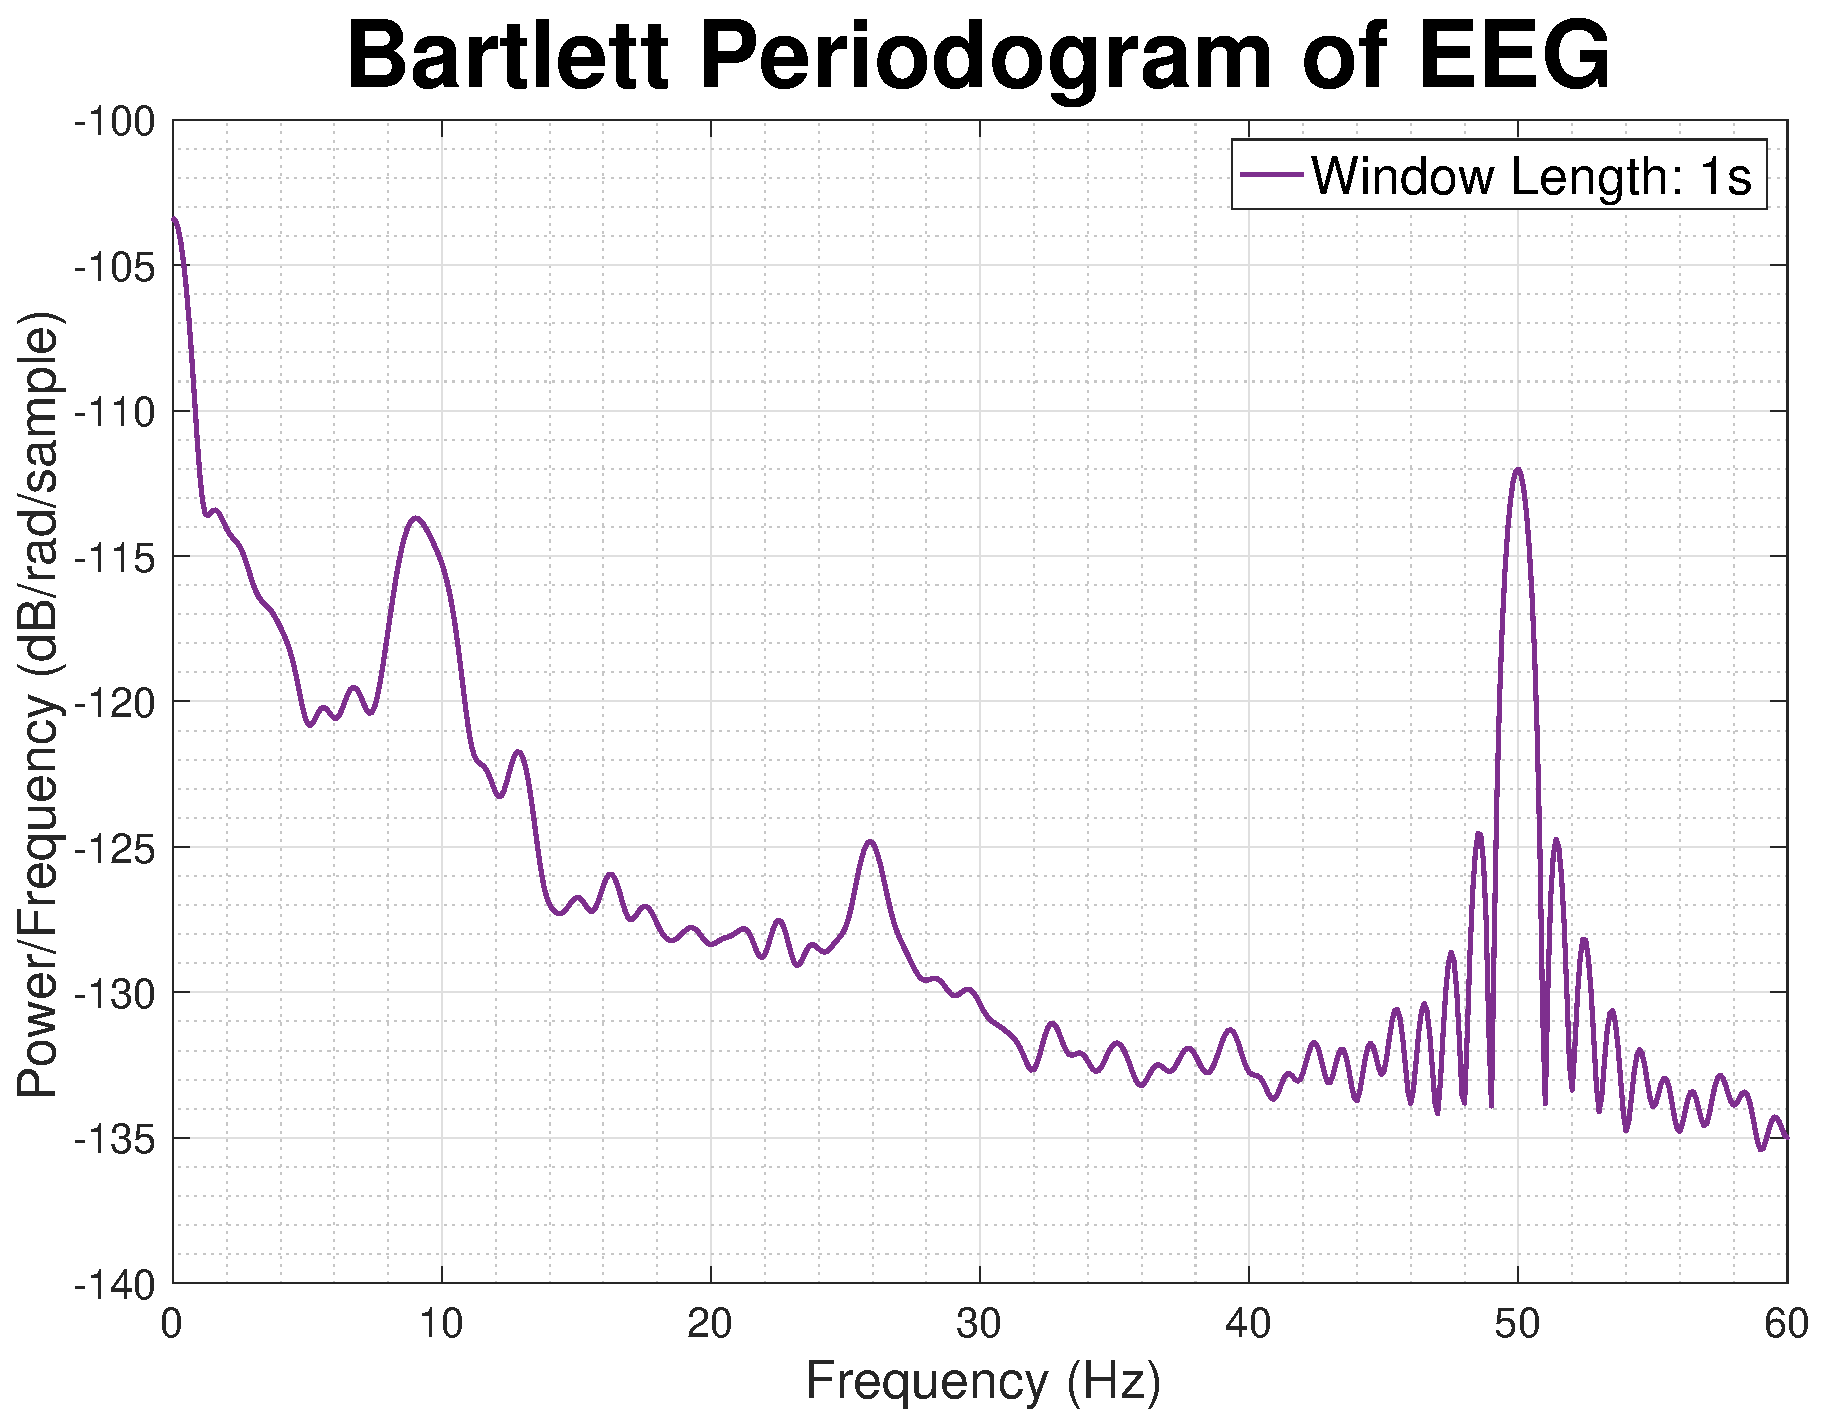
\includegraphics[width=0.33\textwidth]{part1/POz_welch_periodogram_1_sec}
\caption{Bartlett Periodogram with Hamming Window averaged over 1 s intervals}
\label{fig:bartlett_1_sec}
\end{figure}

\noindent{}This shows the clear trade off between frequency resolution and variance reduction that has to be made when averaging periodograms. 
